\documentclass{article} % For LaTeX2e
\PassOptionsToPackage{numbers,compress}{natbib}
% \PassOptionsToPackage{numbers}{natbib}
\usepackage[preprint]{style/arxiv}

\usepackage{amsmath,amssymb,amsthm,amsfonts,bm}
\usepackage{booktabs}
\usepackage{array}
\usepackage{colortbl}
\usepackage{mathtools}
\usepackage{thmtools}
\usepackage{booktabs}
\usepackage{xfrac}
\usepackage{xspace}
\usepackage{graphicx}
% \usepackage[dvipsnames]{xcolor}
% \usepackage[colorlinks=true,linkcolor=blue,citecolor=blue,urlcolor=blue]{hyperref}
\usepackage[normalem]{ulem}
% \usepackage{subcaption}
\usepackage{subfigure}
\usepackage{todonotes}
\usepackage[toc,page,header]{appendix}
\usepackage{minitoc}
\usepackage{url}
\usepackage{comment}
\usepackage{algorithm} % algorithmic
\usepackage{wrapfig}
\usepackage{multirow}
\usepackage{multicol}
\usepackage[T1]{fontenc}
\usepackage{hyperref}
\usepackage{url}
\usepackage{cleveref}
\usepackage{enumitem}
\usepackage{soul}
\setuldepth{Test}
\usepackage[noend]{algpseudocode}
\creflabelformat{equation}{#2\textup{#1}#3}

\renewcommand \thepart{}
\renewcommand \partname{}

% theorem stuff
\newtheorem{lemma}{Lemma}
\newtheorem{remark}{Remark}
\newtheorem{proposition}{Proposition}
\newtheorem{definition}{Definition}
\newtheorem{theorem}{Proposition}
\newtheorem{corollary}{Corollary}
\newtheorem{assumption}{Assumption}
\usepackage{caption}
\captionsetup{font=small}

%%%%% NEW MATH DEFINITIONS %%%%%

\usepackage{amsmath,amsfonts,bm}

% Mark sections of captions for referring to divisions of figures
\newcommand{\figleft}{{\em (Left)}}
\newcommand{\figcenter}{{\em (Center)}}
\newcommand{\figright}{{\em (Right)}}
\newcommand{\figtop}{{\em (Top)}}
\newcommand{\figbottom}{{\em (Bottom)}}
\newcommand{\captiona}{{\em (a)}}
\newcommand{\captionb}{{\em (b)}}
\newcommand{\captionc}{{\em (c)}}
\newcommand{\captiond}{{\em (d)}}

% Highlight a newly defined term
\newcommand{\newterm}[1]{{\bf #1}}


% Figure reference, lower-case.
\def\figref#1{figure~\ref{#1}}
% Figure reference, capital. For start of sentence
\def\Figref#1{Figure~\ref{#1}}
\def\twofigref#1#2{figures \ref{#1} and \ref{#2}}
\def\quadfigref#1#2#3#4{figures \ref{#1}, \ref{#2}, \ref{#3} and \ref{#4}}
% Section reference, lower-case.
\def\secref#1{section~\ref{#1}}
% Section reference, capital.
\def\Secref#1{Section~\ref{#1}}
% Reference to two sections.
\def\twosecrefs#1#2{sections \ref{#1} and \ref{#2}}
% Reference to three sections.
\def\secrefs#1#2#3{sections \ref{#1}, \ref{#2} and \ref{#3}}
% Reference to an equation, lower-case.
\def\eqref#1{equation~\ref{#1}}
% Reference to an equation, upper case
\def\Eqref#1{Equation~\ref{#1}}
% A raw reference to an equation---avoid using if possible
\def\plaineqref#1{\ref{#1}}
% Reference to a chapter, lower-case.
\def\chapref#1{chapter~\ref{#1}}
% Reference to an equation, upper case.
\def\Chapref#1{Chapter~\ref{#1}}
% Reference to a range of chapters
\def\rangechapref#1#2{chapters\ref{#1}--\ref{#2}}
% Reference to an algorithm, lower-case.
\def\algref#1{algorithm~\ref{#1}}
% Reference to an algorithm, upper case.
\def\Algref#1{Algorithm~\ref{#1}}
\def\twoalgref#1#2{algorithms \ref{#1} and \ref{#2}}
\def\Twoalgref#1#2{Algorithms \ref{#1} and \ref{#2}}
% Reference to a part, lower case
\def\partref#1{part~\ref{#1}}
% Reference to a part, upper case
\def\Partref#1{Part~\ref{#1}}
\def\twopartref#1#2{parts \ref{#1} and \ref{#2}}

\def\ceil#1{\lceil #1 \rceil}
\def\floor#1{\lfloor #1 \rfloor}
\def\1{\bm{1}}
\newcommand{\train}{\mathcal{D}}
\newcommand{\valid}{\mathcal{D_{\mathrm{valid}}}}
\newcommand{\test}{\mathcal{D_{\mathrm{test}}}}

\def\eps{{\epsilon}}


% Random variables
\def\reta{{\textnormal{$\eta$}}}
\def\ra{{\textnormal{a}}}
\def\rb{{\textnormal{b}}}
\def\rc{{\textnormal{c}}}
\def\rd{{\textnormal{d}}}
\def\re{{\textnormal{e}}}
\def\rf{{\textnormal{f}}}
\def\rg{{\textnormal{g}}}
\def\rh{{\textnormal{h}}}
\def\ri{{\textnormal{i}}}
\def\rj{{\textnormal{j}}}
\def\rk{{\textnormal{k}}}
\def\rl{{\textnormal{l}}}
% rm is already a command, just don't name any random variables m
\def\rn{{\textnormal{n}}}
\def\ro{{\textnormal{o}}}
\def\rp{{\textnormal{p}}}
\def\rq{{\textnormal{q}}}
\def\rr{{\textnormal{r}}}
\def\rs{{\textnormal{s}}}
\def\rt{{\textnormal{t}}}
\def\ru{{\textnormal{u}}}
\def\rv{{\textnormal{v}}}
\def\rw{{\textnormal{w}}}
\def\rx{{\textnormal{x}}}
\def\ry{{\textnormal{y}}}
\def\rz{{\textnormal{z}}}

% Random vectors
\def\rvepsilon{{\mathbf{\epsilon}}}
\def\rvtheta{{\mathbf{\theta}}}
\def\rva{{\mathbf{a}}}
\def\rvb{{\mathbf{b}}}
\def\rvc{{\mathbf{c}}}
\def\rvd{{\mathbf{d}}}
\def\rve{{\mathbf{e}}}
\def\rvf{{\mathbf{f}}}
\def\rvg{{\mathbf{g}}}
\def\rvh{{\mathbf{h}}}
\def\rvu{{\mathbf{i}}}
\def\rvj{{\mathbf{j}}}
\def\rvk{{\mathbf{k}}}
\def\rvl{{\mathbf{l}}}
\def\rvm{{\mathbf{m}}}
\def\rvn{{\mathbf{n}}}
\def\rvo{{\mathbf{o}}}
\def\rvp{{\mathbf{p}}}
\def\rvq{{\mathbf{q}}}
\def\rvr{{\mathbf{r}}}
\def\rvs{{\mathbf{s}}}
\def\rvt{{\mathbf{t}}}
\def\rvu{{\mathbf{u}}}
\def\rvv{{\mathbf{v}}}
\def\rvw{{\mathbf{w}}}
\def\rvx{{\mathbf{x}}}
\def\rvy{{\mathbf{y}}}
\def\rvz{{\mathbf{z}}}

% Elements of random vectors
\def\erva{{\textnormal{a}}}
\def\ervb{{\textnormal{b}}}
\def\ervc{{\textnormal{c}}}
\def\ervd{{\textnormal{d}}}
\def\erve{{\textnormal{e}}}
\def\ervf{{\textnormal{f}}}
\def\ervg{{\textnormal{g}}}
\def\ervh{{\textnormal{h}}}
\def\ervi{{\textnormal{i}}}
\def\ervj{{\textnormal{j}}}
\def\ervk{{\textnormal{k}}}
\def\ervl{{\textnormal{l}}}
\def\ervm{{\textnormal{m}}}
\def\ervn{{\textnormal{n}}}
\def\ervo{{\textnormal{o}}}
\def\ervp{{\textnormal{p}}}
\def\ervq{{\textnormal{q}}}
\def\ervr{{\textnormal{r}}}
\def\ervs{{\textnormal{s}}}
\def\ervt{{\textnormal{t}}}
\def\ervu{{\textnormal{u}}}
\def\ervv{{\textnormal{v}}}
\def\ervw{{\textnormal{w}}}
\def\ervx{{\textnormal{x}}}
\def\ervy{{\textnormal{y}}}
\def\ervz{{\textnormal{z}}}

% Random matrices
\def\rmA{{\mathbf{A}}}
\def\rmB{{\mathbf{B}}}
\def\rmC{{\mathbf{C}}}
\def\rmD{{\mathbf{D}}}
\def\rmE{{\mathbf{E}}}
\def\rmF{{\mathbf{F}}}
\def\rmG{{\mathbf{G}}}
\def\rmH{{\mathbf{H}}}
\def\rmI{{\mathbf{I}}}
\def\rmJ{{\mathbf{J}}}
\def\rmK{{\mathbf{K}}}
\def\rmL{{\mathbf{L}}}
\def\rmM{{\mathbf{M}}}
\def\rmN{{\mathbf{N}}}
\def\rmO{{\mathbf{O}}}
\def\rmP{{\mathbf{P}}}
\def\rmQ{{\mathbf{Q}}}
\def\rmR{{\mathbf{R}}}
\def\rmS{{\mathbf{S}}}
\def\rmT{{\mathbf{T}}}
\def\rmU{{\mathbf{U}}}
\def\rmV{{\mathbf{V}}}
\def\rmW{{\mathbf{W}}}
\def\rmX{{\mathbf{X}}}
\def\rmY{{\mathbf{Y}}}
\def\rmZ{{\mathbf{Z}}}

% Elements of random matrices
\def\ermA{{\textnormal{A}}}
\def\ermB{{\textnormal{B}}}
\def\ermC{{\textnormal{C}}}
\def\ermD{{\textnormal{D}}}
\def\ermE{{\textnormal{E}}}
\def\ermF{{\textnormal{F}}}
\def\ermG{{\textnormal{G}}}
\def\ermH{{\textnormal{H}}}
\def\ermI{{\textnormal{I}}}
\def\ermJ{{\textnormal{J}}}
\def\ermK{{\textnormal{K}}}
\def\ermL{{\textnormal{L}}}
\def\ermM{{\textnormal{M}}}
\def\ermN{{\textnormal{N}}}
\def\ermO{{\textnormal{O}}}
\def\ermP{{\textnormal{P}}}
\def\ermQ{{\textnormal{Q}}}
\def\ermR{{\textnormal{R}}}
\def\ermS{{\textnormal{S}}}
\def\ermT{{\textnormal{T}}}
\def\ermU{{\textnormal{U}}}
\def\ermV{{\textnormal{V}}}
\def\ermW{{\textnormal{W}}}
\def\ermX{{\textnormal{X}}}
\def\ermY{{\textnormal{Y}}}
\def\ermZ{{\textnormal{Z}}}

% Vectors
\def\vzero{{\bm{0}}}
\def\vone{{\bm{1}}}
\def\vmu{{\bm{\mu}}}
\def\vtheta{{\bm{\theta}}}
\def\va{{\bm{a}}}
\def\vb{{\bm{b}}}
\def\vc{{\bm{c}}}
\def\vd{{\bm{d}}}
\def\ve{{\bm{e}}}
\def\vf{{\bm{f}}}
\def\vg{{\bm{g}}}
\def\vh{{\bm{h}}}
\def\vi{{\bm{i}}}
\def\vj{{\bm{j}}}
\def\vk{{\bm{k}}}
\def\vl{{\bm{l}}}
\def\vm{{\bm{m}}}
\def\vn{{\bm{n}}}
\def\vo{{\bm{o}}}
\def\vp{{\bm{p}}}
\def\vq{{\bm{q}}}
\def\vr{{\bm{r}}}
\def\vs{{\bm{s}}}
\def\vt{{\bm{t}}}
\def\vu{{\bm{u}}}
\def\vv{{\bm{v}}}
\def\vw{{\bm{w}}}
\def\vx{{\bm{x}}}
\def\vy{{\bm{y}}}
\def\vz{{\bm{z}}}

% Elements of vectors
\def\evalpha{{\alpha}}
\def\evbeta{{\beta}}
\def\evepsilon{{\epsilon}}
\def\evlambda{{\lambda}}
\def\evomega{{\omega}}
\def\evmu{{\mu}}
\def\evpsi{{\psi}}
\def\evsigma{{\sigma}}
\def\evtheta{{\theta}}
\def\eva{{a}}
\def\evb{{b}}
\def\evc{{c}}
\def\evd{{d}}
\def\eve{{e}}
\def\evf{{f}}
\def\evg{{g}}
\def\evh{{h}}
\def\evi{{i}}
\def\evj{{j}}
\def\evk{{k}}
\def\evl{{l}}
\def\evm{{m}}
\def\evn{{n}}
\def\evo{{o}}
\def\evp{{p}}
\def\evq{{q}}
\def\evr{{r}}
\def\evs{{s}}
\def\evt{{t}}
\def\evu{{u}}
\def\evv{{v}}
\def\evw{{w}}
\def\evx{{x}}
\def\evy{{y}}
\def\evz{{z}}

% Matrix
\def\mA{{\bm{A}}}
\def\mB{{\bm{B}}}
\def\mC{{\bm{C}}}
\def\mD{{\bm{D}}}
\def\mE{{\bm{E}}}
\def\mF{{\bm{F}}}
\def\mG{{\bm{G}}}
\def\mH{{\bm{H}}}
\def\mI{{\bm{I}}}
\def\mJ{{\bm{J}}}
\def\mK{{\bm{K}}}
\def\mL{{\bm{L}}}
\def\mM{{\bm{M}}}
\def\mN{{\bm{N}}}
\def\mO{{\bm{O}}}
\def\mP{{\bm{P}}}
\def\mQ{{\bm{Q}}}
\def\mR{{\bm{R}}}
\def\mS{{\bm{S}}}
\def\mT{{\bm{T}}}
\def\mU{{\bm{U}}}
\def\mV{{\bm{V}}}
\def\mW{{\bm{W}}}
\def\mX{{\bm{X}}}
\def\mY{{\bm{Y}}}
\def\mZ{{\bm{Z}}}
\def\mBeta{{\bm{\beta}}}
\def\mPhi{{\bm{\Phi}}}
\def\mLambda{{\bm{\Lambda}}}
\def\mSigma{{\bm{\Sigma}}}

% Tensor
\DeclareMathAlphabet{\mathsfit}{\encodingdefault}{\sfdefault}{m}{sl}
\SetMathAlphabet{\mathsfit}{bold}{\encodingdefault}{\sfdefault}{bx}{n}
\newcommand{\tens}[1]{\bm{\mathsfit{#1}}}
\def\tA{{\tens{A}}}
\def\tB{{\tens{B}}}
\def\tC{{\tens{C}}}
\def\tD{{\tens{D}}}
\def\tE{{\tens{E}}}
\def\tF{{\tens{F}}}
\def\tG{{\tens{G}}}
\def\tH{{\tens{H}}}
\def\tI{{\tens{I}}}
\def\tJ{{\tens{J}}}
\def\tK{{\tens{K}}}
\def\tL{{\tens{L}}}
\def\tM{{\tens{M}}}
\def\tN{{\tens{N}}}
\def\tO{{\tens{O}}}
\def\tP{{\tens{P}}}
\def\tQ{{\tens{Q}}}
\def\tR{{\tens{R}}}
\def\tS{{\tens{S}}}
\def\tT{{\tens{T}}}
\def\tU{{\tens{U}}}
\def\tV{{\tens{V}}}
\def\tW{{\tens{W}}}
\def\tX{{\tens{X}}}
\def\tY{{\tens{Y}}}
\def\tZ{{\tens{Z}}}


% Graph
\def\gA{{\mathcal{A}}}
\def\gB{{\mathcal{B}}}
\def\gC{{\mathcal{C}}}
\def\gD{{\mathcal{D}}}
\def\gE{{\mathcal{E}}}
\def\gF{{\mathcal{F}}}
\def\gG{{\mathcal{G}}}
\def\gH{{\mathcal{H}}}
\def\gI{{\mathcal{I}}}
\def\gJ{{\mathcal{J}}}
\def\gK{{\mathcal{K}}}
\def\gL{{\mathcal{L}}}
\def\gM{{\mathcal{M}}}
\def\gN{{\mathcal{N}}}
\def\gO{{\mathcal{O}}}
\def\gP{{\mathcal{P}}}
\def\gQ{{\mathcal{Q}}}
\def\gR{{\mathcal{R}}}
\def\gS{{\mathcal{S}}}
\def\gT{{\mathcal{T}}}
\def\gU{{\mathcal{U}}}
\def\gV{{\mathcal{V}}}
\def\gW{{\mathcal{W}}}
\def\gX{{\mathcal{X}}}
\def\gY{{\mathcal{Y}}}
\def\gZ{{\mathcal{Z}}}

% Sets
\def\sA{{\mathbb{A}}}
\def\sB{{\mathbb{B}}}
\def\sC{{\mathbb{C}}}
\def\sD{{\mathbb{D}}}
% Don't use a set called E, because this would be the same as our symbol
% for expectation.
\def\sF{{\mathbb{F}}}
\def\sG{{\mathbb{G}}}
\def\sH{{\mathbb{H}}}
\def\sI{{\mathbb{I}}}
\def\sJ{{\mathbb{J}}}
\def\sK{{\mathbb{K}}}
\def\sL{{\mathbb{L}}}
\def\sM{{\mathbb{M}}}
\def\sN{{\mathbb{N}}}
\def\sO{{\mathbb{O}}}
\def\sP{{\mathbb{P}}}
\def\sQ{{\mathbb{Q}}}
\def\sR{{\mathbb{R}}}
\def\sS{{\mathbb{S}}}
\def\sT{{\mathbb{T}}}
\def\sU{{\mathbb{U}}}
\def\sV{{\mathbb{V}}}
\def\sW{{\mathbb{W}}}
\def\sX{{\mathbb{X}}}
\def\sY{{\mathbb{Y}}}
\def\sZ{{\mathbb{Z}}}

% Entries of a matrix
\def\emLambda{{\Lambda}}
\def\emA{{A}}
\def\emB{{B}}
\def\emC{{C}}
\def\emD{{D}}
\def\emE{{E}}
\def\emF{{F}}
\def\emG{{G}}
\def\emH{{H}}
\def\emI{{I}}
\def\emJ{{J}}
\def\emK{{K}}
\def\emL{{L}}
\def\emM{{M}}
\def\emN{{N}}
\def\emO{{O}}
\def\emP{{P}}
\def\emQ{{Q}}
\def\emR{{R}}
\def\emS{{S}}
\def\emT{{T}}
\def\emU{{U}}
\def\emV{{V}}
\def\emW{{W}}
\def\emX{{X}}
\def\emY{{Y}}
\def\emZ{{Z}}
\def\emSigma{{\Sigma}}

% entries of a tensor
% Same font as tensor, without \bm wrapper
\newcommand{\etens}[1]{\mathsfit{#1}}
\def\etLambda{{\etens{\Lambda}}}
\def\etA{{\etens{A}}}
\def\etB{{\etens{B}}}
\def\etC{{\etens{C}}}
\def\etD{{\etens{D}}}
\def\etE{{\etens{E}}}
\def\etF{{\etens{F}}}
\def\etG{{\etens{G}}}
\def\etH{{\etens{H}}}
\def\etI{{\etens{I}}}
\def\etJ{{\etens{J}}}
\def\etK{{\etens{K}}}
\def\etL{{\etens{L}}}
\def\etM{{\etens{M}}}
\def\etN{{\etens{N}}}
\def\etO{{\etens{O}}}
\def\etP{{\etens{P}}}
\def\etQ{{\etens{Q}}}
\def\etR{{\etens{R}}}
\def\etS{{\etens{S}}}
\def\etT{{\etens{T}}}
\def\etU{{\etens{U}}}
\def\etV{{\etens{V}}}
\def\etW{{\etens{W}}}
\def\etX{{\etens{X}}}
\def\etY{{\etens{Y}}}
\def\etZ{{\etens{Z}}}

% The true underlying data generating distribution
\newcommand{\pdata}{p_{\rm{data}}}
% The empirical distribution defined by the training set
\newcommand{\ptrain}{\hat{p}_{\rm{data}}}
\newcommand{\Ptrain}{\hat{P}_{\rm{data}}}
% The model distribution
\newcommand{\pmodel}{p_{\rm{model}}}
\newcommand{\Pmodel}{P_{\rm{model}}}
\newcommand{\ptildemodel}{\tilde{p}_{\rm{model}}}
% Stochastic autoencoder distributions
\newcommand{\pencode}{p_{\rm{encoder}}}
\newcommand{\pdecode}{p_{\rm{decoder}}}
\newcommand{\precons}{p_{\rm{reconstruct}}}

\newcommand{\laplace}{\mathrm{Laplace}} % Laplace distribution

% \newcommand{\E}{\mathbb{E}}
\newcommand{\Ls}{\mathcal{L}}
% \newcommand{\R}{\mathbb{R}}
\newcommand{\emp}{\tilde{p}}
\newcommand{\lr}{\alpha}
\newcommand{\reg}{\lambda}
\newcommand{\rect}{\mathrm{rectifier}}
\newcommand{\softmax}{\mathrm{softmax}}
\newcommand{\sigmoid}{\sigma}
\newcommand{\softplus}{\zeta}
\newcommand{\KL}{D_{\mathrm{KL}}}
\newcommand{\Var}{\mathrm{Var}}
\newcommand{\standarderror}{\mathrm{SE}}
\newcommand{\Cov}{\mathrm{Cov}}
% Wolfram Mathworld says $L^2$ is for function spaces and $\ell^2$ is for vectors
% But then they seem to use $L^2$ for vectors throughout the site, and so does
% wikipedia.
\newcommand{\normlzero}{L^0}
\newcommand{\normlone}{L^1}
\newcommand{\normltwo}{L^2}
\newcommand{\normlp}{L^p}
\newcommand{\normmax}{L^\infty}

\newcommand{\parents}{Pa} % See usage in notation.tex. Chosen to match Daphne's book.

\DeclareMathOperator*{\argmax}{arg\,max}
\DeclareMathOperator*{\argmin}{arg\,min}

\DeclareMathOperator{\sign}{sign}
\DeclareMathOperator{\Tr}{Tr}
\let\ab\allowbreak

\usepackage{todonotes}
\usepackage{graphicx}  % For including images
% \usepackage{subcaption} % For subfigures
\usepackage{adjustbox}
\usepackage{ifthen}

\newcommand{\Samira}[1]{\textcolor{brown}{\textbf{Samira: #1}}}
\newcommand{\Harshay}[1]{\textcolor{purple}{\textbf{Harshay: #1}}}
\newcommand{\Vimal}[1]{\textcolor{green}{\textbf{Vimal: #1}}}
\newcommand{\Alaa}[1]{\textcolor{orange}{\textbf{Alaa: #1}}}
\newcommand{\Dan}[1]{\textcolor{blue}{\textbf{Dan: #1}}}
\newcommand{\Josh}[1]{\textcolor{red}{\textbf{Josh: #1}}}
\newcommand{\ChatGPT}[1]{\textcolor{pink}{\textbf{ChatGPT: #1}}}

\newcommand{\Rough}[1]{\textcolor{blue}{\textbf{Rough:} #1}}

\newcommand{\moes}{MoEs\xspace}
\newcommand{\moe}{MoE\xspace}
\newcommand{\flops}{FLOPs\xspace}



\usepackage[normalem]{ulem}
\usepackage{xcolor}

\newcommand{\add}[1]{{\color{purple!70!black} #1}} % add
\newcommand{\del}[1]{{\color{red!50} \sout{#1}}} % delete
\newcommand{\rep}[2]{{\color{red!50} \sout{#1}}{\color{blue!70!black} #2}} % replace
\newcommand{\cmt}[2]{{\color{red!15!blue!65} #1}\footnote{{\color{red!60!black} $\leftarrow$ #2}}} % comment
\newcommand{\gram}[1]{{\color{red!70!gray} {\bfseries #1}}} % grammar

\newcommand{\scrcmd}{\textsuperscript}
\newcommand{\scr}[1]{\scrcmd{#1}}
\newcommand{\myst}{{\hypersetup{hidelinks}\bf \color{purple} \hyperref[exp:myst]{\scr{mysterious}}}}
\newcommand{\cit}{{\hypersetup{hidelinks}\bf \color{green!50!black} \hyperref[exp:cit]{\scr{cite}}}}
\newcommand{\wdy}{{\hypersetup{hidelinks}\bf \color{orange} \hyperref[exp:wdy]{\scr{wordy}}}}
\newcommand{\unimp}{{\hypersetup{hidelinks}\bf \color{blue!70} \hyperref[exp:unimp]{\scr{unimportant}}}}
\newcommand{\awk}{{\hypersetup{hidelinks}\bf \color{red} \hyperref[exp:awk]{\scr{awkward}}}}

% \newcommand{\ExplanationPage}{
% \newpage
% \onecolumn

% \section*{Explanation of editor markings}
% \renewcommand{\scrcmd}{}
% \hypersetup{hidelinks}
% \begin{itemize}
% \item \label{exp:myst} \myst: This will probably come across as mysterious to readers who don't already have the context to know what you're talking about.
% \item \label{exp:cit} \cit: You should try to cite something here (e.g. to give an example of, or justification for, what you just talked about).
% \item \label{exp:wdy} \wdy: This is stated in more words than is necessary and can probably be shortened.
% \item \label{exp:unimp} \unimp: This is not that important relative to the length/prominence it's currently given.
% \item \label{exp:awk} \awk: Awkward grammar (overly complex and/or not clear what a given subclause/modifier corresponds to).
% \end{itemize}
% }



% \title{Parameters vs Flops: Scaling Laws for Optimal Sparsity for Mixture of Expert Language Models}
% \title{Effect of Sparsity in Sparse Mixture of Expert Language Models}
% \title{Trade-offs between Parameters and Compute in Sparse Mixture of Expert Language Models}
% note: changed to Experts as it is more standard (https://arxiv.org/abs/2409.02060)
\title{Understanding Compute-Parameter Trade-offs in \\ Sparse Mixture-of-Experts Language Models}
\title{Scaling Laws for Compute-Parameter Trade-offs \\ in  Mixture-of-Experts Language Models}
\title{Parameters vs FLOPs: Scaling Laws for Optimal Sparsity for Mixture-of-Experts Language Models}
\author{
\hspace{5pt} 
Samira Abnar\thanks{Core contributors} \\
Apple
\And Harshay Shah\footnotemark[1] \\
MIT % \thanks{Work done while interning at Apple}\\
\And Dan Busbridge \\
Apple
\hspace{5pt}
\And Alaaeldin El-Nouby \\
Apple
\And Josh Susskind \\
Apple 
\And
Vimal Thilak\footnotemark[1] \\
Apple 
\vspace{-40pt}
}
\date{}

\begin{document}
\setcounter{tocdepth}{2}
\doparttoc % Tell to minitoc to generate a toc for the parts
\renewcommand\ptctitle{}
\faketableofcontents % Run a fake tableofcontents command for the partocs

\maketitle

\begin{abstract}   
% Scaling language model capacity is crucial for achieving better performance, as it allows these models to capture more complex patterns and representations. 
% Empirically, increasing model size and compute improves outcomes; however, the relationship between model parameters and compute per example, and their combined contribution to capacity, is not yet fully understood. 
Scaling the capacity of language models has consistently proven to be a reliable approach for improving performance and unlocking new capabilities. Capacity can be primarily defined by two dimensions: the number of model parameters and the compute per example. While scaling typically involves increasing both, the precise interplay between these factors and their combined contribution to overall capacity remains not fully understood.
We explore this relationship in the context of sparse Mixture-of-Experts (\moes), which allow scaling the number of parameters without proportionally increasing the FLOPs per example. 
We investigate how varying the sparsity level, i.e., the fraction of inactive parameters, impacts model's performance during pretraining and downstream few-shot evaluation. 
We find that under different constraints (e.g., parameter size and total training compute), there is an optimal level of sparsity that improves both training efficiency and model performance. 
These results provide a better understanding of the impact of sparsity in scaling laws for \moes and complement existing works in this area, offering insights for designing more efficient architectures.
\end{abstract}

\section{Introduction}

Empirical scaling laws for language model pretraining~\citep{kaplan_scale, hoffmann2022training, openai2023gpt4, openai2024openai, geminiteam2023gemini, henighan2020scaling, clark2022unified, yun2024toward, ludziejewski2024scaling} have demonstrated that proportionally increasing model capacity, along with data and total compute budget, consistently decreases pretraining loss (i.e., perplexity), improves downstream task performance~\citep{devlin_acl_2019_bert, brown_neurips2020_few_shot, srivastava2023beyond} and unlocks emergent capabilities~\citep{wei2022emergent}.

A recurring notion in these studies is that model capacity is well quantified by the total number of model parameters.
However, the number of parameters is not the only means to increase model capacity. \emph{Compute per example (i.e., a fixed-sized input)}, measured in FLoating OPerations (\flops), also plays a significant role~\citep{clark2022unified}. 
In fact, several mechanisms~\citep{shazeer2017,dehghani2018universal,wei2022chain_cot, goyal2024think_pause,Csordas2024MoEUTMU} allow for independent variation of the number of parameters or \flops per example within a model. 
For instance, Sparse Mixture-of-Experts (MoE) models~\citep{shazeer2017} introduce ``FLOP-free parameters'' by leveraging sparsity, where only a subset of expert modules is activated for each input.

\begin{figure*}[!t]
    \centering
    \subfigure[IsoFLOP surface over sparsity and total parameters]{
        \label{fig:iso_surface_total}
        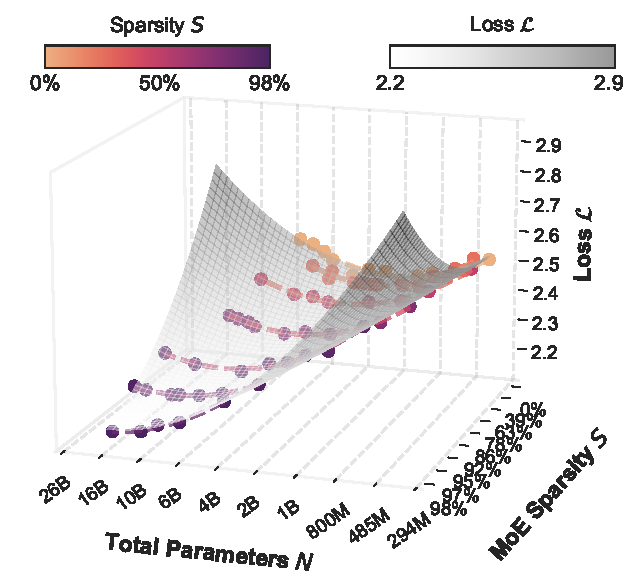
\includegraphics[width=0.45\textwidth]{plots/3d_suface_fit_total_params.pdf}
    }
    \quad %\hfill
    \subfigure[IsoFLOP surface over sparsity and active parameters]{
        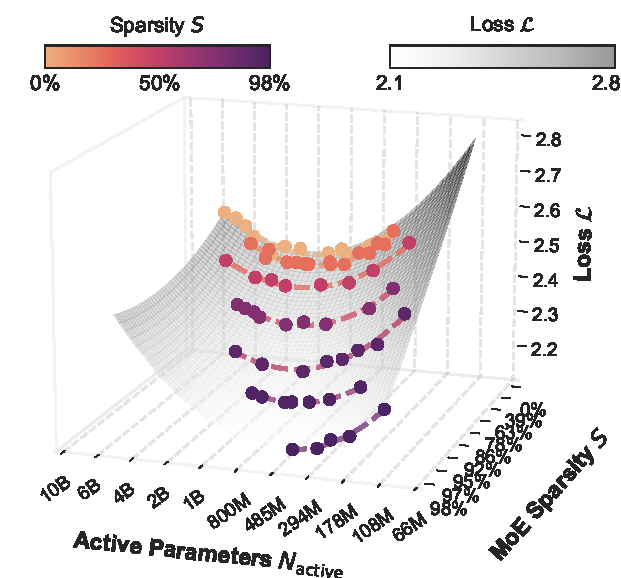
\includegraphics[width=0.45\textwidth]{plots/3d_suface_fit_active_params.pdf}
        \label{fig:iso_surface_active}
    }
    \caption{\textbf{IsoFLOP surface over observed pretraining loss $\mathbf{L}$, model size (in terms of total $\mathbf{N}$ and active parameters $\mathbf{N_a}$), and sparsity $\mathbf{S}$.} We fit a polynomial function mapping $\mathbf{N}$ (or $\mathbf{N_a}$), $\mathbf{S}$, and their interaction to $\mathbf{L}$, using empirical data. For both fits the MSE loss for predicting loss on a held out set is $0.0001$. These results indicate that for a fixed compute budget, increasing model sparsity leads to a reduction in pretraining loss. When considering optimal model size, we observe opposite trends for total parameters ($\mathbf{N}$) (Figure a) versus active parameters ($\mathbf{N_a}$) (Figure b). (See \Cref{fig:additional_surfaces} in \Cref{app:n_s_d_interaction} for results with different total compute budgets $C$.)}
    \label{fig:iso_surface}
\end{figure*}


When studying scaling laws for specific classes of models, e.g., vanilla transformers, the total number of parameters can serve as a reasonable relative estimator of \flops per example. 
Therefore, using the number of parameters as a measure of model capacity in scaling law studies is appropriate. 
In scenarios or for architectures where the number of parameters and \flops per example are not directly linked, it is essential to jointly consider the effects of these variables on scaling model capacity~\citep{clark2022unified}.
We therefore ask
\begin{center}
\emph{``Can we draw scaling laws for the optimal trade-off between\\parameter count and \flops per example?''} 
\end{center}
To address this question, we study sparse Mixture-of-Expert Transformers (\moes)~\citep{shazeer2017,lepikhin2021gshard,fedus_switch,zoph2022st,muennighoff2024olmoe} in the context of language modeling.
Existing scaling law studies for \moes, investigate the role of variables like number and granularity~\citep{ludziejewski2024scaling} of experts, underlying dense model size and inference compute in predicting the performance of the models under different conditions such as training or inference compute optimality~\citep{Du2021GLaMES,clark2022unified,yun2024toward,ludziejewski2024scaling}. In this paper, we focus on the interaction between \flops per example and total parameter count, and their impact on model performance in \moes, through a large-scale empirical study. 

 
We define sparsity as the ratio of inactive experts to the total number of experts, which controls the ratio of the total number of parameters to \flops per example in \moes. We evaluate loss and downstream metrics for different sparsities, model sizes, and compute budgets.
Through qualitative and quantitative analysis to derive scaling laws which disentangle total parameters vs \flops per example in \moes, we can estimate the optimal sparsity level under the setting where both total training \flops and total number of parameters are given and fixed. Generally, we find that:
\begin{itemize}

\item During pretraining, increasing a model’s capacity by adding more parameters yields greater benefits than increasing \flops per example. We observe that the size of compute-optimal models increases as we increase the training budget (measured in terms of total \flops) while the active number of parameters, hence \flops per example, decrease for compute-optimal models.

\item During inference, \flops per example seem to play a more important role\footnote{A relevant discussion here is the recent trend of increasing test-time compute, e.g., OpenAI o1 model~\citep{openai2024openai}, achieved by generating more tokens as a way for introducing parameter-free-FLOPs.}.
For many tasks, upstream performance is a good predictor of downstream performance and the relationship between upstream and downstream performance is not impacted by the sparsity level. However, on downstream tasks that presumably require more ``reasoning'', we observe that for models with the same perplexity on the pretraining data distribution, sparser models, i.e., models with fewer active parameters, perform worse. 
\end{itemize}


Our results, in line with findings from previous relevant studies~\citep{ludziejewski2024scaling,he2024mixture} on scaling laws for \moes, show increasing sparsity level leads to better performance and efficiency during pretraining. 
Considering the various methods to increase compute per example during inference adaptively conditioned on task or example complexity, we conclude that approaches like \moes, which reduce the unit compute cost (i.e., FLOPs per token) by increasing the sparsity level, hold significant promise given their potential to enhance efficiency in both pretraining and inference.

% \input{sections/setup}
\begin{figure*}[ht]
    \centering
    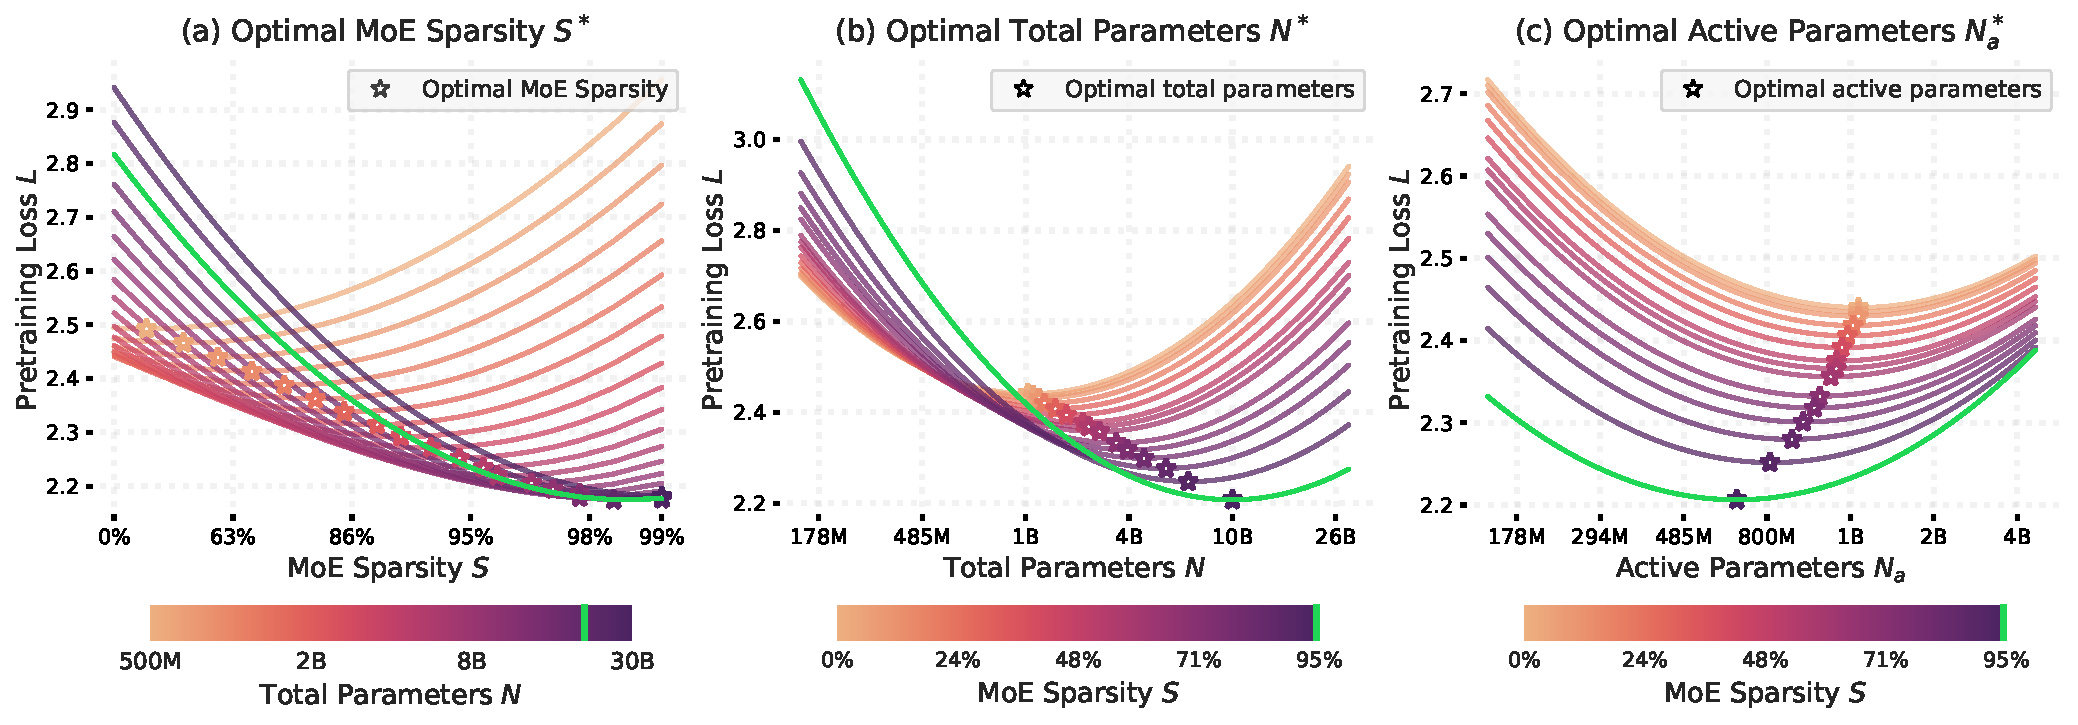
\includegraphics[width=0.95\textwidth]{plots/v2_s2_plot2_logS_colorbar_tickfix.pdf}
    \caption{\textbf{IsoFLOP slices along Sparsity and Model Size ($C=1e20$).}
    We use fitted isoFLOP surfaces (\Cref{sec:n_s_d_interaction}) to analyze how sparsity $\mathbf{S}$ and model size $\mathbf{N}$ impact the loss $\mathbf{L}$ for a fixed compute budget. We identify optimal points by (a) fixing $\mathbf{N}$ and varying $\mathbf{S}$, (b) fixing $\mathbf{S}$ and varying $\mathbf{N}$ and (c) fixing $\mathbf{S}$ and varying active parameters $\mathbf{N_a}$.  Observe that (a) the optimal sparsity $S$ increases with increasing model size $N$ and converges to 1 while (b) and (c) show that the optimal model size $N$ and active parameter count $N_a$ increase and decrease respectively with increasing sparsity levels. (see \Cref{fig:additional_surface_eval} in \Cref{app:n_s_d_interaction} for other total
training compute budgets.)
    \label{fig:iso_surface_sliced}
    }
\end{figure*}

\section{The Interplay between Model Parameters and Sparsity in \moes}
\label{sec:n_s_d_interaction}

Is there an optimal trade-off between parameter count and \flops per example in \moes under the setting where the training compute budget (i.e., total training \flops) is fixed?



Intuitively, under infinite data setting, scaling  model capacity along with the training compute budget leads to performance improvements. 
Previous scaling law studies suggest that, conditioned on a training compute budget measured in \flops denoted by \(C\), the optimal number of parameters, \(N^*(C)\), exhibits a power-law relationship with \(C\)~\citep{hoffmann2022training}:
\begin{equation}
    N^*(C) = \arg\min_{N} \mathcal{L}(N;C) \propto C^{a}
    \label{eqn:loss_n}
\end{equation}
Our goal is to study how to optimally trade-off \flops per example and total parameters in \moes.
In \moes the balance between parameters and \flops can be expressed through the sparsity level, $S$. We define $S$ as the ratio of non-active to total number of experts, i.e., $S = \frac{E - K}{E}$; where $E$ is the total number of experts and $K$ is the number of selected  experts per token. We can vary the sparsity level by either changing the number of active experts $K$ or total number of experts $E$.
\footnote{Sparsity level determines the number of active parameters given the total number of parameters and we use the active number of parameters as a proxy for \flops per example, as \( 6N_aD \) provides a good estimate of the total FLOP count for MoEs; see~\Cref{app:train_inference_cost} for details.}
Essentially, for models with the same \( N \), the model with a higher \( S \) will have fewer active parameters \( N_a \), resulting in fewer \flops per example. For more details on the notations and experimental settings see \Cref{app:prelim} and \Cref{app:exp_setup}.


\begin{equation}
    (N^*, S^*) = \arg\min_{N,S} \mathcal{L}(N,S;C)
    \label{eqn:optimal_ns_given_c}
\end{equation}

To simplify the problem of understanding the joint role of \( N \) and \( S \) in predicting \( L \), we break the problem, \Cref{eqn:optimal_ns_given_c}, into two parts:
\begin{enumerate}[left=0pt,itemsep=2pt]
\item \textit{"How does the sparsity level impact the scaling laws of the relationship between \( N \) and \( C \) for training-compute optimal models?"}
To address this question in \S\ref{sec:fix_sparsity_vary_params}, we fix \( S \) and vary \( N \), studying how optimal \( N \) and \( N_a \) change for different values of \( S \):
\begin{equation}
    N^* = \argmin_{N} \mathcal{L}(N; C, S)
\label{eq:fix_sparsity_vary_N}
\end{equation}
\item \textit{"Is there an optimal balance between total number of parameters and the sparsity level under fixed training-compute budget?"}
To address this question in \S\ref{sec:fix_params_vary_sparsity}, we fix \( N \) and vary \( S \), studying how optimal \( S \) changes across different values of \( N \):
\begin{equation}
    S^* = \argmin_{S} \mathcal{L}(S; C, N)
\label{eq:fix_N_vary_sparsity}
\end{equation}
\end{enumerate}
As the first step, considering a fixed training compute budget \( C \), we fit a 3D surface, referred to as the IsoFLOP surface, in \Cref{fig:iso_surface}a, using a polynomial function, following approach II of \citet{hoffmann2022training}. 
Compared to \citet{hoffmann2022training} we include the sparsity variable and fit a single 3d IsoFLOP surface across all data points, rather than fitting separate 2d IsoFLOP curves for fixed sparsity levels or model sizes. 
We conducted a grid search to determine the optimal polynomial degree for \( N \), \( S \), and the interaction term \( N \times S \), finding that a degree of \( (2, 2, 2) \) resulted in the lowest cross-validation error. Both \( N \) and \( S \) are in log space (see \Cref{app:exp_setup} for more details).

As seen in \Cref{fig:iso_surface}a, the IsoFLOP surface plot is parabolic along model size, suggesting that the findings of \citet{hoffmann2022training} extend to MoEs across different sparsity levels, i.e., \( \mathcal{L}(N; C, S) \) is parabolic, with its optimal solution located at the turning point. When considering the total number of parameters $N$, the optimal value increases as the sparsity level increases, while for the active number of parameters $N_a$ the optimal value decreases with the sparsity level. This indicates that by increasing the sparsity level the training compute optimal models are larger but have fewer \flops per example, i.e., lower inference cost. 
Moreover, along sparsity, the pretraining loss decreases monotonically, indicating that, for the same compute budget, sparser models achieve better pretraining performance. We observe the same pattern across different training compute budgets (See \Cref{app:n_s_d_interaction}). To better understand and explain these observations, we examine slices of the IsoFLOP surface along the axes of \( S \) and \( N \) separately in \S\ref{sec:fix_sparsity_vary_params} and \S\ref{sec:fix_params_vary_sparsity}, respectively.

\subsection{Optimal Model Size for Fixed Sparsity Level}
\label{sec:fix_sparsity_vary_params}

Here we examine how sparsity influences scaling laws governing the relationship between \( N \), \(N_a\) and \( C \) for training-compute optimal models, i.e. how does \( N^* \) and \( N_a^* \), for a given $C,S$ 
(\Cref{eq:fix_sparsity_vary_N}), change as we increase \( S \)?
Looking at slices of the IsoFLOP surface along the model size dimension, in \Cref{fig:iso_surface_sliced}b and \Cref{fig:iso_surface_sliced}c, we observe how the IsoFLOP curves shift along loss and model size. 
Considering the training-compute optimal model, for a fixed compute budget, loss decreases as we increase sparsity. Furthermore, while sparser models have larger \( N \) compared to denser models, as seen in \Cref{fig:iso_surface_sliced}b, they have a smaller active parameter count \( N_a \); hence, fewer FLOPs per example. Intuitively, more parameters in total increase the capacity of the sparser models to fit the data, while fewer number of active parametes, hence fewer \flops per example, allow the model to be trained with more tokens, i.e., higher \( D \), for the same training compute budget. 

\subsection{Optimal Sparsity Level for Fixed Model Size}
\label{sec:fix_params_vary_sparsity}
In this section we aim to understand the dynamics between the total number of parameters and \flops per example in \moes. 
In \Cref{sec:fix_sparsity_vary_params} we are considering the case where there is no bound on the total number of parameters. In this case, we observe that under fixed training  compute budget in terms of \flops, it is better to train  sparser models with higher total number of parameters. However in practical scenarios it is reasonable to assume that there would be some bounds on the memory and hence the total number of parameters of a model. 
This leads us to a fundamental question: Is there an optimal balance between the total number of parameters and and \flops per example under a fixed training-compute budget? 
Thus, we investigate the optimal sparsity level when total number of parameters is fixed.
Specifically, we ask: Given \(N\) and \(C\), How does \(S^*\) change as we vary \(N\)?

To address this, we look into slices of the IsoFLOP surface along the sparsity dimension. As we can see in \Cref{fig:iso_surface_sliced}a, for a fixed training compute budget and fixed model size $\mathcal{L}(S; N,C)$ exhibits a parabolic profile, reaching its optimum value at the vertex where $S = S^*$. It is noteworthy that for a given total training compute, there is threshold value $N_{th}$ for the total number of parameters, where for larger models, models with \( N > N_{th} \), increasing sparsity always has a positive impact, i.e., optimal sparsity level approaches $1.0$. More accurately, for a fixed compute budget the optimal sparsity level increases with model size and converges to $1$ as the model size grows (see \Cref{fig:opt_sparsity} in \S\ref{app:budget} in the Appendix for more details).
Note that the optimal model, here is not the largest model, i.e., there is a compute optimal model size in terms of total parameters even after sparsity is introduced, and increasing total number of parameters would lead to under-training if training compute budget is fixed.

These results highlight the importance of balancing the number of parameters with \flops per example in \moes. Intuitively, when the total number of parameters is small, higher sparsity results in fewer active parameters, and thus fewer \flops per example. This reduction in \flops per example may lead to inefficiencies during both training and inference. Conversely, when the total number of parameters is large, for a reasonable amount of \flops per example, a fixed compute budget may not allow sufficient training on enough tokens to make use of the model's additional capacity.

\begin{figure*}[t]
    \centering
    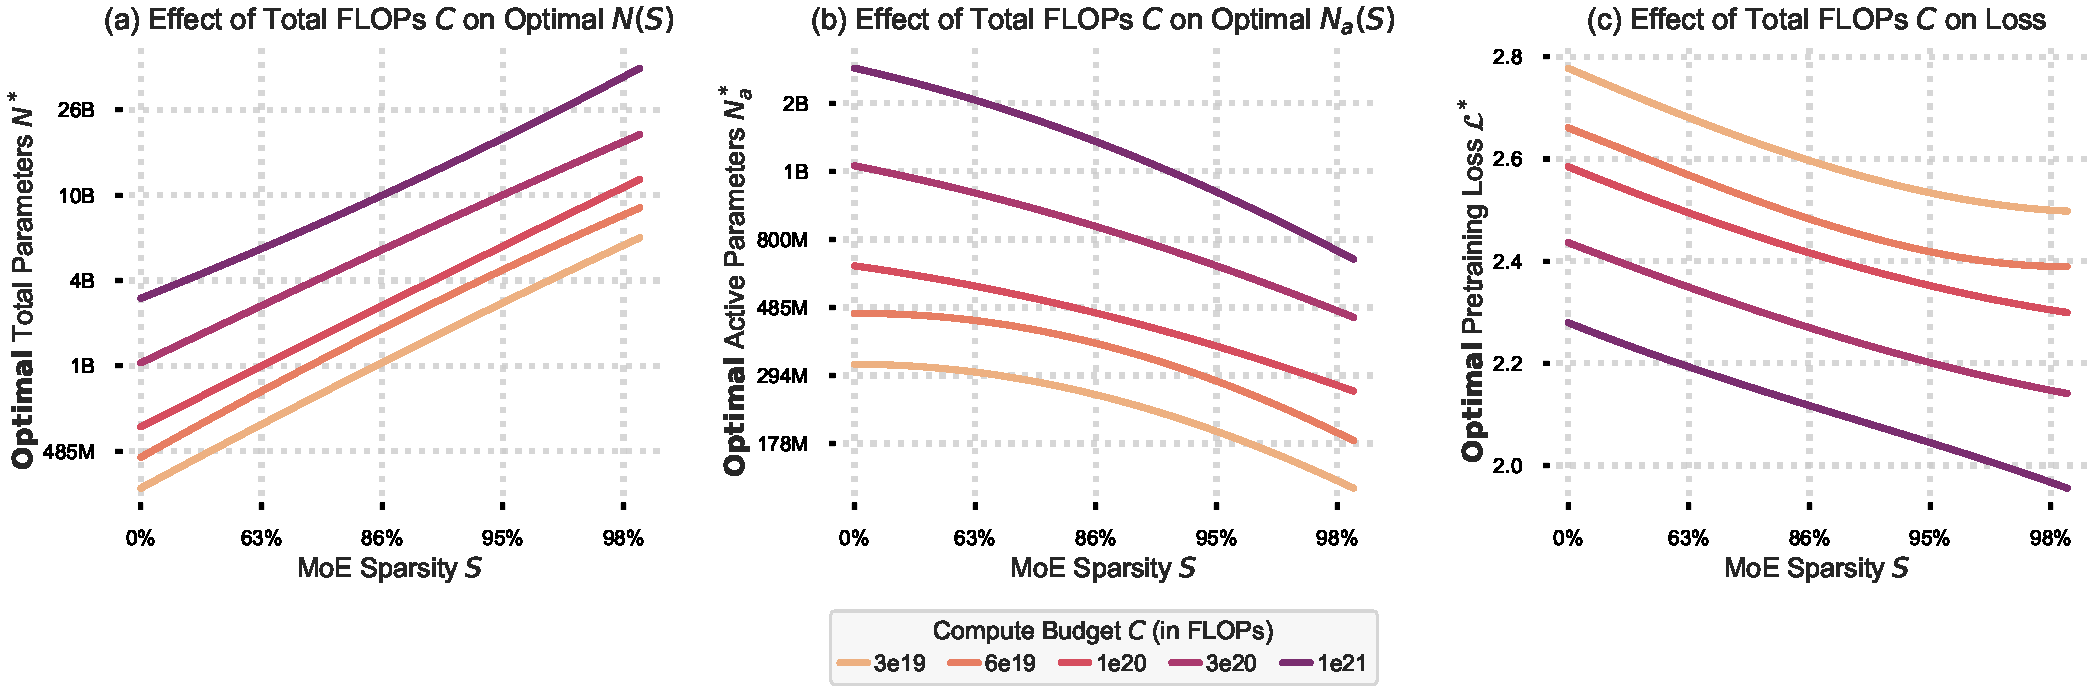
\includegraphics[width=0.8\textwidth]{plots/effect_of_total_flops_on_optimals.pdf}
    \caption{
    \textbf{Effect of compute budget on model size, number of active parameters and loss with sparsity.} Across all compute budgets, we observe that (a) the optimal model size $N$ increases with sparsity, (b) the optimal number of active parameters $N_a$ decreases with sparsity, and (c) the loss $L$ decreases with sparsity. 
    % We can see that larger models get sparser and have better performance at 
    % . (a) depict how optimal \( N \) increase with sparsity with a similar slope across different training compute budgets. (b) shows how optimal \( N_a\) decreases with sparsity across different sparsity levels. (c) shows how the loss for the compute optimal model decreases with sparsity across different compute budgets.
    % \Harshay{reminder to update plot if we decide to remove 1e21}
    }
    \label{fig:effect_of_compute}
    \vspace{-0.3cm}
\end{figure*}


\section{Impact of Training Compute Budget on the Interaction between Model Parameters and Sparsity} 
\label{sec:effect_of_training_budget}

Does increasing compute budget impact the interaction between the parameters and \flops per example in \moes and how they contribute to model's capacity?
In other words, does the recipe for optimally increasing model capacity, i.e., optimal sparsity level for \moes change as we scale up the total training compute? 

To answer this question. in \Cref{fig:effect_of_compute} we illustrate the trends for changing the total number of parameters, $N^*$, the number of active parameters, $N_a^*$, and the loss, $L^*$, with sparsity level across different compute budgets. 

\Cref{fig:effect_of_compute}c shows that the optimal sparsity level approaches 1 across all compute budgets used in our experiments. There is no significant difference observed in the slope of the loss vs sparsity curves across different training compute budgets used in our experiments. 
This observation suggests that there is no diminishing effect of sparsity on the pretraining loss as we increase training compute budget, i.e., if there is no constraint on the model size, sparsity improves the performance of the model across all training budgets.


In \Cref{fig:effect_of_compute}a and \Cref{fig:effect_of_compute}b, , we see a consistent trend of increasing \( N\) and decreasing \( N_a \) for compute optimal models as sparsity level increases across all training compute budgets.
Moreover, as can be seen in \Cref{fig:opt_sparsity}, when model size in terms of total number of parameters is fixed,  optimal sparsity level decreases with training compute budget while increases with model size as discussed in \Cref{sec:fix_params_vary_sparsity}.

\ifthenelse{\boolean{@twocolumn}}{
\begin{figure}
    \centering
    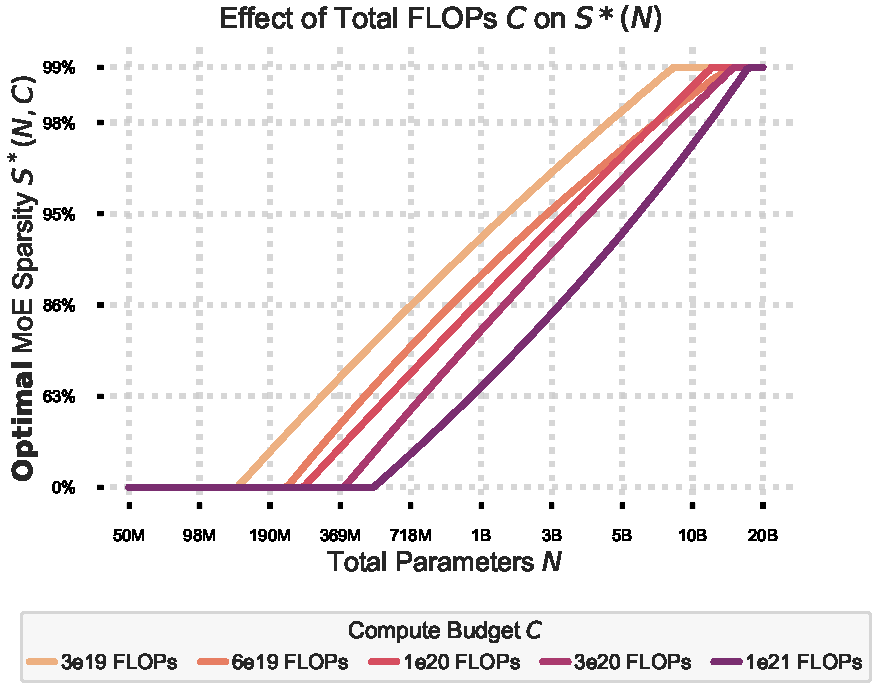
\includegraphics[width=0.45\textwidth]{plots/optimal_sparsity.pdf}
    \caption{\textbf{Effect of training budget $C$ and total parameters $N$ on MoE sparsity.} Optimal MoE sparsity $S^*$ changes with respect to the total number of parameters $N$ and the training budget $C$. The $x$-axis represents the total parameters $N$ on a logarithmic scale, and the $y$-axis shows the optimal MoE sparsity $S^*$.}
    \label{fig:opt_sparsity}
\end{figure}
}
{
\begin{wrapfigure}{r}{0.5\textwidth}
    \centering
    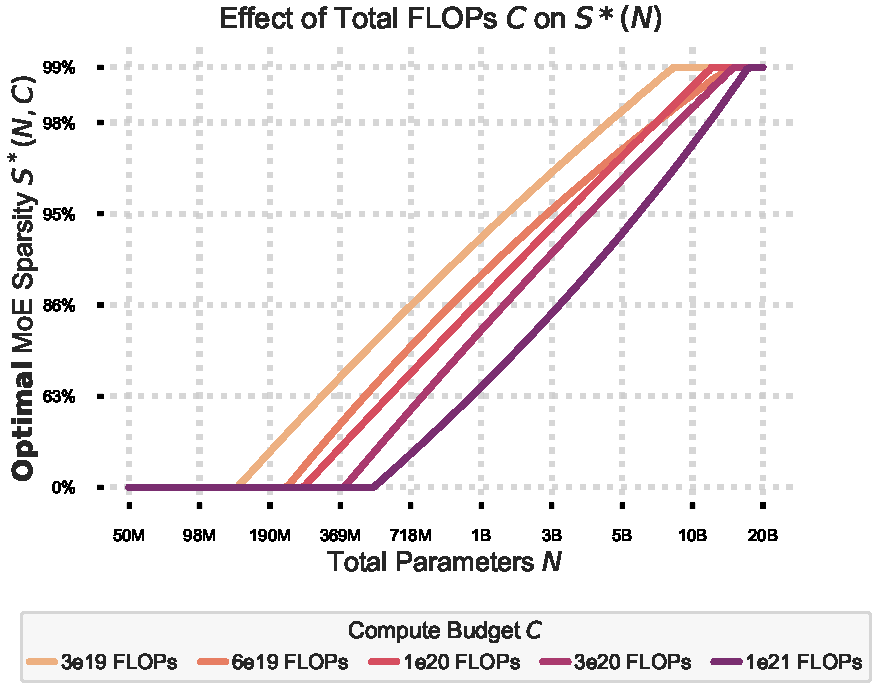
\includegraphics[width=0.45\textwidth]{plots/optimal_sparsity.pdf}
    \caption{\textbf{Effect of training budget $C$ and total parameters $N$ on MoE sparsity.} Optimal MoE sparsity $S^*$ changes with respect to the total number of parameters $N$ and the training budget $C$. The $x$-axis represents the total parameters $N$ on a logarithmic scale, and the $y$-axis shows the optimal MoE sparsity $S^*$.}
    \label{fig:opt_sparsity}
\end{wrapfigure}}

%  However, the rate of decreasing \( N_a \), which can be interpreted as inference cost, increases as we increase training compute budget. This means, at larger training compute budgets, the benefit of reducing compute in terms of FLOPs per example amplifies. i.e., the gains of increasing sparsity level to reduce inference cost becomes more significant at larger training budgets. 


% As the compute budget increases, the optimal sparsity level decreases for a fixed model size, while the expected optimal model size increases—both in terms of total parameters and active parameters. 





\section{Effect of \moe Sparsity on Downstream Task Performance}
\label{sec:scaling_law_ds}
In this section, we study how sparsity affects the relationship between upstream and downstream performance of \moes. In other words, does sparsity impact the relative gains from improvements in pretraining tasks on downstream tasks?

We use downstream tasks from the evaluation suite in~\texttt{llm-foundry}\footnote{Github repository: \url{https://github.com/mosaicml/llm-foundry}} for benchmarking our pretrained models, specifically in an in-context few-shot learning setup. This setup focuses on evaluating a model's ability to learn and adapt to new tasks with limited examples.
The downstream task are devided into four pre-defined categories namely: language understanding, world knowledge, reading comprehension, and symbolic reasoning to help us systematically test whether the downstream vs upstream performance trend remains the same or is different as we vary sparsity values.

\begin{figure*}[!t]
    \centering
    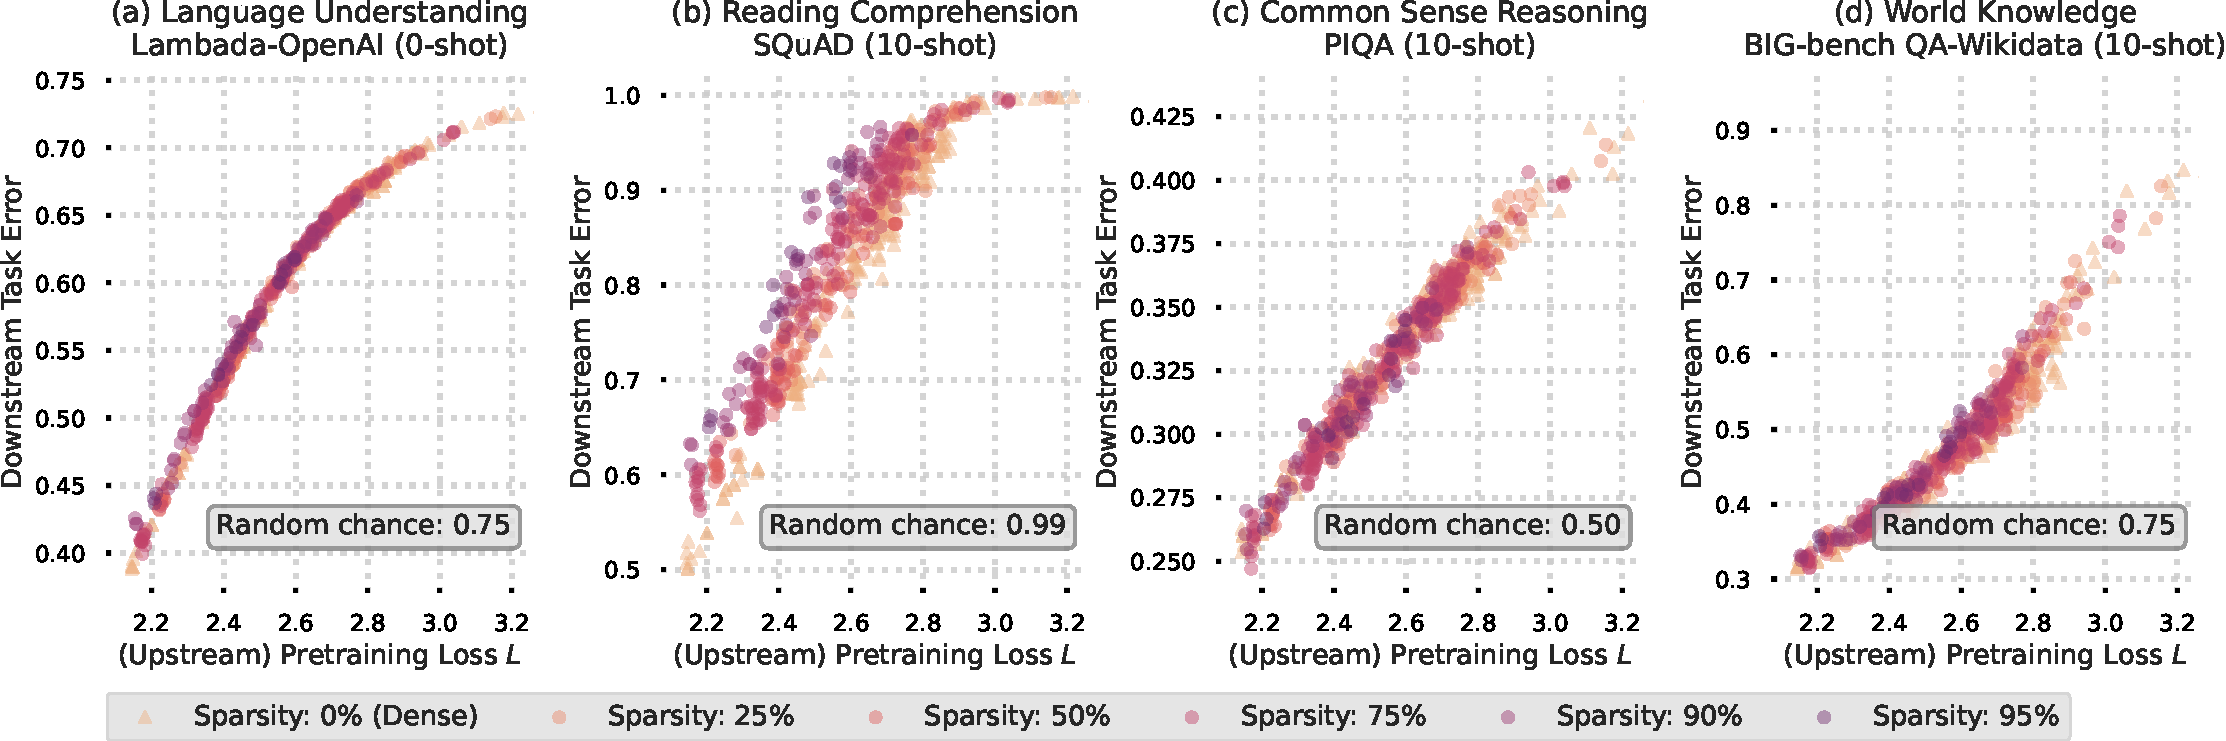
\includegraphics[width=0.95\textwidth]{plots/s4_plot.pdf}
    \caption{
    \textbf{Effect of sparsity on downstream vs upstream performance.} Downstream error shows a tight relationship with pretraining (``upstream'') loss across downstream tasks across all sparsity levels. 
    }
    \label{fig:downstream}
\vspace{-15pt}
\end{figure*}

We observe from ~\Cref{fig:downstream}a (language understanding), ~\Cref{fig:downstream}c (commonsense reasoning), and ~\Cref{fig:downstream}d (world knowledge) that, in an in-context few-shot learning setting, there is a strong correlation between upstream (pretraining) loss and downstream performance (error) across all these tasks. For these tasks, downstream performance in the few-shot setting is predictable based on upstream performance, regardless of the sparsity level. This indicates that, in the context of these tasks, the optimal sparsity level follows the same trend as the optimal sparsity observed during pretraining.
%Furthermore, \moes downstream performance improve with increasing sparsity levels. 
However,~\Cref{fig:downstream}b (reading comprehension) shows an example of a task where models with higher sparsity transfer more poorly compared to denser models. This decrease in the transfer performance of sparser models on these tasks may be due to the lower inference-time compute in sparser models compared to their denser counterparts for a similar pretraining loss. Further analysis is needed to verify this intuition. 

If fewer \flops per example are the reason behind the worse transfer performance in sparser models, this effect might diminish with a larger total training compute budget, as the optimal active number of parameters increases. Moreover, one can use approaches like chain-of-thought reasoning~\citep{wei2022chain_cot} to independently increase \flops per example during inference time. 

In \Cref{app:cot_expt}, we explore whether increasing inference-time compute via Chain-of-Thought (CoT) prompting can improve the performance of MoEs on tasks that require more reasoning. Our experiments indicate that MoEs benefit more from this increased compute compared to dense models with a similar number of active parameters. This suggests that dynamic compute allocation during inference may be crucial for MoEs to perform well on complex reasoning tasks.

While our results may indicate that there may be no additional benefit obtained via sparsity in \moes beyond the efficiency gains for pretraining, we caution the reader that this suggestion may be an artifact of the scale of our experiments. In the end, since, as shown in \S\ref{sec:n_s_d_interaction}, sparser models are more efficient both in terms of training and inference cost (when measured in terms of theoretical \flops), we can reach better pretraining performance with higher sparsity levels at a lower cost, which can translate to better downstream performance.

% Better pretraining performance can be achieved with increased sparsity without sacrificing either training or inference cost (when measured in terms of theoretical \flops).

% We observe that for tasks in the categories of language understanding, an example of which is shown in~\Cref{fig:s4}a, and world knowledge, ~\Cref{fig:s4}d, there is a tight relationship between upstream and downstream performance, i.e., a model with a low pretraining loss also has a low downstream error. Furthermore, models performance improve with sparsity.

% Interestingly, for tasks that fall into the reading comprehension category, an example of which is shown in~\Cref{fig:s4}b, sparsity seem to have a negative effect, i.e., given two models with the same pretraining loss, a denser model is more likely to have a lower downstream error.  
% Intuitively, a reason behind this could be that denser models use more compute during inference as they have higher number of active parameters. This suggests that methods like chain of thought reasoning could potentially help close the gap as we increase the sparsity level of models. We defer further investigation of this hypothesis to future work.

% TODO complete the following
% These results suggest that \moes with higher sparsity levels show improved performance over their lower sparsity counterparts. However, the results do not suggest that \moes unlock additional capability in the downstream tasks considered in our work

% These results suggest, there is no significant additional benefit when introducing sparsity in \moes for transfer, at the current scale of our experiments. Since, as shown in section~\ref{}, sparser models are more efficient both in terms of training and inference cost (when measured in terms of theoretical \flops), we can reach a better pretraining performance with sparser models at a lower cost. Hence, sparser models are generally more favorable. \todo[inline]{need a better way to phrase this.}

% To further confirm this, in Figure~\ref{}, we show how DS performance changes as a function active number of parameters (proxy for inference cost) and training compute budget. We observe that ...
% \todo[inline]{what exactly do we want to plot to summerize the message}.

% Previous studies have shown ...


% Scaling law for predicting DS loss fiven US loss (perplexity on the pretraining data), when architecture and pretraining data are fixed:
% \begin{equation}
% L(DS) = k \cdot L(US)^{\alpha} + e
% \label{eq:ds_us_scaling}
% \end{equation}

% First, we fit this equation for dense models as well as models with different sparsity levels. We investigate weather the sparsity level impact the scaling law co-efficents for predicting DS perfomrance from US performance. 

\section{Incorporating Sparsity into Scaling Laws}
\label{sec:deriving_scaling_laws}
The scaling laws proposed by \citet{kaplan_scale} provide a framework for predicting loss in dense models by establishing a power-law relationship between loss \(L\), number of parameters \(N\) and dataset size \(D\), where \(N\) and \(D\) interact linearly. Formally, the relationship is given by:
\begin{equation}
L(N, D) = \frac{a}{N^{\alpha}}  + \frac{b}{D^{\beta}} + e
\label{eq:loss:dense}
\end{equation}
Here, the term \(N^{\alpha}\) captures the inverse relationship between model size and loss, where an increase in model size \(N\) leads to a reduction in loss. The exponent \(\alpha\) quantifies the rate of this decrease; a larger \(\alpha\) suggests a steeper reduction in loss with increasing model size. Similarly, the term \(D^{\beta}\) indicates the impact of dataset size \(D\) on loss, with larger datasets contributing to lower loss values. The exponent \(\beta\) measures this relationship, where a larger \(\beta\) implies a greater benefit from increased data. The constant \(e\) represents an asymptotic minimum for the loss, as both model size and dataset size approach infinity.


For dense models with a fixed total training \flops, \(C\), the parameters \(N\) and \(D\) are interrelated through the equation for estimating \flops per example, given as \(C = 6ND\) for transformers.
However, in \moes (Mixture of Experts models), this relationship involves the active number of parameters \(N_a\) rather than the total parameter count \(N\). Thus, \(D\) and \(N_a\) define the total training \flops rather than \(D\) and \(N\).
Given the analysis conducted in \S\ref{sec:n_s_d_interaction}, we know that if the total number of parameters $N$ is fixed, the optimal sparsity level, i.e., active number of parameters would depend on $N$. Motivated by this observation, we suggest the following parametric form  that includes a multiplicative interaction between $N$ and $S$ or $N_a$ to predict the loss:

\begin{equation}
    L(N, D, S) = \frac{a}{N^{\alpha}}  % c, \lambda in NB
                + \frac{b}{D^{\beta}}
                + \frac{c}{\left(1-S\right)^{\lambda}}  % a, \alpha in NB
                + \frac{d}{\left(1-S\right)^{\delta}N^{\gamma}}
                + e
    \label{eq:loss:moe:proposal1}
\end{equation}
The term $\left(1-S\right)$ in the above equation provides a rough estimate of the percentage of active parameters. If the exponent for the multiplicative terms is the same then that term provides an approximate estimate of the number of active parameters.

By incorporating sparsity into the scaling law equation, we can eliminate the need for parameters specific to \moes, such as the total and active number of experts. As demonstrated by \citet{frantar2024scaling}, this formulation also holds for other sparsity mechanisms, such as weight sparsity, where individual neural network connections are pruned.

We use the recipe described by~\citet{hoffmann2022training} and use the L-BFGS algorithm to fit the coefficients in~\eqref{eq:loss:moe:proposal1} using a Huber loss with $\delta=10^{-3}$. Optimal coefficient values were determined through a grid search (see \Cref{tab:lbfgs:hparams} for search values). The results of data fitting and validation are shown in~\Cref{fig:scaling_law}. The estimated values are shown in~\Cref{tab:lbfgs:estimate_params} in~\Cref{appendix:scaling_law_sparsity}. 

\begin{figure*}[ht]
    \centering
    \subfigure[Fit on data used to estimate coefficients.]{
        \label{fig:scaling_law:interpolation}
        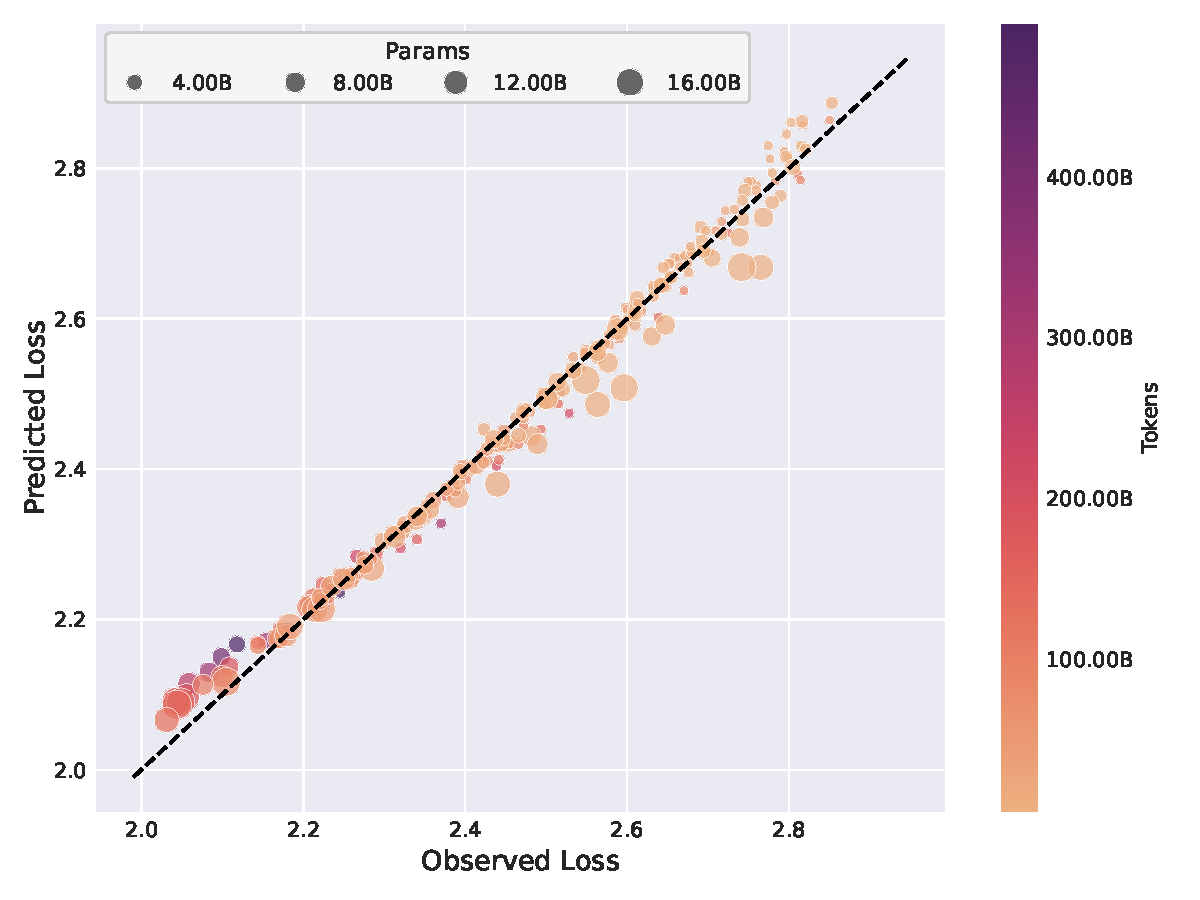
\includegraphics[width=0.45\textwidth]{plots/parameteric_law_interpolation.pdf}
    }
    \quad %\hfill
    \subfigure[Validating scaling law on held-out dataset.]{
        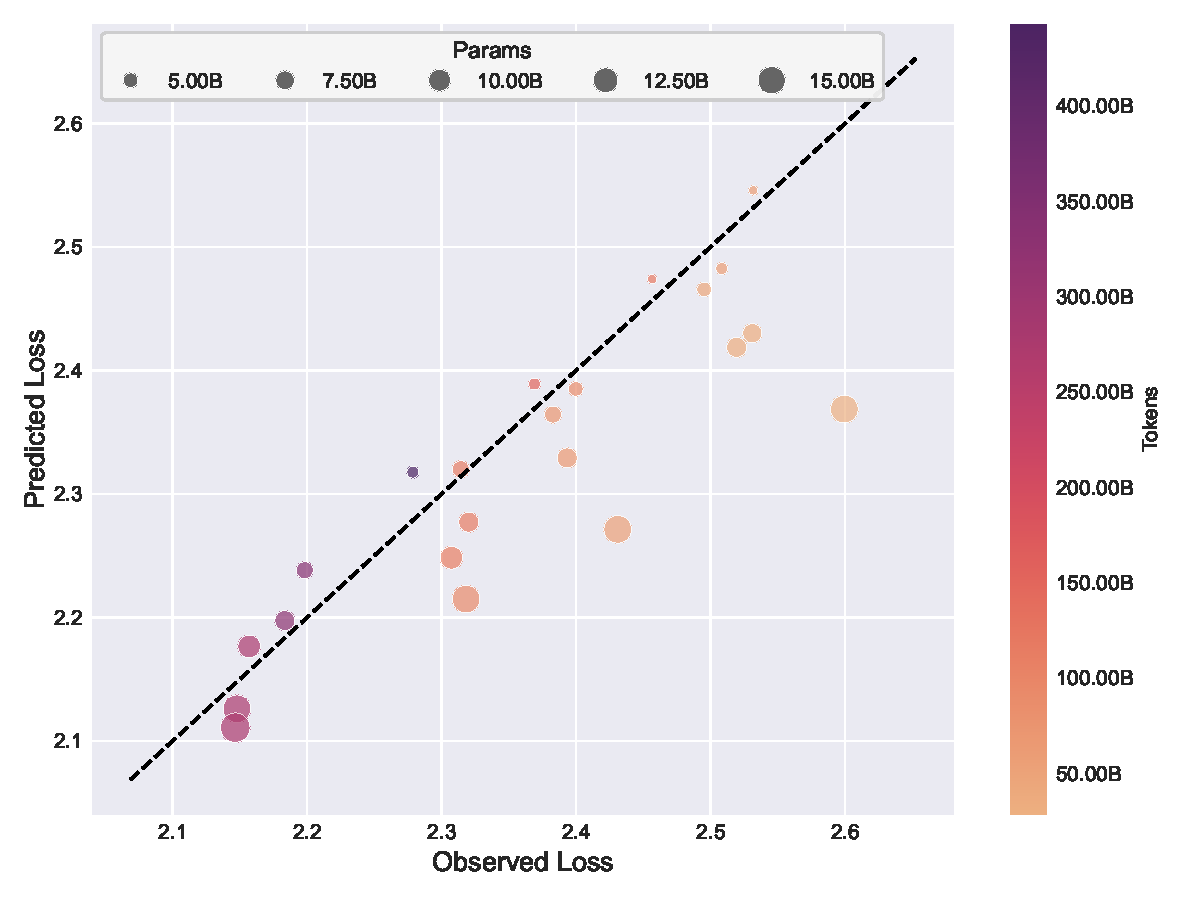
\includegraphics[width=0.45\textwidth]{plots/parameteric_law_extrapolation.pdf}
        \label{fig:scaling_law:sparsity98}
    }
    \caption{Scaling law fit on data obtained from training compute-optimal models. \Cref{fig:scaling_law:interpolation} shows the fit on the data used to estimate the coefficients for \eqref{eq:loss:moe:proposal1}, while \Cref{fig:scaling_law:sparsity98} validates these coefficients on a held-out dataset. All data points with \(S = 0.98 \) were excluded from the fitting process for out-of-sample validation.  The dashed lines represent equal loss values.}
    \label{fig:scaling_law}
\end{figure*}


\section{Discussion}
\label{sec:discussion}
Our findings amplify the findings of \citet{ludziejewski2024scaling} and further justify the effort to work toward \moes with experts larger in number and smaller in size~\citep{he2024mixture}. For downstream tasks which their performance is predictable given the pretraining loss (i.e., perplexity), sparsity potentially provides efficiency gains both during pretraining and inference. 

Here is a summary of our observations as discussed in \Cref{sec:n_s_d_interaction,sec:effect_of_training_budget,sec:scaling_law_ds,sec:deriving_scaling_laws} :
\begin{itemize}[leftmargin=*]
    \item \textbf{Larger, Sparser Models Perform Better under a Fixed Compute Budget:} When memory and communication overheads are disregarded, increasing sparsity while proportionally expanding the total number of parameters consistently leads to a lower pretraining loss, even when constrained by a fixed training compute budget (see \S~\ref{sec:n_s_d_interaction}).

        \item \textbf{Optimal Sparsity for Fixed Model Size:} 
    For any given number of parameters and under a fixed training compute budget, model performance as a function of sparsity exhibits a parabolic pattern, reaching its peak at an optimal sparsity level (see \S\ref{sec:fix_params_vary_sparsity}). Specifically, the optimal sparsity level:
    \begin{itemize}
        \item Increases with the total number of parameters approaching $1.0$ for larger models. i.e., if a model is relatively small for a given training compute budget, sparsifying it more than a threshold will hurt its performance. On the other hand, if a model is relatively large for a given compute budget, further sparsifying it helps as it leads to increase in the number of tokens the model is trained on under the given training budget constraints (see \S\ref{sec:fix_params_vary_sparsity}). 
        \item Increases across all model sizes as the training compute budget increases (see \S\ref{app:n_s_d_interaction} and \S\ref{app:budget}). 
    \end{itemize}
    
    \item \textbf{Effect of Sparsity on Scaling Laws for Optimal Model Size:} For any specific sparsity level, performance of the models as a function of their size exhibits parabolic behavior under a fixed training compute budget. i.e., the model reaches its optimal performance at a vertex, that indicates optimal model size.
    Under these conditions:
     \begin{itemize}
     \setlength{\itemindent}{0pt}  % No extra indentation for items
     \setlength{\leftmargin}{0pt}  % No left margin
      \item The optimal active number of parameters decreases as the sparsity level increases, leading to smaller \flops per example and more efficient inference even though the total number of parameters increases (see \S\ref{sec:fix_sparsity_vary_params}).
      \item While the trend of increasing active number of parameters is similar across all training compute budgets; the optimal active number of parameters decrease more rapidly with sparsity as the training compute budget increases (see \S\ref{sec:effect_of_training_budget}). 
\end{itemize}
    \item \textbf{Effect of Sparsity on Downstream Performance:} For most downstream tasks, models with similar pretraining perplexity have similar downstream task performance regardless of sparsity. For reading comprehension tasks (e.g., CoQA~\citep{reddy-etal-2019-coqa}, SQuAD~\citep{rajpurkar-etal-2018-know}), denser models perform better, potentially due to their higher inference-time compute than a perplexity-matched sparse model. Strategies to increase inference time compute dynamically~\citep{wei2022chain_cot,goyal2024think_pause} may address this gap. 
    % We use a ``length-controlled'' variant of few-shot Chain-of-Thought (CoT) prompting to study whether this strategy may help close the gap between \moes and dense models on reasoning tasks in~\Cref{app:cot_expt}. Empirical evidence suggests that \moes may benefit more from dynamically increased inference-time compute than dense models under a fixed generated tokens budget. 

    \item \textbf{Parametric Scaling Law:} We propose a parametric form for scaling laws that accounts for sparsity. The model coefficients are estimated using the empirical data obtained by training compute-optimal models. An interesting observation from ~\Cref{appendix:scaling_law_sparsity} is that the exponent for sparsity term $\lambda$ is negative which is consistent with our intuition that sparser models lead to a lower perplexity. 
\end{itemize}

%How increasing the sparsity level makes pretraining more efficient?
% Based on these observations, during pretraining, sparsity allows us to increase the model capacity by adding more parameters, while at the same time increasing the amount of data the model sees with the the same total training flops by reducing the number of \flops per token. 

% %How we can benefit from reduced flops per example during inference? 
% At inference, for many tasks, e.g., language understanding and world knowledge, we can benefit from reduced costs both during pretraining and performance, as the sparsity level does not seem to impact the relation between pretraining and downstream performance. As sparser models are able to achieve lower perplexity on pretraining data with fewer total training \flops and \flops per token.
% However, reducing the compute during inference has an adverse effect on the transferability of pretraining performance to downstream on tasks that require more on the fly reasoning, e.g., reading comprehension.


% \todo[inline]{Add a paragraph about CoT experiments}. 

% \todo[inline]{Add something about the general scaling laws (which they)}
% \paragraph{Overtraining}
% It is also noteworthy that, in this paper, we have prioritized training compute-optimal models, in contrast to many published results on large language models (LLMs), which often rely on over-trained models. As a result, the performance of the models we use for the analysis in this paper is not directly comparable to those of other studies, where they overtrain smaller language models, to reduce the cost of inference relative to training.  

\subsection{Limitations}
In our analysis, similar to other scaling law studies~\citep{kaplan_scale, hoffmann2022training}, we have measured the costs for both training and inference exclusively in terms of FLOPs. While there may be discrepancies between actual computational costs and theoretical FLOPs due to hardware specifications, infrastructure, and implementation details, it is reasonable to abstract away from these factors when comparing similar models under fixed conditions. However, an important aspect not accounted for in this study is the cost associated with memory usage and communication overhead, which could potentially increase as we raise the sparsity level. Incorporating these factors is challenging because they are highly dependent on the hardware used. 
To address this limitation to some extent, in \Cref{sec:fix_params_vary_sparsity} we investigate the optimal sparsity level under the setting where total number of parameters is fixed.

Despite the limitation with using an approximate method to quantify FLOPs, our findings highlight the importance of investing in methods to enhance the efficiency of sparse Mixture-of-Experts models. By increasing model capacity through additional parameters while minimizing per-unit computation costs, these models have the potential to improve both efficiency and performance. The availability of GPUs with larger memory, for e.g., the recently introduced H200 GPU chip with 141 GB of memory as well as improving the efficiency of training and deployment pipelines~\citep{nv_nemo} suggest that there is significant interest in developing efficient implementations for \moes.

% Moreover, despite this limitation, our findings highlight the importance of investing in methods to enhance the efficiency of the underlying mechanism that support sparse Mixture-of-Experts models as by increasing model capacity through additional parameters while minimizing the per-unit cost of computation, these models have the potential to improve both efficiency and performance. 
% \todo[inline]{@Vimal: Motivation from harware design point of view?
% thing are aligning even in the hadrware word: H200}

% Through a large scale empirical study where we systematically varied model size, sparsity and total compute to train \moes on the task of langauge modeling; we aimed to disentangle the effects of model parameters and \flops per example to find an optimal recipe for scaling up model's capacity under different constraints, i.e., memory and total training budget.

% In line with previous work~\citep{}\todo{add citation}, we found that increasing sparsity, while scaling up the total number of parameters proportionally, consistently lowers pretraining loss across different training compute budgets (see \S~\ref{sec:fix_sparsity_vary_params} and ~\ref{sec:effect_of_training_budget}).

% Interestingly, as sparsity increases, while the compute-optimal model size also grows the number of active parameters, hence \flops per example decreases. Allowing for larger models fewer flops per example, thus reducing inference costs.  Our analysis on comparing the trend of decreasing inference cost across different training comptue budgets, suggests that this effect is amplifying as we increase the training budget. 

% We also observed that the impact of sparsity is not uniform across all model sizes: there exists an optimal sparsity level for each model size, which grows as the model's size increases (see \S~\ref{sec:fix_params_vary_sparsity}). 

% Interestingly, while sparse models perform better overall when taking the cost of training and inference into account, if we consider the relation between upstream and downstream performances, dense models show better transfer on specific tasks, such as reading comprehension. This could be an indicator of the importance of compute per example during inference, and this observation might be a side effect higher compute during inference for denser models with the same pretraining performance. However, alternative inference strategies to increase inference time compute~\citep{wei2022chain_cot, goyal2024think_pause} may help close this gap for sparse models. 






\section{Related Work}

\subsection{Scaling Laws for Language Models} Scaling laws have proven to be a powerful framework for understanding and predicting the performance of language models. Existing studies, such as \citet{kaplan_scale} and \citet{hoffmann2022training}, reveal that power-law relationships govern model performance as a function of factors like model size, data size, and compute budget, offering predictable performance improvements with increased resources.

\citet{hoffmann2022training} emphasizes the critical balance between model size and the number of training tokens when the training compute budget is fixed, showing that scaling the model without corresponding data increases can lead to suboptimal performance. Additionally, \citet{Bi2024DeepSeekLS} explores more nuanced scaling behaviors by incorporating data quality, demonstrating that higher-quality data allows for more efficient scaling, and thus, a larger portion of the compute budget should be allocated to increasing model size.

Recent work extends scaling law analysis to specialized contexts, including over-training~\citep{Gadre2024overtrain}, downstream task performance, and multilingual or multi-modal settings, where scaling laws provide valuable insights and can be adapted to address specific challenges.

\subsection{Scaling Laws for MoEs} 
Mixture-of-Experts (MoE) models~\citep{shazeer2017,lepikhin2021gshard,fedus_switch,deepseekr1} have emerged as a powerful architecture for language modeling, primarily because they decouple computational cost from parameter count. This separation between parameters and \flops per token in \moe architectures calls for scaling laws that can accurately factor in the contributions of both.

Previous research on the scaling behavior of MoE models has established foundational scaling laws, incorporating factors such as total parameter count, the number of experts, and the granularity of these experts~\citep{clark2022unified, ludziejewski2024scaling, wang-etal-2024-scaling}. However, these studies typically assume a fixed configuration for other critical variables influencing \flops per token, such as the number of active experts per input. In contrast, we propose a generalized scaling law that considers variables like active parameter count and sparsity level, thereby expanding the applicability of MoE scaling laws.

A common theme in the literature suggests that training sparser models—achieved by increasing the number of smaller experts—offers significant gains in efficiency for both pretraining and inference phases. Through a comprehensive large-scale study, we provide empirical evidence for this, analyzing the impact of sparsity level on efficiency and defining optimal configurations.

Supporting this, \citet{Du2021GLaMES} demonstrates GLaM’s superior efficiency and performance compared to GPT-3, showing that MoE architectures can achieve high performance with significantly lower computational and energy costs. Further insights are offered by \citet{clark2022unified}, who analyze scaling behaviors across various MoE routing techniques. While their study finds that MoEs generally outperform dense models, it also notes diminishing benefits as base model sizes grow. \citet{ludziejewski2024scaling} challenge this conclusion, attributing the diminished returns partly to the fixed number of training tokens across models and constant expert sizes. By introducing "granularity" and adjusting training durations, they demonstrate that MoEs can outperform dense models across any compute budget, debunking the notion of diminishing returns for MoEs with adaptive expert configurations. More recently, \citet{jelassi2024mixture} finds that, on downstream tasks, MoEs scale efficiently with the number of experts (i.e., increasing sparsity) on memorization tasks, but their reasoning capabilities saturate and lag behind dense models on tasks requiring complex reasoning when compared based on total number of parameters.

Another approach by \citet{he2024mixture} explores the benefits of training MoEs with larger numbers of smaller experts rather than the conventional setup of fewer, larger experts. They introduce Parameter Efficient Expert Retrieval (PEER), a novel routing mechanism designed to tackle the computational and optimization challenges that arise when handling a high number of experts, thus enabling efficient scaling of MoE models.

Lastly, \citet{yun2024toward} draws attention to the increased inference costs associated with scaling MoEs by adding experts. While additional experts may not substantially affect training costs, they can inflate inference costs, thereby diminishing deployment efficiency. To address this, the study proposes an over-trained budget allocation strategy, optimizing MoE models for both performance and efficiency in deployment.
\section{Conclusion}
In this paper, we investigated the optimal trade-off between parameters and compute per example for maximizing model capacity.
% Our experiments and analysis, underscores the role of sparsity, as a factor that controls the balance between total number of parameters and \flops per example, in the scaling laws for \moes, showing that the most efficient model configuration depends on balancing model size, training compute, and sparsity level. The optimal recipe for balancing \flops per example and parameter count in \moes depends on the objective as well other resource constraints. 
Our findings indicate that sparsity, as a knob that controls \flops per example in \moes, is a powerful mechanism for optimizing model performance under constrained training compute budgets. By balancing the total number of parameters, compute, and sparsity, \moes can be scaled more effectively. These insights provide valuable guidance for scaling language models, especially for \moes, where the trade-offs between parameters and \flops must be carefully managed.

\moes were originally introduced to allow increasing model capacity without a significant increase in inference cost. Our experiments show that under fixed total training compute budget increasing sparsity in \moes leads to smaller \flops per example, higher number of parameters, and lower pretraining loss simultaneously. In other words, in the context of \moes, if there are no constraints on the total number of parameters, increasing the capacity of the model through parameter count seem to be the optimal strategy if lower pretraining loss is the main goal. On the other hand, when comparing how well the pretraining performance transfers to various downstream tasks, denser models  exhibit better transfer performance on certain types of task that potentially rely on deeper processing of the input vs the knowledge stored in the parameters of the model. 
This potentially signals the importance of the role of \flops per example in increasing the capacity of the model during inference. 
Our experiments demonstrate that \moes use Chain-of-Thought prompting more effectively than dense models, achieving better performance when allocated additional computational resources during inference. 
This observation reveals an interesting direction to improve the performance efficiency of \moes at inference time.
% \todo[inline]{talk about CoT as an example approach that could make sparser \moes more efficient}
% Concretely, this may be studied by verifying whether\moes use Chain-of-Thought prompting more effectively than dense models at inference.


Future work will focus on determining the optimal balance between FLOPs per example and parameter count, with an emphasis on conducting in-depth analyses of model performance across diverse downstream tasks. A key direction will involve exploring strategies to balance parameter allocation and computational demands to minimize inference costs. Developing scaling law studies to identify optimal approaches for achieving efficiency and performance during inference represents a critical area for further investigation.

Another important avenue will be to examine how the findings on the role of sparsity in \moes generalize to architectures or approaches that employ different mechanisms for independently adjusting FLOPs per example and the number of trainable parameters. Additionally, an intriguing direction for future exploration is the study of scaling behaviors in models that enable negative sparsity values through parameter sharing.



\section*{Acknowledgments}

The authors would like to thank Vaishaal Shankar, Fartash Faghri, Skyler Seto, Mustafa Shukor, Amitis Shidani, David Grangier, Etai Littwin, Alexander Toshev and Preetum Nakkiran for their insightful discussions, feedback and technical support that significantly contributed to the development of this paper.

 
% \input{sections/optimal_sparsity}
% \input{sections/sparsity_aware_scaliing_law}
% \section{Related Work}

\subsection{Scaling Laws for Language Models} Scaling laws have proven to be a powerful framework for understanding and predicting the performance of language models. Existing studies, such as \citet{kaplan_scale} and \citet{hoffmann2022training}, reveal that power-law relationships govern model performance as a function of factors like model size, data size, and compute budget, offering predictable performance improvements with increased resources.

\citet{hoffmann2022training} emphasizes the critical balance between model size and the number of training tokens when the training compute budget is fixed, showing that scaling the model without corresponding data increases can lead to suboptimal performance. Additionally, \citet{Bi2024DeepSeekLS} explores more nuanced scaling behaviors by incorporating data quality, demonstrating that higher-quality data allows for more efficient scaling, and thus, a larger portion of the compute budget should be allocated to increasing model size.

Recent work extends scaling law analysis to specialized contexts, including over-training~\citep{Gadre2024overtrain}, downstream task performance, and multilingual or multi-modal settings, where scaling laws provide valuable insights and can be adapted to address specific challenges.

\subsection{Scaling Laws for MoEs} 
Mixture-of-Experts (MoE) models~\citep{shazeer2017,lepikhin2021gshard,fedus_switch,deepseekr1} have emerged as a powerful architecture for language modeling, primarily because they decouple computational cost from parameter count. This separation between parameters and \flops per token in \moe architectures calls for scaling laws that can accurately factor in the contributions of both.

Previous research on the scaling behavior of MoE models has established foundational scaling laws, incorporating factors such as total parameter count, the number of experts, and the granularity of these experts~\citep{clark2022unified, ludziejewski2024scaling, wang-etal-2024-scaling}. However, these studies typically assume a fixed configuration for other critical variables influencing \flops per token, such as the number of active experts per input. In contrast, we propose a generalized scaling law that considers variables like active parameter count and sparsity level, thereby expanding the applicability of MoE scaling laws.

A common theme in the literature suggests that training sparser models—achieved by increasing the number of smaller experts—offers significant gains in efficiency for both pretraining and inference phases. Through a comprehensive large-scale study, we provide empirical evidence for this, analyzing the impact of sparsity level on efficiency and defining optimal configurations.

Supporting this, \citet{Du2021GLaMES} demonstrates GLaM’s superior efficiency and performance compared to GPT-3, showing that MoE architectures can achieve high performance with significantly lower computational and energy costs. Further insights are offered by \citet{clark2022unified}, who analyze scaling behaviors across various MoE routing techniques. While their study finds that MoEs generally outperform dense models, it also notes diminishing benefits as base model sizes grow. \citet{ludziejewski2024scaling} challenge this conclusion, attributing the diminished returns partly to the fixed number of training tokens across models and constant expert sizes. By introducing "granularity" and adjusting training durations, they demonstrate that MoEs can outperform dense models across any compute budget, debunking the notion of diminishing returns for MoEs with adaptive expert configurations. More recently, \citet{jelassi2024mixture} finds that, on downstream tasks, MoEs scale efficiently with the number of experts (i.e., increasing sparsity) on memorization tasks, but their reasoning capabilities saturate and lag behind dense models on tasks requiring complex reasoning when compared based on total number of parameters.

Another approach by \citet{he2024mixture} explores the benefits of training MoEs with larger numbers of smaller experts rather than the conventional setup of fewer, larger experts. They introduce Parameter Efficient Expert Retrieval (PEER), a novel routing mechanism designed to tackle the computational and optimization challenges that arise when handling a high number of experts, thus enabling efficient scaling of MoE models.

Lastly, \citet{yun2024toward} draws attention to the increased inference costs associated with scaling MoEs by adding experts. While additional experts may not substantially affect training costs, they can inflate inference costs, thereby diminishing deployment efficiency. To address this, the study proposes an over-trained budget allocation strategy, optimizing MoE models for both performance and efficiency in deployment.

% https://x.com/zicokolter/status/1397569757990301702?lang=en
\newpage
\bibliographystyle{abbrvnat}

\bibliography{bib}

\clearpage
\appendix
\addcontentsline{toc}{section}{Appendix} % Add the appendix text to the document TOC
\renewcommand\ptctitle{Appendices}
\part{}
\parttoc
\clearpage
\section{Preliminaries}
\label{app:prelim}


\subsection{Notation and Terminology}

\noindent To aid readability, we provide a list of key symbols used throughout this paper.

\begin{table}[ht]
\centering
\begin{tabular}{@{}ll@{}} % Modified tabular specification - only two 'l's now
\toprule
\textbf{Symbol} & \textbf{Description}                                             \\ \midrule
$N$               & Total number of model parameters                        \\
$N_a$             & Active number of model parameters                       \\
$S$               & Sparsity level (ratio of non-active to total experts)    \\
$S^*$             & Optimal sparsity level                                  \\
$L$               & Pretraining Loss (Categorical Cross-Entropy)           \\
$L^*$             & Optimal pretraining loss                                \\
$C$               & Total training compute budget (in FLOPs)               \\
$N^*$             & Optimal total number of parameters                       \\
$N^*_a$           & Optimal active number of parameters                      \\
$E$               & Expansion factor (number of experts per MoE layer)     \\
$K$               & Number of selected experts per token                    \\
$G$               & Granularity of experts (size relative to base MLP)       \\
$D$               & Dataset size (number of training tokens)               \\
$\alpha, \beta, \gamma, \lambda, \delta, a, b, c, d, e$ & Coefficients in the parametric scaling law equation \\ \bottomrule
\end{tabular}
\label{tab:symbols} % Optional: Add a label for referencing
\end{table}
% In this section, we provide a brief overview of Mixture-of-Expert (\moe) Transformers. 
 \noindent In this paper, we use the term "compute" in a general sense to refer to computational cost.
Unless otherwise specified, "compute" and "FLOPs" (Floating Point Operations) are used interchangeably to quantify this cost.


\subsection{Mixture-of-Expert (MoE) Transformers} 

Mixture-of-Experts Transformers modify the standard transformer architecture by introducing in the MLP layer. In this design, the experts are MLP (Multi-Layer Perceptron) modules that follow the attention mechanism and are selectively activated for each token. A gating mechanism determines which MLP experts are most relevant for each token, ensuring that only a subset of experts (top-k) is active at any given time, while the rest remain inactive. Below, we provide the notations used throughout the paper for various terms related to training MoEs.

\paragraph{Total and Active Parameters:} In MoEs, we distinguish between total and active parameters, denoted by \(N\) and \(N_a\), respectively. The total parameter count, \(N\), includes all parameters of the network, encompassing both the experts and the rest of the architecture. The active parameter count, \(N_a\), refers to the parameters associated with the active portion of the experts, along with the rest of the network that is always utilized.

\paragraph{Top-k Expert Selection:} In MoEs, the gating mechanism assigns tokens to a subset of experts using a top-k selection process, where \(k\) denotes the number of experts activated for each token. The gate computes a relevance score for each expert, and the top \(k\) experts with the highest scores are selected and activated. This selective activation limits the computational overhead by ensuring that only a fraction of the experts are used per token.

\paragraph{Expansion Factor and Granularity:} The expansion factor, typically denoted by \(E\), represents the increase in model capacity due to the inclusion of multiple experts, measured as a multiplicative factor relative to the base dense model. The granularity, \(G\), determines the size of each expert relative to the size of the MLP module in the base dense model. The total number of experts in the model is given by \(E \times G\), where \(E\) scales the capacity and \(G\) controls the level of granularity.


\paragraph{Sparsity (\(S\)):} In general, sparsity is defined as the ratio of inactive to total parameters. However, in the context of \moes, we focus on the sparsity of the MLP modules specifically. Therefore, we define the sparsity level as the ratio of inactive to total experts, given by:
\begin{equation}
    % S(E, K) = \frac{E - K}{E}
    S = \frac{\text{number of non-active experts}}{\text{number of total experts}}.
    \label{eqn:moe:sparsity}
\end{equation}
This definition provides an interpretable measure of sparsity but cannot be directly used to calculate the active parameter count \(N_a\) due to the contribution of other parameters in the model that remain unsparsified. %We experiment with different sparsity levels, \(S \in \{0, 0.25, 0.50, 0.75, 0.95\}\), to observe their effect on model performance.


% \Harshay{move most of section 2 stuff here}

% \begin{itemize}
%     \item MoE primer 
%     \item Scaling laws [kaplan chinchilla primer] ? 
% \end{itemize}

\newpage

% \clearpage 
% \input{appendices/related_work}

\clearpage
\section{Experimental Setup}
\label{app:exp_setup}

We train and evaluate auto-regressive sparse Mixture-of-Experts (MoE) language models of varying sizes and configurations on subsets of the RedPajamaV1 dataset~\cite{together2023redpajama}. 
The key variables we explore in our experiments are total model parameters $N$, training compute budget $C$, and the \moe sparsity $S$.

\paragraph{Pre-training data.} 
Our models are pre-trained on subsets of the RedPajamaV1 dataset\footnote{GitHub repository: \url{https://github.com/togethercomputer/RedPajama-Data}}~\cite{together2023redpajama}, which attempts to  replicate the LLaMA pre-training data recipe and comprises 1.2 trillion tokens from sources such as Common Crawl, C4, GitHub, and Wikipedia. 
In all our experiments, the effective dataset size is adjusted based on the training compute budget $C$ and the model size $N$. We tokenize the data using the GPT-NeoX tokenizer~\cite{black2022gpt}, which has a vocabulary size of $50,432$ tokens.  

\paragraph{Model and tokenizer.} 
We use auto-regressive transformer-based \moe language models in order to study compute-parameter trade-offs by varying \moe sparsity. 
We use the Megablocks library~\cite{megablocks} to train dropless \moes in which the routing mechanism ensures that all tokens are efficiently routed without being dropped due to routing capacity constraints.

\paragraph{Optimizer and scheduler.} 
We optimize our models using the scale-free Adam optimizer\footnote{Scale-free Adam: \url{https://fabian-sp.github.io/posts/2024/02/decoupling/}} with variable learning rate, a weight decay of $1 \times 10^{-5}$, and fixed Adam-specific parameters $\beta=(0.9, 0.95)$ and $\varepsilon=1 \times 10^{-8}$. 
We use a learning rate scheduler consisting of a linear warm-up phase followed by a cosine decay. 
The warm-up phase increases the learning rate from $0$ to the base learning rate over a fraction of the total training steps (selected from $\{0.1, 0.05, 0.02\}$). 
After warm-up, the learning rate decays following a cosine schedule for the remaining training steps.

\paragraph{Fitting IsoFLOP surfaces.}
Recall that in~\Cref{sec:n_s_d_interaction}, we fit isoFLOP surfaces to predict pretraining loss $L$ as a polynomial function of model size $N$ and \moe sparsity $S$ for a fixed training budget $C$.
The polynomial function takes the form
\begin{equation}
    \label{eq:isoFLOP_surface}
    L(N, S) = \sum^{\alpha_1}_{i=1} a_i \hat{N}^{i} + \sum^{\alpha_2}_{i=1} b_i \hat{S}^{i} + \sum^{\alpha_3}_{i=1} c_i (\hat{N} \cdot \hat{S})^{i} + d
\end{equation}
where $\hat{N} = \log N$ and $\hat{S} = -\log(1-S)$---we find that applying log transformations improves the fit of the resulting IsoFLOP surface.
Through a grid search over the polynomial coefficients $\alpha_1, \alpha_2, \alpha_3 \in \{0, 1, 2, 3, 4\}$, we found that the best fit was obtained for $\alpha = \beta = \gamma = 2$, i.e., a quadratic polynomial over $\hat{N}$ and $\hat{S}$.
We evaluate the fitted IsoFLOP surfaces in~\Cref{fig:iso_surface} by (a) re-running the fitting procedure $k=100$ times on randomly subsampled data and (b) evaluating the Pearson correlation between the true and predicted pretraining loss values on a set of held-out data points.

\paragraph{Hyperparameters.} 
We followed established best practices to train MoEs that included carefully searching over important hyperparameters like learning rate, weight decay, warm up schedule. Furthermore, we used a load balancing loss, router-Z loss to stabilize training and QK-normalization to stabilize training.
We fix a subset of hyperparameters for which changing values in preliminary experiments  (a) did not significantly improve pre-training loss, (b) the optimal value remained the same across several model configurations, or (c) in order to reduce the search space (i.e., limited compute resources). 
Specifically, we first opted to use $z$-router loss \cite{zoph2022st} and $qk$-normalization \cite{wortsman2023small} in order to stabilize training for large \moes. 
Second, we fixed \moe router jitter noise to $0$, as it did not improve performance. 
We also fixed our batch size to $1024$ for all model sizes.

We swept over hyperparameters that, when adjusted, (a) significantly improved pre-training loss and (b) the optimal values varied across different model configurations. We increase the \moe sparsity by decreasing the number of active experts and/or increasing the number of total experts. We also varied the \moe granularity~\cite{ludziejewski2024scaling}, \moe load balancing regularizer, Adam learning rate, and linear warm-up steps (fraction) in order to improve pre-training loss. The table below summarizes our hyperparameter sweeps:

\begin{table}[H]
    \centering
    \caption{Hyperparameter configurations and search spaces}
    \renewcommand{\arraystretch}{1.1}
    \begin{tabular}{
        >{\raggedright\arraybackslash}p{4.5cm}
        >{\centering\arraybackslash}p{3cm}
        >{\raggedleft\arraybackslash}p{6cm}
    }
        \toprule
        \rowcolor[gray]{0.95}
        \textbf{Hyperparameter} & \textbf{Configuration} & \textbf{Search Space} \\
        \midrule
        Sparsity Level          & Tuned        & $\{0, 25, 50, 75, 90, 95, 98\}\%$              \\
        Number of Total Experts       & Tuned      & Adjusted depending on sparsity  \\
        Number of Active Experts       & Tuned      & Adjusted depending on sparsity  \\
        Granularity             & Tuned        & $\{1, 2\}$               \\
        Learning Rate           & Tuned     & $[0.003, 0.002, 0.001]$  \\
        Load Balancing Factor   & Tuned     & $\{0.02, 0.05\}$         \\
        Warm-up Steps           & Tuned      & $\{2, 5, 10\}\%$    \\
        Batch Size              & Constant     & 1024                   \\
        Jitter Noise            & Constant     & 0                      \\
        z-Loss                  & Constant     & 0                      \\
        z-Router Loss           & Constant     & 0.001                  \\
        QK Norm                 & Constant     & Applied                \\
        \bottomrule
    \end{tabular}
    \label{tab:hyperparameters}
\end{table}


 It is also noteworthy that, in this paper, we have prioritized training compute-optimal models, in contrast to many published results on large language models (LLMs), which often rely on over-trained models. As a result, the performance of the models we use for the analysis in this paper is not directly comparable to those of other studies, where they overtrain smaller language models, to reduce the cost of inference relative to training.  
\begin{comment}
We train autoregressive sparse mixture of expert (MoE) language models of varying sizes and sparsity levels on subsets of the RedPajamaV1 dataset. The key variables explored include sparsity level, model size, and the training compute budget.

\paragraph{MoE Architecture and Implementation} We utilize the Megablocks dropless MoE framework as described by \citet{megablocks}, which allows for efficient scaling across different levels of model sparsity and size.

\paragraph{Hyperparameters: Fixed and Swept}
Our experiments span sparsity levels in the range of $[0, 98]$. As sparsity increases, we scale the number of experts and adjust the top-k parameter to maintain the target sparsity.


\begin{table}[h]
    \centering
    \caption{Hyperparameter values and ranges explored}
    \begin{tabular}{|l|c|c|}
        \hline
        \textbf{Hyperparameter} & \textbf{Value} & \textbf{Range Explored} \\
        \hline
        Sparsity Level          & Varies        & $[0, 98]$              \\
        Number of Experts       & Varies        & Adjusted with sparsity  \\
        Granularity             & Varies        & \{1, 2\}   \\
        Learning Rate           & Fixed         & [0.003 0.002, 0.001]     \\
        Warm-up Steps           & Fixed         & \{0.1 , 0.05, 0.02\}      \\
        Batch Size              & Fixed         &  2048     \\
        Load Balancing Factor   & Fixed         &  {0.02, 0.05}     \\
        Jitter Noise            & Fixed         & 0      \\
        z-Loss                  & Fixed         & 0      \\
        z-Router Loss           & Fixed         & 0.001   \\
        QK Norm                 & Fixed         & Applied \\
        \hline
    \end{tabular}
    \label{tab:hyperparameters}
\end{table}


\end{comment}

\newpage

\clearpage
\section{Estimating Mixture-of-Expert (\moe) \flops}
\label{app:train_inference_cost}

Similar to prior work on scaling laws (e.g., ~\citet{kaplan_scale,hoffmann2022training,ludziejewski2024scaling}), we use theoretical FLOP estimates as proxies for training and inference costs of language models. 
In this section, we (a) outline our methodology for estimating FLOPs for \moes and (b) show that the proposed estimator closely approximates empirical FLOPs of large-scale \moes.

\paragraph{Setup and notation.} 
Consider an \moe model with $n_{\text{layers}}$ \moe layers, each with an embedding dimension of $d_{\text{model}}$. 
We denote the number of total experts and active experts in each \moe layer by $E_{\text{total}}$ and $E_{\text{active}}$ respectively. Following~\citet{ludziejewski2024scaling}, we let $G$ denote the \moe granularity, which defaults to $1$ and controls the size of each expert relative to the size of a feed-forward layer in an equivalent dense transformer. 
In order to change sparsity in a more granular manner, we treat the number of active experts as an independent variable that does not scale with granularity $G$.
In our experiments, we use a vocabulary size $n_{\text{vocab}} = 50,432$, a context length $n_{\text{ctx}}$ of $2048$, and GLU modules (Gated Linear Units)~\citep{shazeer2017} over feed-forward modules as the architecture of choice for \moe experts. 
We also set the (a) hidden dimension of each GLU expert $d_{\text{ffn}}$ to $4 \cdot d_{\text{model}}$ and (b) instantiate \moes where the number of attention heads $n_{\text{heads}}$ times the dimensionality for each head $d_{\text{head}}$ equals $d_{\text{model}}$, i.e., $n_{\text{heads}} d_{\text{head}} = d_{\text{model}}$.

\paragraph{Estimating module-specific FLOPs.} To estimate the FLOPs of a given \moe model, we first individually estimate the FLOPs per token incurred by a forward \emph{and} backward pass through every module in \moes. 
Then, we  aggregate these estimates to obtain the final estimator for the FLOPs per token incurred by a forward \emph{and} backward pass through the model.

Like in prior work on scaling laws~\citep{kaplan_scale,hoffmann2022training}, we take a two-step approach to estimate module-specific FLOPs. 
Given a module, we first estimate the number of parameters in the module and then scale this with an appropriate constant corresponding to the number of add-multiply operations per parameter through a forward and backward pass of the given module.  
We also omit non-leading terms such as non-linearities, biases, and layer normalization in our estimation. We estimate the FLOPs per token for attention modules, \moe routers, \moe experts, and the final un-embedding layer as follows:
\begin{enumerate}[left=10pt,itemsep=2pt]
    \item \textbf{Attention module.} We estimate the FLOPs incurred via the QKV (and final) projections, attention logits, and attention values of all heads in a multi-head attention module as follows.
    \begin{itemize}
        \item \emph{QKV (and final) projections.} These projections involve $4 \cdot d_{\text{model}} n_{\text{heads}} d_{\text{heads}} = 4 d^2_{\text{model}}$ parameters. Following~\citet{kaplan_scale}, we use the multiplicative constant $C=6$ to account for the add-multiply operations per parameter in a forward and backward pass through linear modules, resulting in a FLOPs-per-token estimate of $4 \cdot C \cdot d^2_{\text{model}}$. 
        \item \emph{Attention logits.} The FLOPs required to compute the attention logits for all $n_{\text{ctx}}$ tokens equals $C \cdot n^2_{\text{ctx}} d_{\text{model}}$ FLOPs, making the FLOP-per-token estimate equal to $C \cdot n_{\text{ctx}} d_{\text{model}}$. 
        \item \emph{Attention values.} The computation of attention values requires a per-token weighted sum over $n_{\text{ctx}}$ $d_{\text{model}}$-dimensional vectors, making the estimate $C \cdot n_{\text{ctx}} d_{\text{model}}$.
    \end{itemize}
    \item \textbf{MoE module.} Given an \moe layer, we estimate the FLOPs incurred by its router and all experts separately. 
    \begin{itemize}
        \item \emph{Router.} The \moe routing linearly maps a $d_{\text{model}}$-dimensional token embedding to a $E_{\text{total}}$-dimensional logit vector, which is subsequently used to map the token to $E_{\text{active}}$ active experts. Following~\citet{ludziejewski2024scaling}, we use a multiplicative constant $R=14$ that accounts for the add-multiply-route operations per router parameter. The resulting FLOP estimate equals $R \cdot d_{\text{model}} E_{\text{total}}$  
        \item \emph{Experts.} Each \moe experts corresponds to a GLU module~\citep{shazeer2017} with $d_{\text{ffn}} = 4 \cdot d_{\text{model}}$. Since there are $E_{\text{active}}$ active experts with granularity $G$, each involving three linear projections, this results in a FLOP estimate of $\sfrac{1}{G} \cdot 3 \cdot E_{\text{active}} \cdot C \cdot d_{\text{model}} d_{\text{ffn}} = \sfrac{12C}{G} \cdot  E_{\text{active}} \cdot d^2_{\text{model}}$. 
    \end{itemize}
    \item \textbf{Un-embedding layer.} The un-embedding linear layer maps the final $d_{\text{model}}$-dimensional embedding of a token to $n_{\text{vocab}}$-dimensional logits, making the FLOPs-per-token $C \cdot n_{\text{vocab}} d_{\text{model}}$.
\end{enumerate}

\paragraph{Estimating \moe FLOPs.}
We can aggregate the module-level FLOP estimates described above to estimate the FLOPs per token required for a single forward and backward pass through a given \moe model as follows:
\begin{equation*}   
    n_{\text{layer}} \big( 4Cd^2_{\text{model}} + 2Cd_{\text{model}}n_{\text{ctx}} + \sfrac{12C}{G} E_{\text{active}} d^2_{\text{model}} + Rd_{\text{model}}E_{\text{total}} \big) + C n_{\text{vocab}} d_{\text{model}}
\end{equation*}
When $\sfrac{E_{\text{total}}}{d_{\text{model}}}$ is small, which is typically the case in practice, the FLOPs induced by \moe routing can be ignored as they contribute negligibly to the estimator. This allows us to simplify the estimator to:
\begin{equation}
    \label{eq:flops}
    \text{MoE FLOPs per token} \coloneqq C \cdot n_{\text{layers}} d^2_{\text{model}} \Big( 4 + \frac{2n_{\text{ctx}}}{d_{\text{model}}} + \frac{12  E_{\text{active}}}{G}  +  \frac{n_{\text{vocab}}}{d_{\text{model}} n_{\text{layers}}}\Big)
\end{equation}

% \Harshay{Double-check FLOP details..}

% \todo[inline]{If you want to keep this section the current plot is not the correct one.}
% \paragraph{Evaluating the FLOP estimator (\Cref{eq:flops}).}
% How well does the FLOP estimator described in~\Cref{eq:flops} approximate empirical FLOPs? We perform this evaluation in two steps. First, we use an off-the-shelf profiler\footnote{Profiler used for estimating empirical FLOPs: \url{https://github.com/facebookresearch/fvcore}} to obtain the empirical FLOP count of PyTorch-based~\cite{paszke2019pytorch} MoE models. Then, for several model configurations with varying values for $d_{\text{model}}, n_{\text{layers}}, G, E_{\text{total}}, E_{\text{active}}$, we compare the ratio between the empirical FLOPs per token and the estimated FLOPs per token. As shown in~\Cref{fig:flop_eval}, we find that the ratio between the empirical and estimated FLOPs per token approaches $1$ as the model size increases, i.e., with a larger  number of total parameters $N$. 

% \begin{figure}[!h]
%     \centering 
%     \includegraphics[width=0.6\textwidth]{plots/appendix/flop_eval.png}
%     \caption{
%         \textbf{Evaluating FLOP-per-token estimation.} We evaluate the FLOP estimator by comparing empirical and estimated FLOPs across different \moe configurations of varying model sizes. As the model size $N$ increases ($x$-axis), the ratio between empirical FLOPs and estimated FLOPs per token approaches $1$ ($y$-axis), demonstrating that our FLOP-per-token estimator (\Cref{eq:flops}) approximates the empirically profiled FLOPs-per-token.
%     }
%     \label{fig:flop_eval}
% \end{figure}

\paragraph{Evaluating \(6N_aD\) as a \flops-per-token estimator in MoE Models}
For standard dense transformers, the \flops are often estimated as $6ND$~\citep{kaplan_scale,hoffmann2022training}. Given that $D$ is fixed and not adjusted dynamically, $N$ can serve as a relative estimator of \flops per token for dense transformer models.

To adapt the $6ND$ estimator for \moe models, we replace \(N\) with \(N_a\) (the active number of parameters)---the number of parameters used in every forward and backward pass. 
In~\Cref{fig:flop_6nd_v2}, we evaluate the accuracy of the $6N_aD$ estimator by plotting the ratio between the \moe FLOPs estimator described in \Cref{eq:flops} and $6N_aD$ as a function of model size $N$ and a fixed context length \(D = 2048\). The results show that, across all sparsity levels, the ratio remains close to one, and the gap between the two estimators decreases as model size \(N\) increases.

\begin{figure}[!h]
    \centering 
    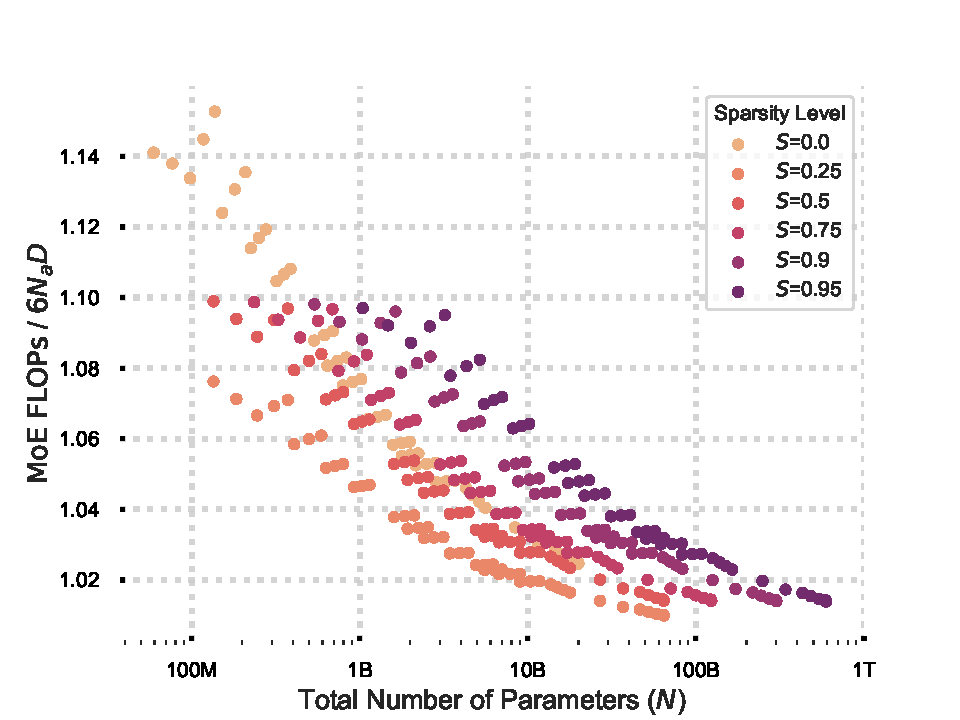
\includegraphics[width=0.8\textwidth]{plots/appendix/app_flop_6nd-v2.pdf}
    \caption{\textbf{Accuracy of $6N_aD$ FLOPs Estimator for MoEs}.
    Ratio of the MoE FLOPs estimator (\Cref{eq:flops}) to the $6N_aD$ estimator as a function of the total number of parameters, for a fixed context length of $D = 2048$, used in our experiments.}
    \label{fig:flop_6nd_v2}
\end{figure}

\begin{comment}
\subsection{Counting Theoretical Flops}
\label{app:count_flops}
Let:
\begin{itemize}
    \item $d_{\text{model}}$ denote the embedding dimension
    \item $G$ denote the granularity (default is 1)
    \item $E_{\text{total}}$ denote the total number of experts
    \item $E_{\text{top-k}}$ denote the number of active experts
    \item $n_{\text{layers}}$ denote the number of layers
    \item $n_{\text{ctx}}$ denote the context length
\end{itemize}

Assume:
\begin{itemize}
    \item All layers are MoE layers
    \item We are using GLU experts instead of MLP experts
    \item The hidden dimension of GLU experts is $d_{\text{ffn}} = 4 \cdot d_{\text{model}}$
\end{itemize}

Forward-and-backward FLOP constants:
\begin{itemize}
    \item For linear projections: $c_L = 6$
    \item For MoE routing: $c_R = 14$ (following ~\citet{ludziejewski2024scaling})
\end{itemize}

FLOPs per token per transformer block:
\begin{itemize}
    \item \textbf{Attention QKV and projection:} $c_L \cdot 2d^2_{\text{model}}$ (with a factor of 2 to account for fewer transformations)
    \item \textbf{Attention logits and values:} $c_L \cdot 2d_{\text{model}} n_{\text{ctx}}$
    \item \textbf{Router:} $c_R \cdot d_{\text{model}} E_{\text{total}}$
    \item \textbf{MoE:} $c_L \cdot 3 d_{\text{ffn}} d_{\text{model}} E_{\text{top-k}} = c_L \cdot \frac{12}{G} d^2_{\text{model}} E_{\text{top-k}}$
    \item \textbf{Final unembedding layer:} $c_L \cdot n_{\text{vocab}} d_{\text{model}}$
\end{itemize}

To simplify, we can skip router FLOPs because $\frac{E_{\text{total}}}{d_{\text{model}}}$ is quite small.
Thus, FLOPs per token simplifies to:
\begin{equation*}
   n_{\text{layers}} \cdot d^2_{\text{model}} \Big( 4c_L + \frac{12c_L}{G} E_{\text{top-k}} + 2c_L \frac{n_{\text{ctx}}}{d_{\text{model}}} + c_L \frac{n_{\text{vocab}}}{d_{\text{model}} n_{\text{layers}}}\Big)
\end{equation*}



% \begin{equation}
%  n_{\text{layers}} \cdot d^2_{\text{model}} \left( 2c_L + \frac{12c_L}{G} E_{\text{top-k}} + 2c_L \frac{n_{\text{ctx}}}{d_{\text{model}}} + c
% \end{equation}




% \Samira{The main problem with this approach is that our cost function is only a function of theoretical flops, whereas in practice costs related to memory and communication can be an important bottleneck, hence the assumption that we infinitely grow total number of parameters and have a fixed training/inference cost for a sparse mixture of expert model as long as number of active parameters is the same is not realistic.}

% \Samira{The fact that the cost function is only a function of theoretical flops is not a big issue for scaling law studies that consider architectures where number of parameters and flops have a linear relation, but in our case this is not the case, as we can increase the total number of parameters almost independently of the number of active parameters which linearly interact with the number of theoretical flops.}

% %Theory
% \paragraph{Theoretical Flops}
% \paragraph{Memory}
% \paragraph{Communication across Experts}

% \begin{equation}
%  \text{Total Cost} = \alpha \times \text{FLOPs} + \beta \times \text{Memory Cost} + \gamma \times \text{Communication Cost}
% \end{equation}
% Adjusting the weights in the equation for total cost involves determining the relative importance of FLOPs, memory cost, and communication cost which depends on hardware and infrastrcure.




% \todo[inline]{In an appendix show what happens if we take memory into account in the cost function (based on some reasonable assumptions that we still need to figure out what they are).}

% Nevertheless, given these results, we  observe that given a limit on the total number of parameters for the model size and the compute budget, there is an optimal sparsity level. In section~\ref{sec:fix_params_vary_sparsity} we further investigate this..
\end{comment}

\clearpage
\section{Additional Analysis}
\subsection{Interplay between parameters and FLOPs per example}
\label{app:n_s_d_interaction}

Recall that in~\Cref{sec:n_s_d_interaction}, we showed that isoFLOP curves were predictive of pretraining loss for different parameter counts and sparsity levels.
In this section, we show similar results with additional training compute budgets.
\begin{enumerate}[left=0pt,itemsep=2pt]
    \item In~\Cref{fig:additional_surfaces}, we first show that IsoFLOP surfaces mapping model size $N$ and sparsity level $S$ to pre-training loss $L$ are predictive in a similar way for all training compute budgets that we consider, ranging from 3e19 to 1e21 FLOPs. 
    \item In~\Cref{fig:additional_surface_eval}, we analyze the fitted IsoFLOP surfaces (one for each training budget) and find that the (a) effect of model size $N$ on optimal \moe sparsity $S^*$ and (b) the effect of \moe sparsity $S$ on the optimal total and active parameters, $N*$ and $N^*_a$, is similar for all training budgets.
\end{enumerate}

\begin{figure}[bp]
    \centering
    \subfigure{%{\textwidth}
        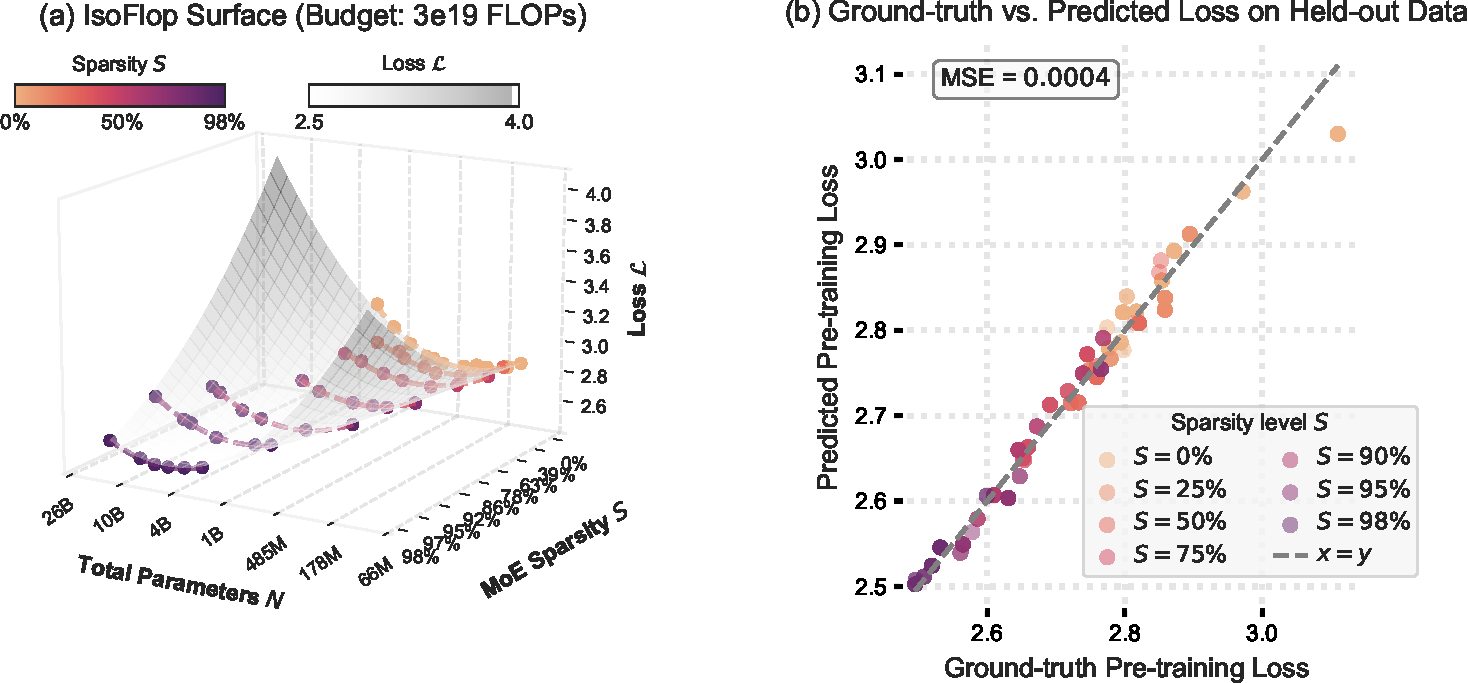
\includegraphics[width=0.45\textwidth]{plots/appendix/app_s2_3e19.pdf}
        \label{fig:isoflop_surface_3e19}
}
\subfigure{%{\textwidth}
        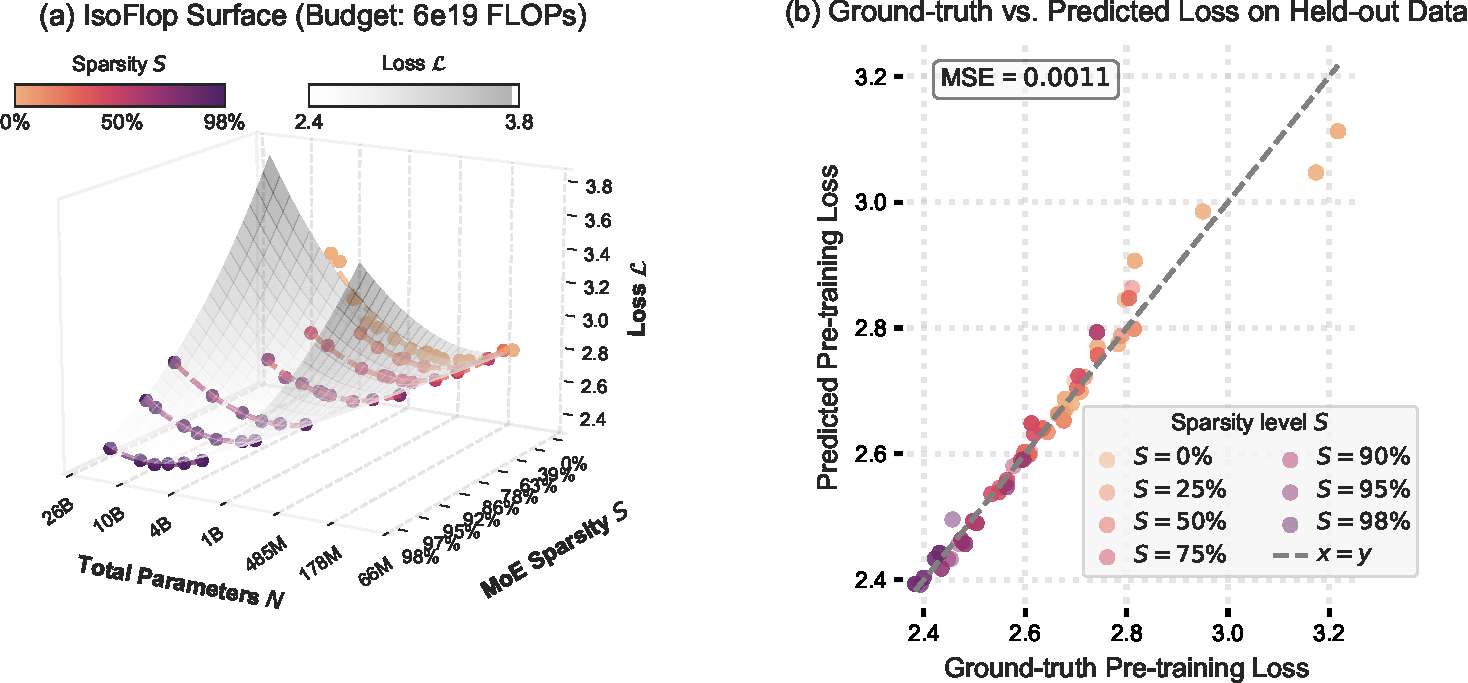
\includegraphics[width=0.45\textwidth]{plots/appendix/app_s2_6e19.pdf}
        \label{fig:isoflop_surface_6e19}
}
\subfigure{%{\textwidth}
        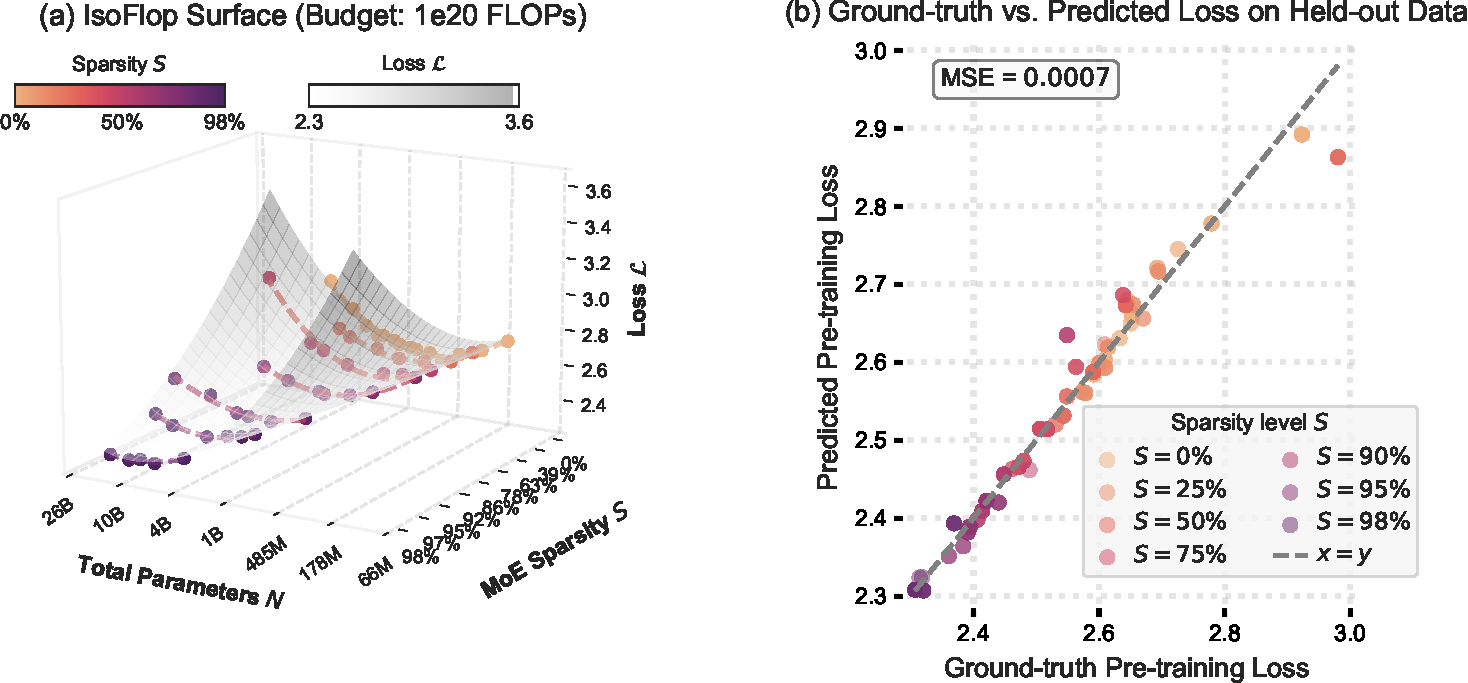
\includegraphics[width=0.45\textwidth]{plots/appendix/app_s2_1e20.pdf}
        \label{fig:isoflop_surface_1e20}
}
\subfigure{%{\textwidth}
        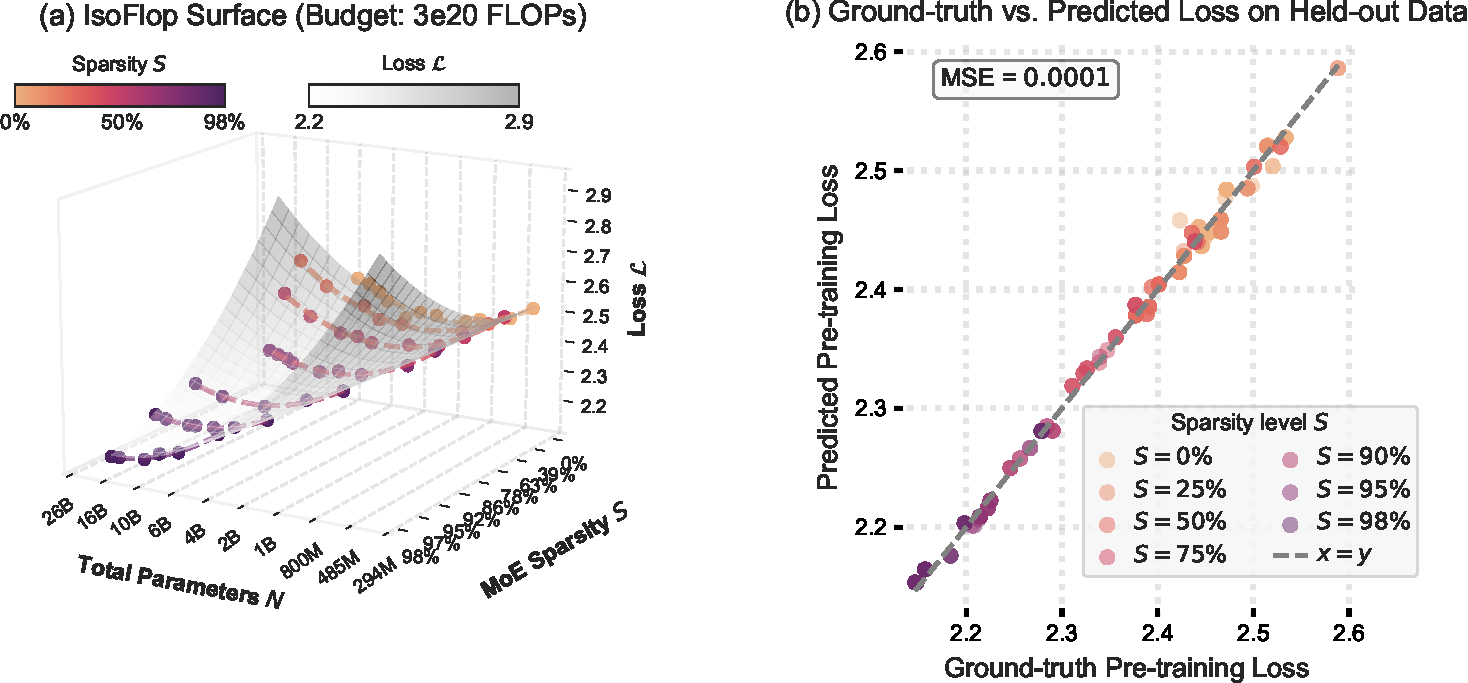
\includegraphics[width=0.45\textwidth]{plots/appendix/app_s2_3e20.pdf}
        \label{fig:isoflop_surface_3e20}
}
\subfigure{%{\textwidth}
        \centering
        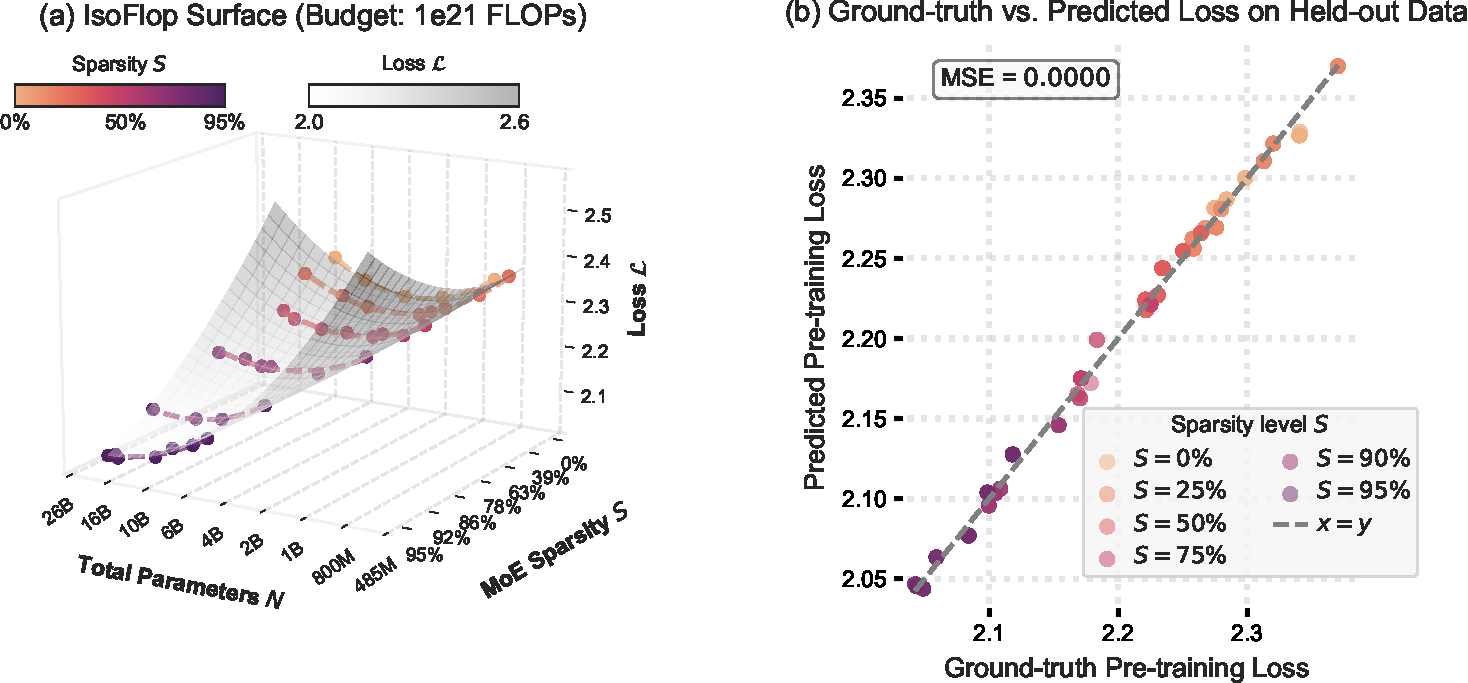
\includegraphics[width=0.45\textwidth]{plots/appendix/app_s2_1e21.pdf}
        \label{fig:s2_sub5}
}
    \caption{
        \textbf{IsoFLOP surfaces over total parameters $N$, \moe sparsity $S$, and pretraining loss $L$ for different compute budgets}. 
        The rows correspond to IsoFLOP surface fitted using models trained with a budget of 3e19, 6e19, 1e20, 3e20, and 1e21.  
        The subplots on the left visualize IsoFLOP surfaces mapping total parameters $N$ and sparsity level $S$ to pretraining loss $L$.
        The subplots on the right correlate the ground-truth pretraining loss with the estimated pretraining loss on held-out data.
        Taken together, these results show that isoFLOP surfaces are accurate proxies for understanding how model size and \moe sparsity jointly impact pretraining loss.
    }
    \label{fig:additional_surfaces}
\end{figure}

\begin{figure}[tbp]
    \centering
    \subfigure{
        \centering
        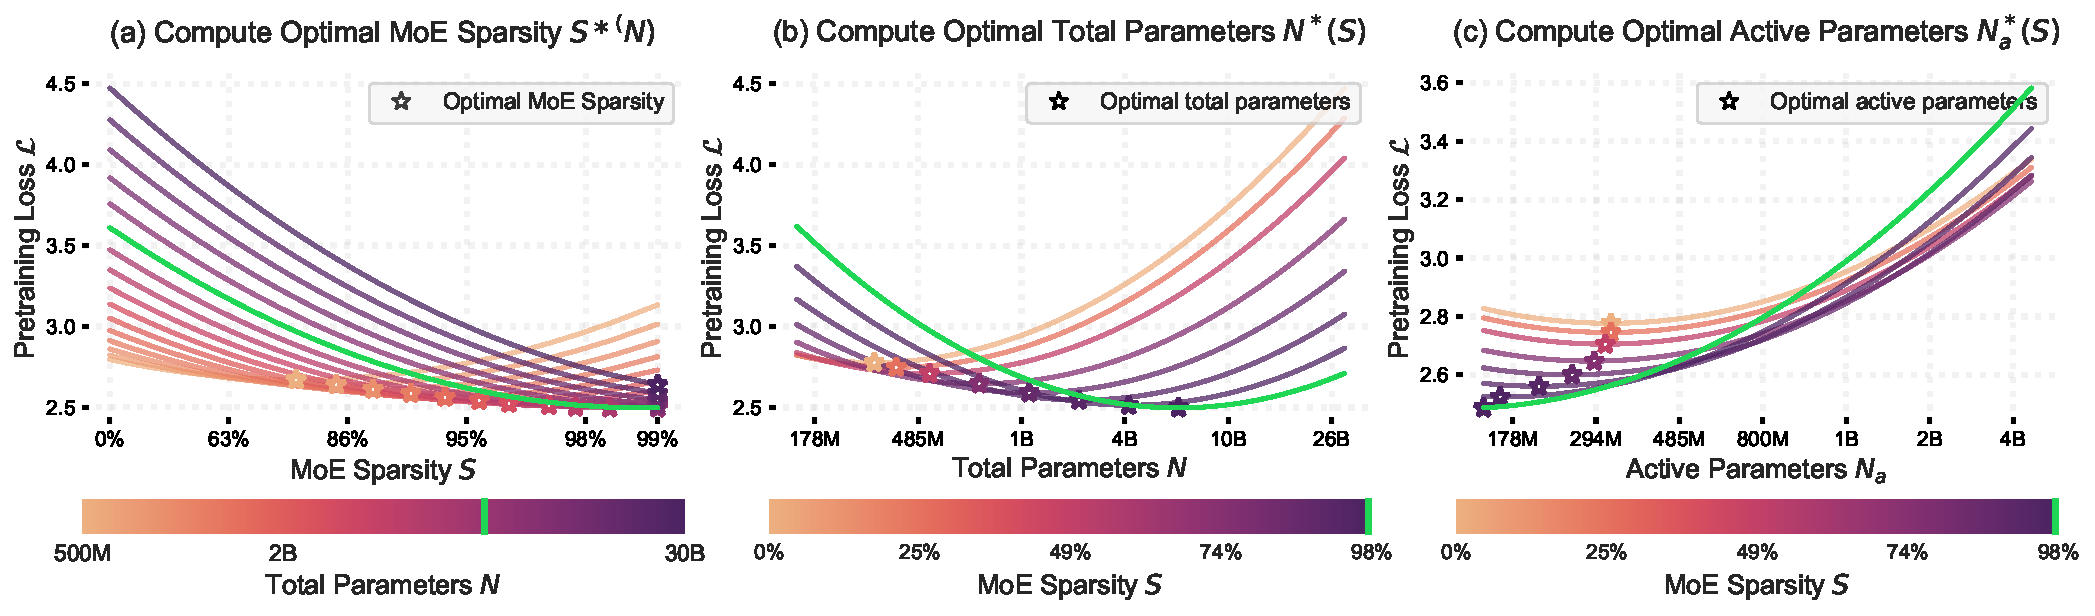
\includegraphics[width=0.45\textwidth]{plots/appendix/app_s2_slices_3e19_fixed_range.pdf}
        \label{fig:slices_3e19}
}    
    \subfigure{
        \centering
        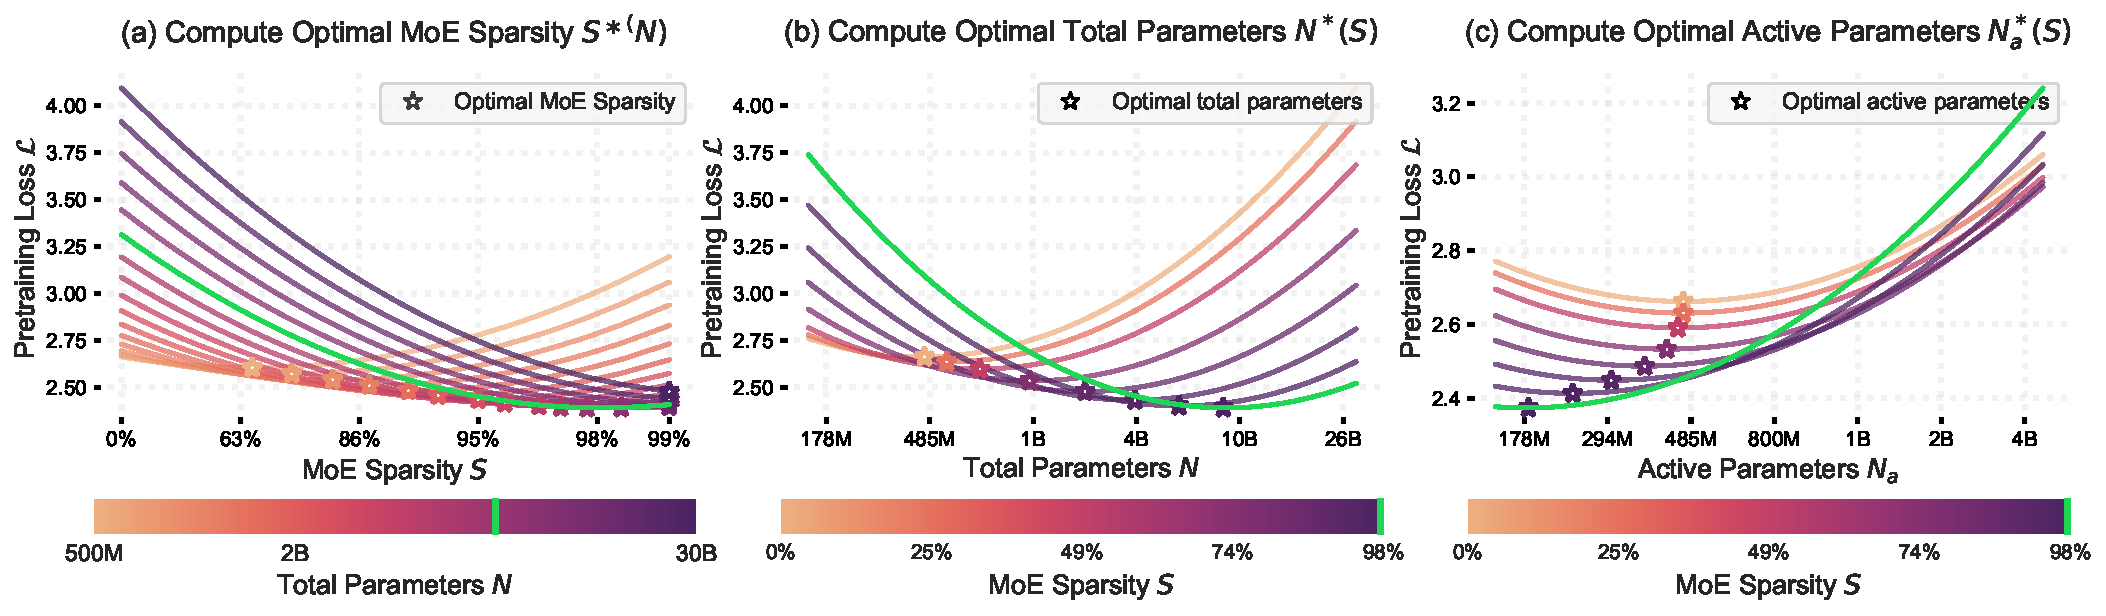
\includegraphics[width=0.45\textwidth]{plots/appendix/app_s2_slices_6e19_fixed_range.pdf}
        \label{fig:slices_6e19}
}
    \subfigure{
        \centering
        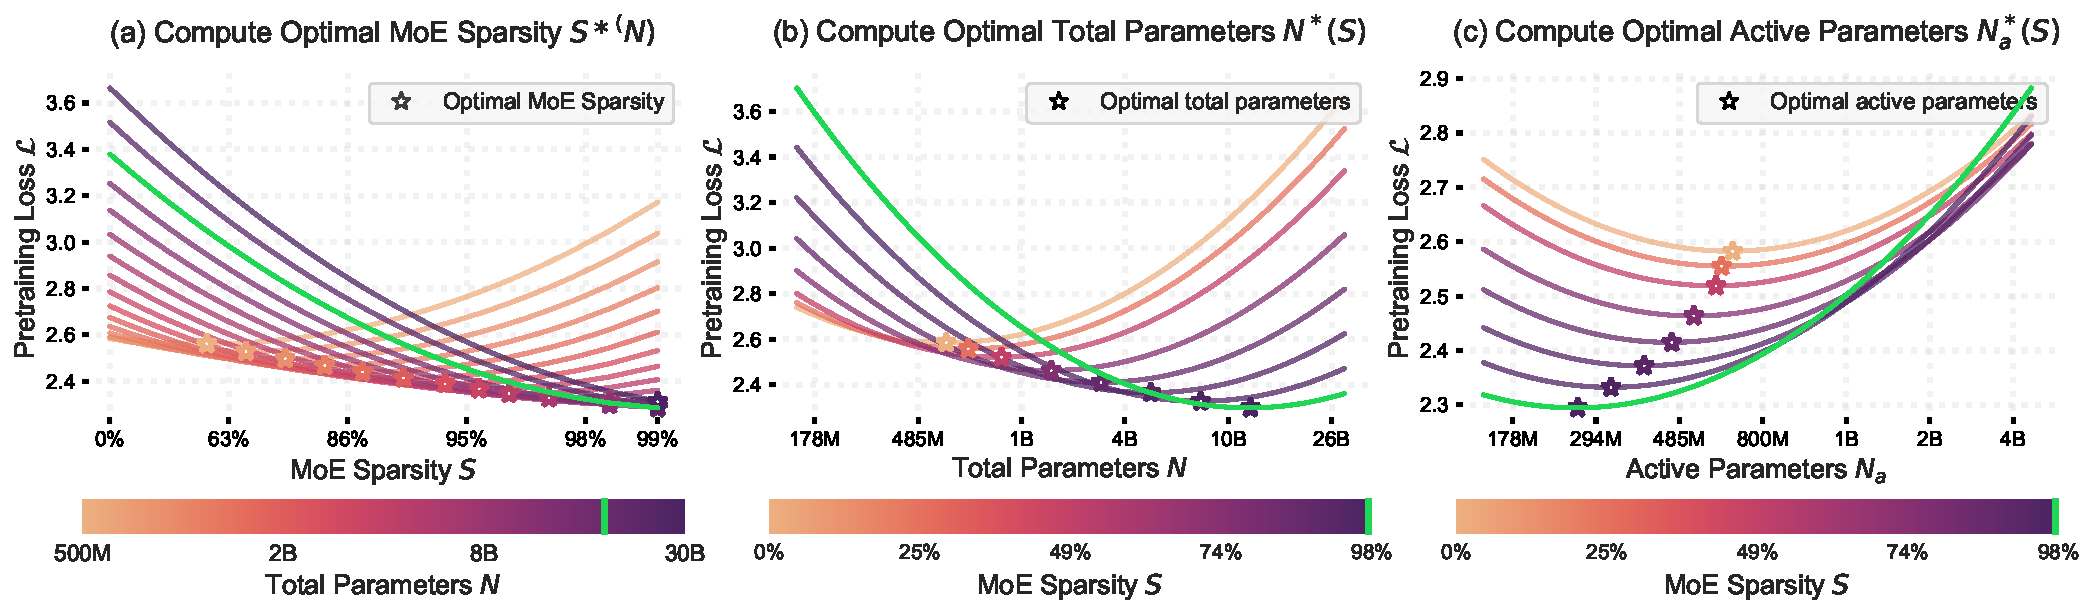
\includegraphics[width=0.45\textwidth]{plots/appendix/app_s2_slices_1e20_fixed_range.pdf}
        \label{fig:slices_1e20}
}
    \subfigure{
        \centering
        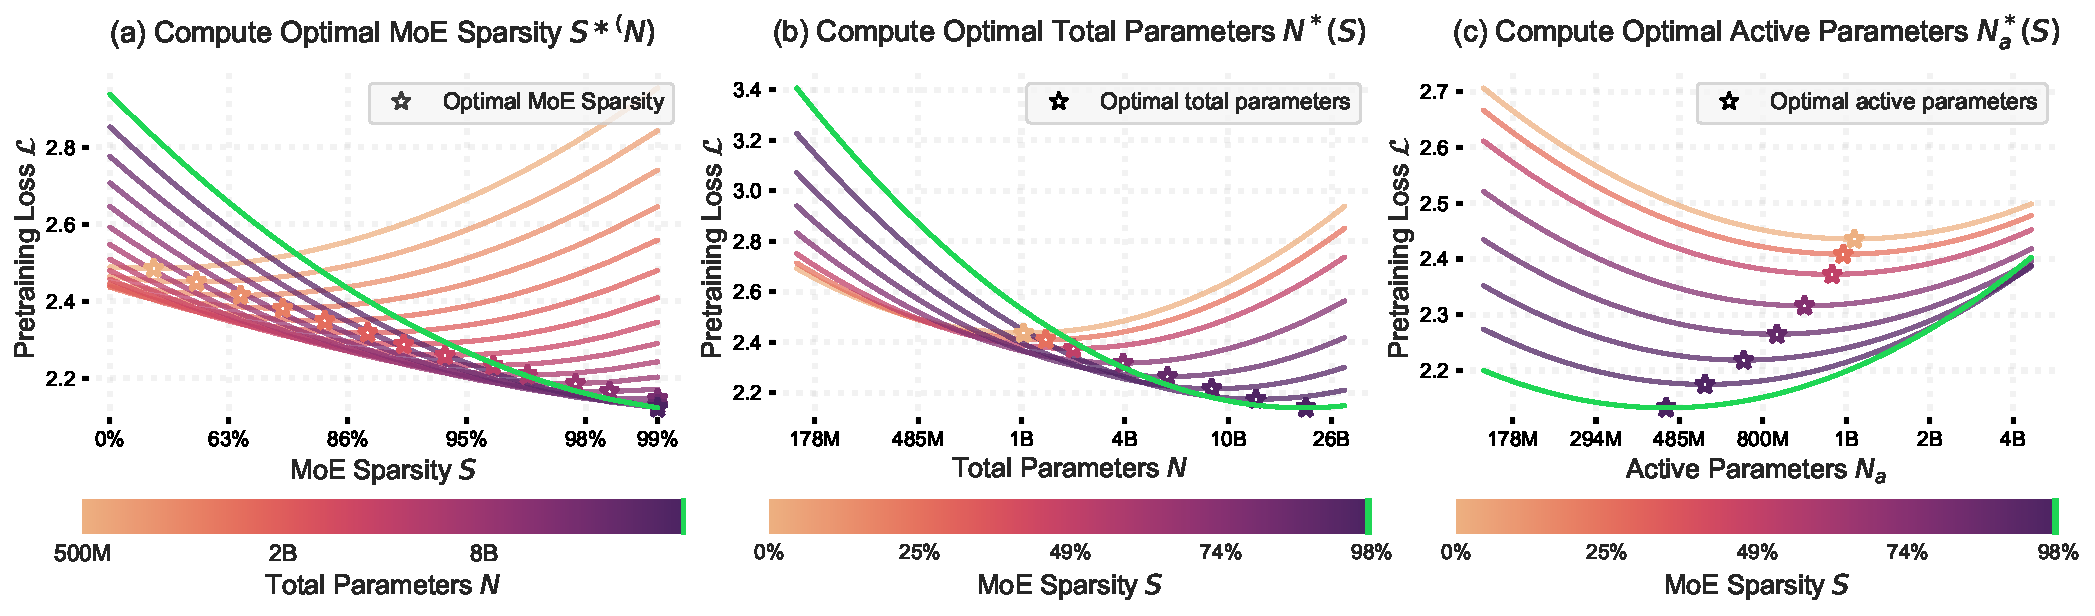
\includegraphics[width=0.45\textwidth]{plots/appendix/app_s2_slices_3e20_fixed_range.pdf}
        \label{fig:slices_3e20}
}    
\subfigure{
        \centering
        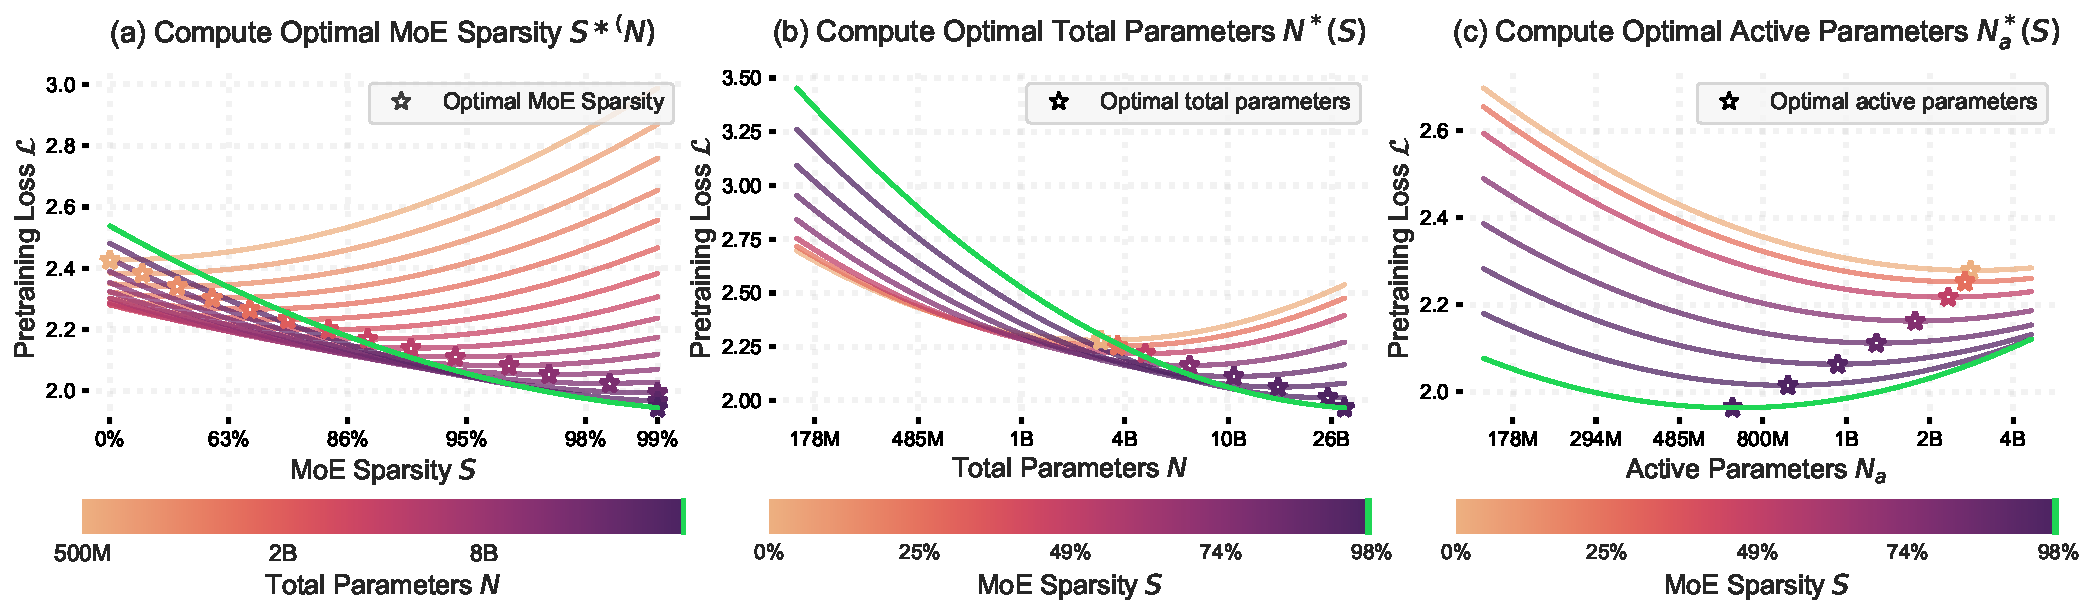
\includegraphics[width=0.45\textwidth]{plots/appendix/app_s2_slices_1e21_fixed_range.pdf}
        \label{fig:slices_1e21}
}
    \caption{
        \textbf{Optimal \moe configurations predictably change with training compute budget.}
        Each row corresponds to an analysis of how optimal \moe sparsity $S^*$, total parameters $N^*$, and active parameters $N^*_a$ change for a given training budget. 
        The subplots on the left show that (a) increasing the training budget increases the model size $N$ (denoted with black dots) with the minimum pretraining loss and (b) for models smaller than a threshold (which increases with training budget), dense models (i.e., $0\%$ sparsity) fare better than sparse \moes. 
        The subplots in the second and third panel show that (a) increasing \moe sparsity increases the optimal total parameters $N^*$ and decreases the optimal active parameters $N^*_a$. In both cases, for a fixed sparsity level, increasing the budget shifts increases the optimal total and active parameters. 
    }
    \label{fig:additional_surface_eval}
\end{figure}


\subsection{Effect of training budget and model size on optimal \moe sparsity}
\label{app:budget}

Recall that in ~\Cref{sec:effect_of_training_budget}, we demonstrated how the relationship between optimal total parameters $N*$, optimal active parameters $N*_a$, and optimal pretraining loss $L$ predictably changes as a function of sparsity $S$ and training budget $C$. 
In this section, we use the fitted isoFLOP surfaces to analyze how the optimal \moe sparsity $S^*$ changes as a function of total parameters $N$ and training budget $C$, as shown in~\Cref{fig:opt_sparsity}. Our main findings are:
\begin{itemize}[left=0pt,itemsep=2pt]
    \item Across all training budgets (ranging from 3e19 to 1e21 FLOPs), increasing the total parameters $N$ leads to an increase in the optimal sparsity level $S^*$. 
    \item For a fixed model size (i.e., total parameters $N$), increasing the training budget $C$ generally reduces the optimal sparsity level $S^*$. 
    \item The relationship between model size $N$ and optimal $S*$ is not linear. For smaller models (up to about $500 \cdot 10^6$  parameters), the optimal sparsity remains at $0$ (i.e., dense) for most compute budgets. 
\end{itemize}



% \newpage
\subsection{Effect of sparsity on downstream task performance}
\label{app:downstream}

In~\Cref{sec:scaling_law_ds}, we analyzed the relationship between upstream pre-training loss and downstream task performance across different \moe sparsity levels. We found that language understanding and world knowledge tasks generally showed a strong correlation between upstream and downstream performance, while reading comprehension tasks seemed to favor denser models to some extent. 

In this section, we provide additional plots for a broader range of tasks within each category to further support our findings. We consider the following tasks:
\begin{itemize}[left=0pt,itemsep=2pt]
\item \textbf{Common Sense Reasoning}: PIQA, CommonSenseQA, OpenBookQA, COPA
\item \textbf{Language Understanding}: LAMBADA, HellaSwag, Winograd, Winogrande
\item \textbf{Reading Comprehension}: SQuAD, CoQA, BoolQ
\item \textbf{World Knowledge}: TruthfulQA, ARC-Easy, ARC-Challenge
\end{itemize}
\Cref{fig:additional_ds_plots} shows the relationship between upstream pre-training loss and downstream task performance for these additional tasks. Each row corresponds to a task category and each subplot represents a different task, with points colored according to \moe sparsity $S$. The $x$-axis represents the upstream pre-training loss, while the $y$-axis shows the downstream task performance metric (usually accuracy or error rate). These results supplement our main findings from \Cref{sec:scaling_law_ds}:
\begin{itemize}[left=0pt,itemsep=2pt]
    \item We observe consistent trends across tasks within each category, with language understanding and world knowledge tasks showing strong correlations between upstream and downstream performance regardless of sparsity. 
    \item Reading comprehension tasks continue to show a slight advantage for denser models, while common sense reasoning tasks (which can be considered part of the symbolic problem-solving category) show more varied relationships between upstream and downstream performance.
\end{itemize}

\begin{figure}[tbp]
    \centering
    \subfigure{
        \centering
        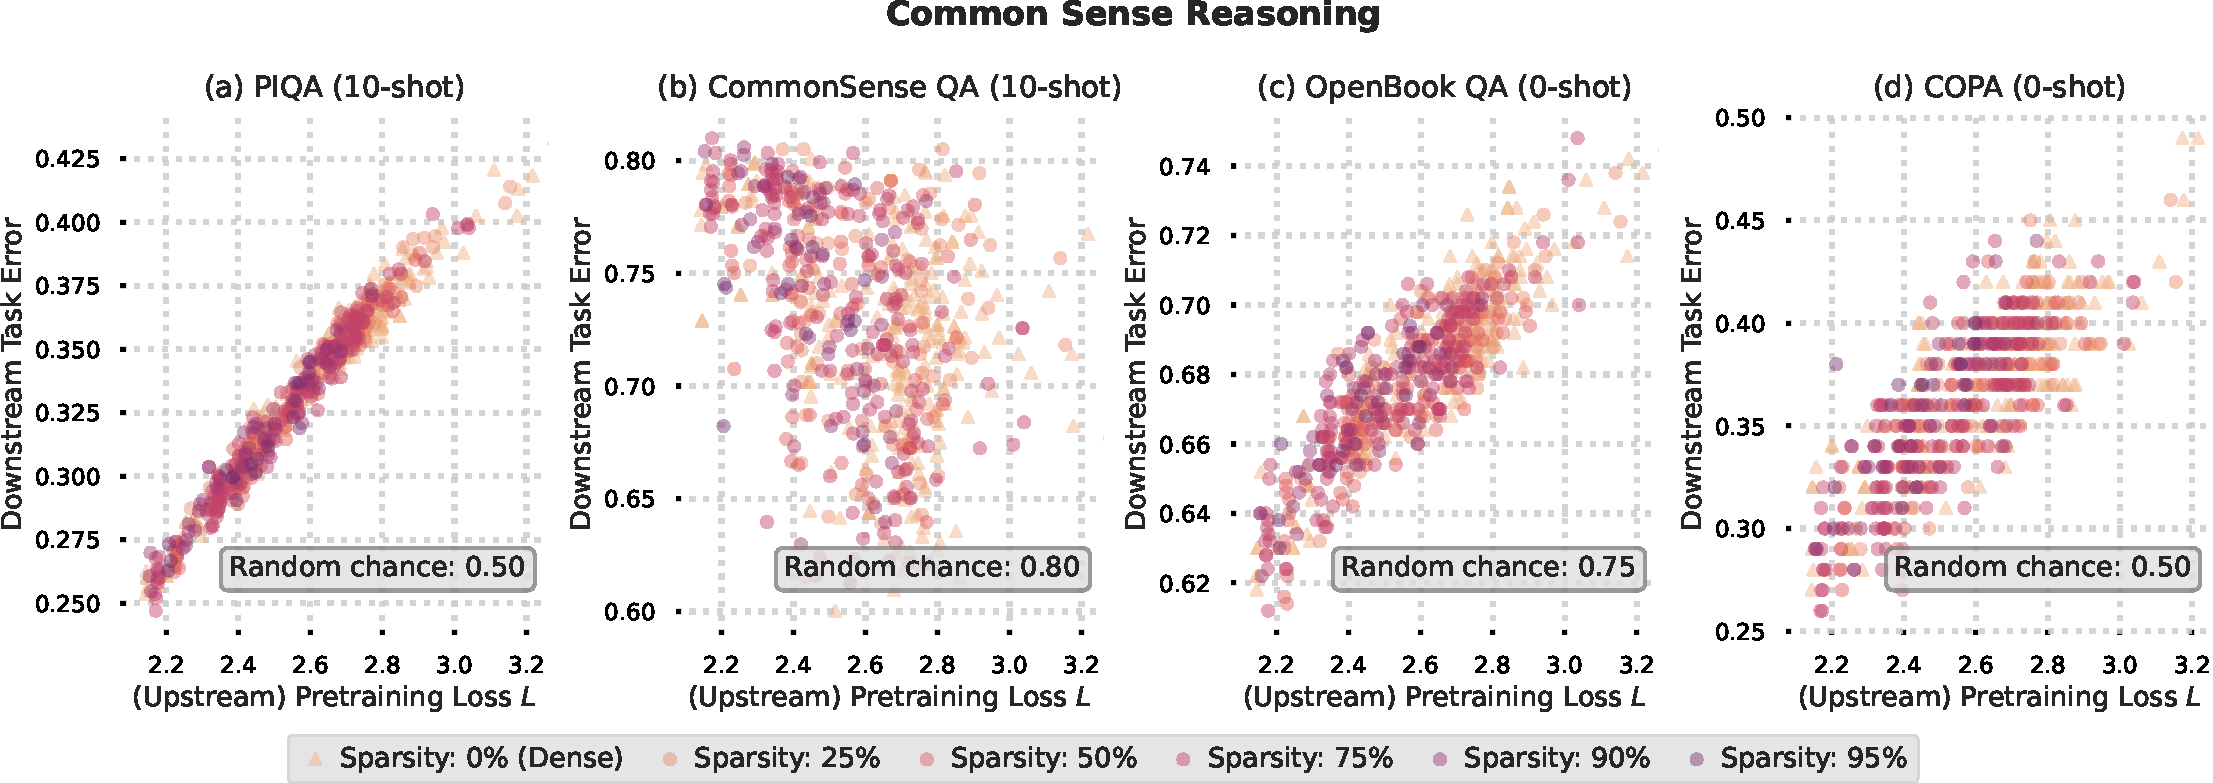
\includegraphics[width=0.75\textwidth]{plots/appendix/app_s4_common.pdf}
        \label{fig:s4_sub1}
}    \subfigure{
        \centering
        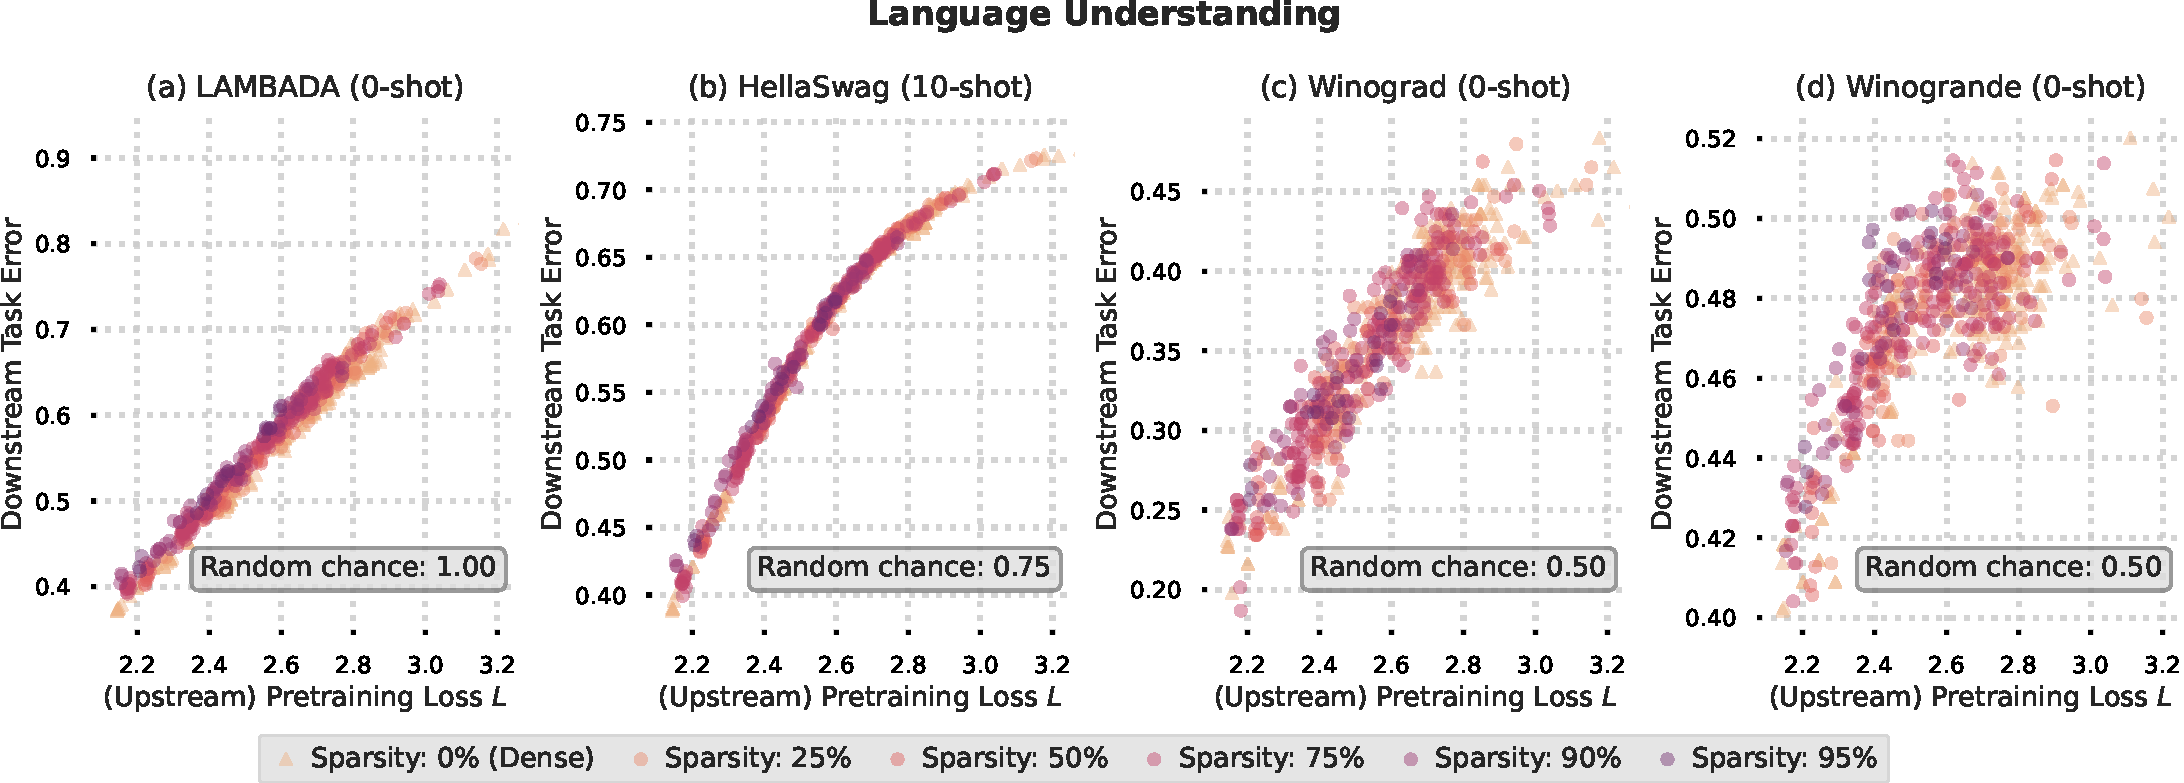
\includegraphics[width=0.75\textwidth]{plots/appendix/app_s4_language.pdf}
        \label{fig:s4_sub2}
}    \subfigure{
        \centering
        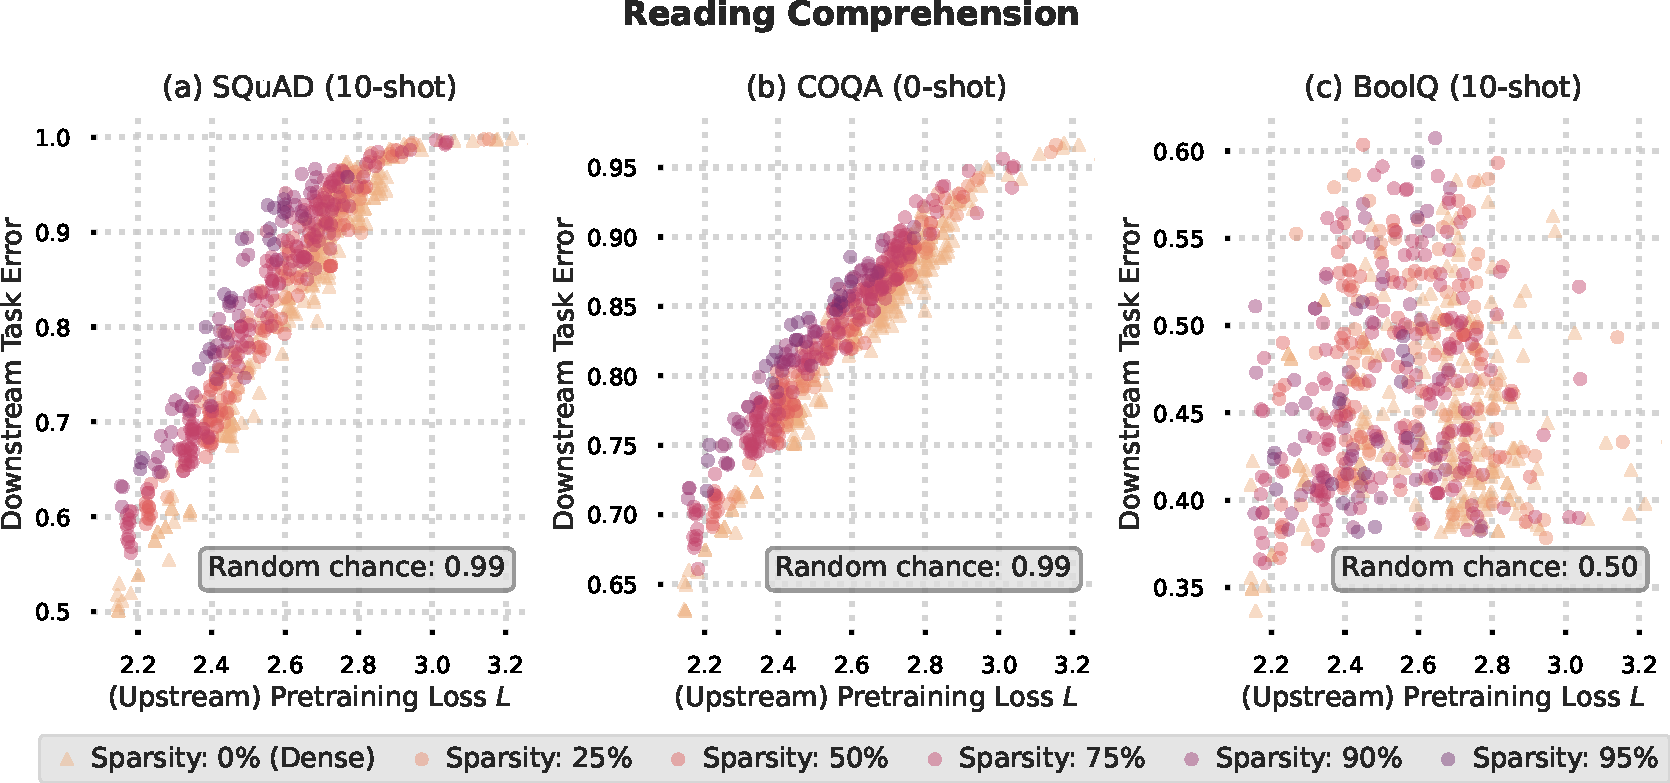
\includegraphics[width=0.6\textwidth]{plots/appendix/app_s4_reading.pdf}
        \label{fig:s4_sub3}
        \par\medskip
}    \subfigure{
        \centering
        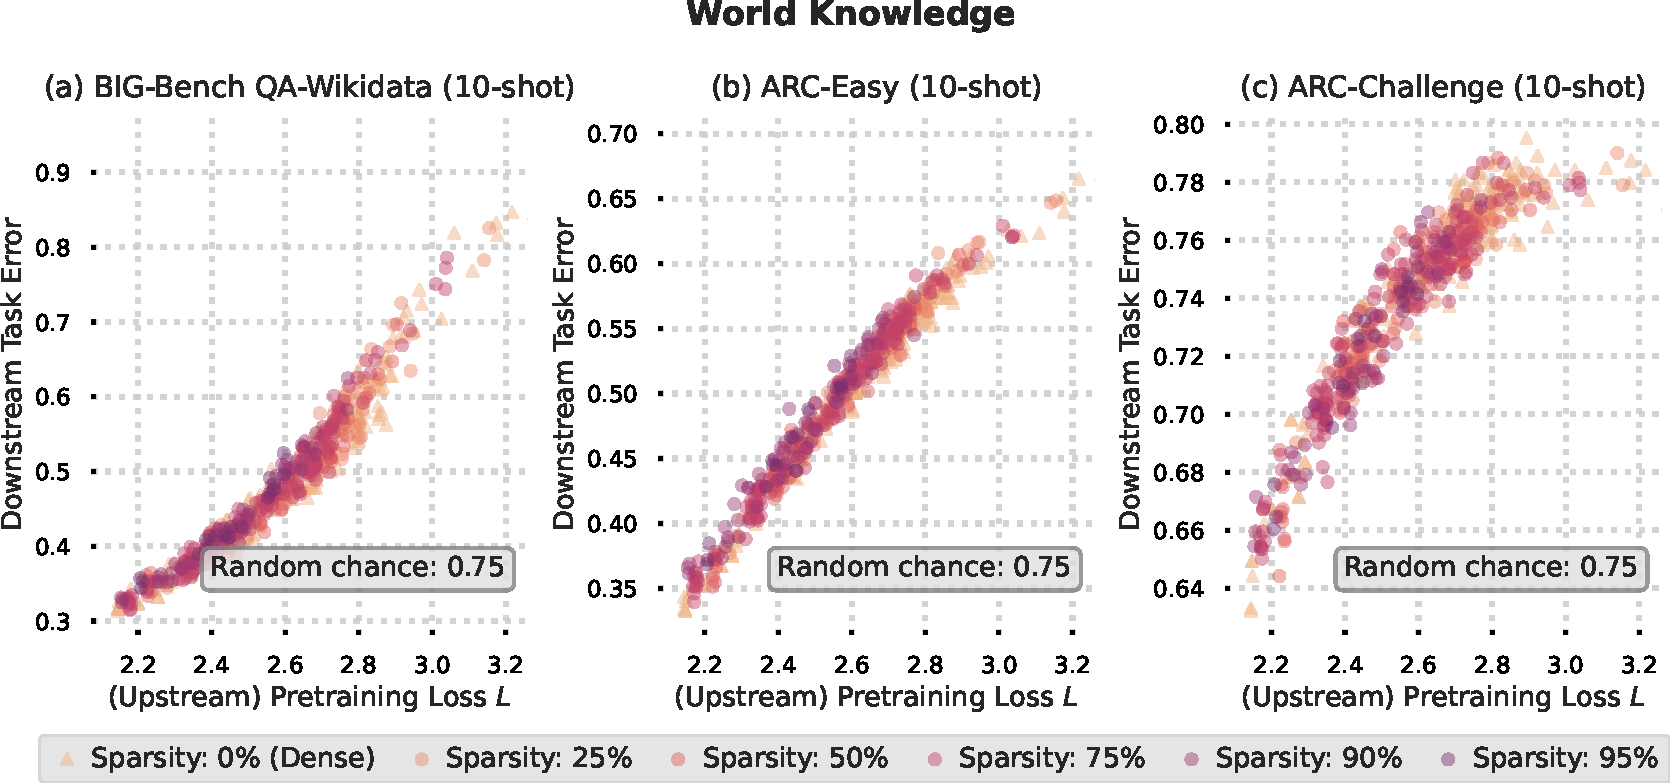
\includegraphics[width=0.6\textwidth]{plots/appendix/app_s4_world.pdf}
        \label{fig:s4_sub4}
}    \caption{
        \textbf{Downstream task performance vs. upstream pre-training loss.} 
        Each subplot shows the relationship between upstream pre-training loss (x-axis) and downstream task performance (y-axis) for a specific task. 
        Similar to our results in~\Cref{sec:scaling_law_ds}, we find that the \moe sparsity level does not change the relationship between upstream pre-training loss and downstream task performance.  
    }
    \label{fig:additional_ds_plots}
\end{figure}

\subsection{Comparing IsoFLOP Surface Analysis with Independent 2d IsoFLOPs}
\label{app:validating_isoflop}

Recall that in~\Cref{sec:n_s_d_interaction},  we used IsoFLOP surfaces that predict pre-training loss across varying parameter counts and sparsity levels to understand how optimal sparsity and optimal model size depend on each other. 

In this section, we evaluate whether these findings remain consistent when we do not rely on fitted IsoFLOP surfaces.
Specifically, similar to Approach II in~\citet{hoffmann2022training}, we directly fit univariate quadratic functions that map model size $N$ to pre-training loss $L$, independently for each sparsity level and training compute budget. We then assess these univariate fits to determine whether our findings in~\Cref{sec:n_s_d_interaction} hold.

% In~\Cref{fig:chinchilla}, each row shows how the optimal total and active parameters change as a function of MoE sparsity for fixed training budgets. As in our findings from~\Cref{sec:n_s_d_interaction}(\Cref{fig:iso_surface_sliced}), increasing sparsity increases the optimal total parameters while decreasing the optimal active parameters. Moreover, larger compute budgets still result in higher optimal total and active parameters, regardless of the sparsity level.

\begin{itemize}[left=0pt,itemsep=2pt]
    \item In~\Cref{fig:chinchilla}, each row shows how the optimal total and active parameters change as a function of MoE sparsity for fixed training budgets. As in our findings from~\Cref{sec:n_s_d_interaction} (\Cref{fig:iso_surface_sliced}), increasing sparsity increases the optimal total parameters while decreasing the optimal active parameters. Moreover, larger compute budgets still result in higher optimal total and active parameters, regardless of the sparsity level.
    \item Furthermore, in~\Cref{fig:effect_of_sparsity_on_loss}, we observe that across all training compute budgets, increasing sparsity reduces the optimal pre-training loss. This is consistent with the trends identified in~\Cref{sec:effect_of_training_budget} (\Cref{fig:effect_of_compute}), thereby validating our earlier results.
\end{itemize}
% \begin{figure}[!h]
%     \centering
%     \includegraphics[width=\textwidth]{plots/approach_2.pdf}
%     \caption{
%     \textbf{Approach 2 main plot.}
%         \Harshay{reminder to update plot if we decide to remove 1e21}
%     Notebook: \url{https://github.pie.apple.com/sabnar/l3m_core/blob/hs/notebooks/approach2_new.ipynb}
%     }
%     \label{fig:approach2}
% \end{figure}
% skip for now this is mre of the same thing as sparsity comparison 
\begin{figure}[tbp]
    \centering
    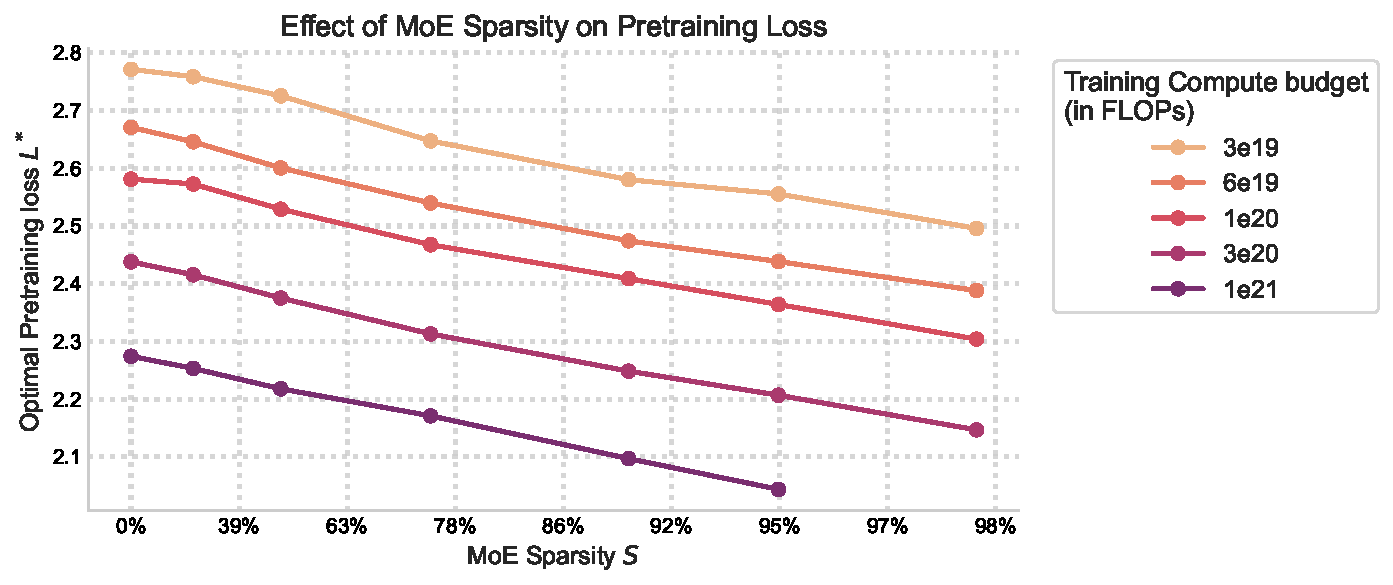
\includegraphics[width=0.7\textwidth]{plots/appendix/effect_of_sparsity_on_loss_thresholded.pdf}
    \caption{
    \textbf{Effect of \moe sparsity on pretraining loss across different training compute budgets}. 
    As sparsity increases, the validation loss decreases for all compute budgets, with larger budgets (darker lines) achieving lower losses at each sparsity level.
    This trend is consistent with the findings from~\Cref{sec:effect_of_training_budget}, demonstrating that increasing sparsity reduces the optimal pretraining loss across all compute budgets.
    % \todo[inline]{change this plot to log scale}
    % \Harshay{reminder to update plot if we decide to remove 1e21}
    % Notebook: \url{https://github.pie.apple.com/sabnar/l3m_core/blob/hs/notebooks/approach_2_sparsity_comparison.ipynb}
    }
    \label{fig:effect_of_sparsity_on_loss}
\end{figure}

\begin{figure}[tbp]
    \centering
    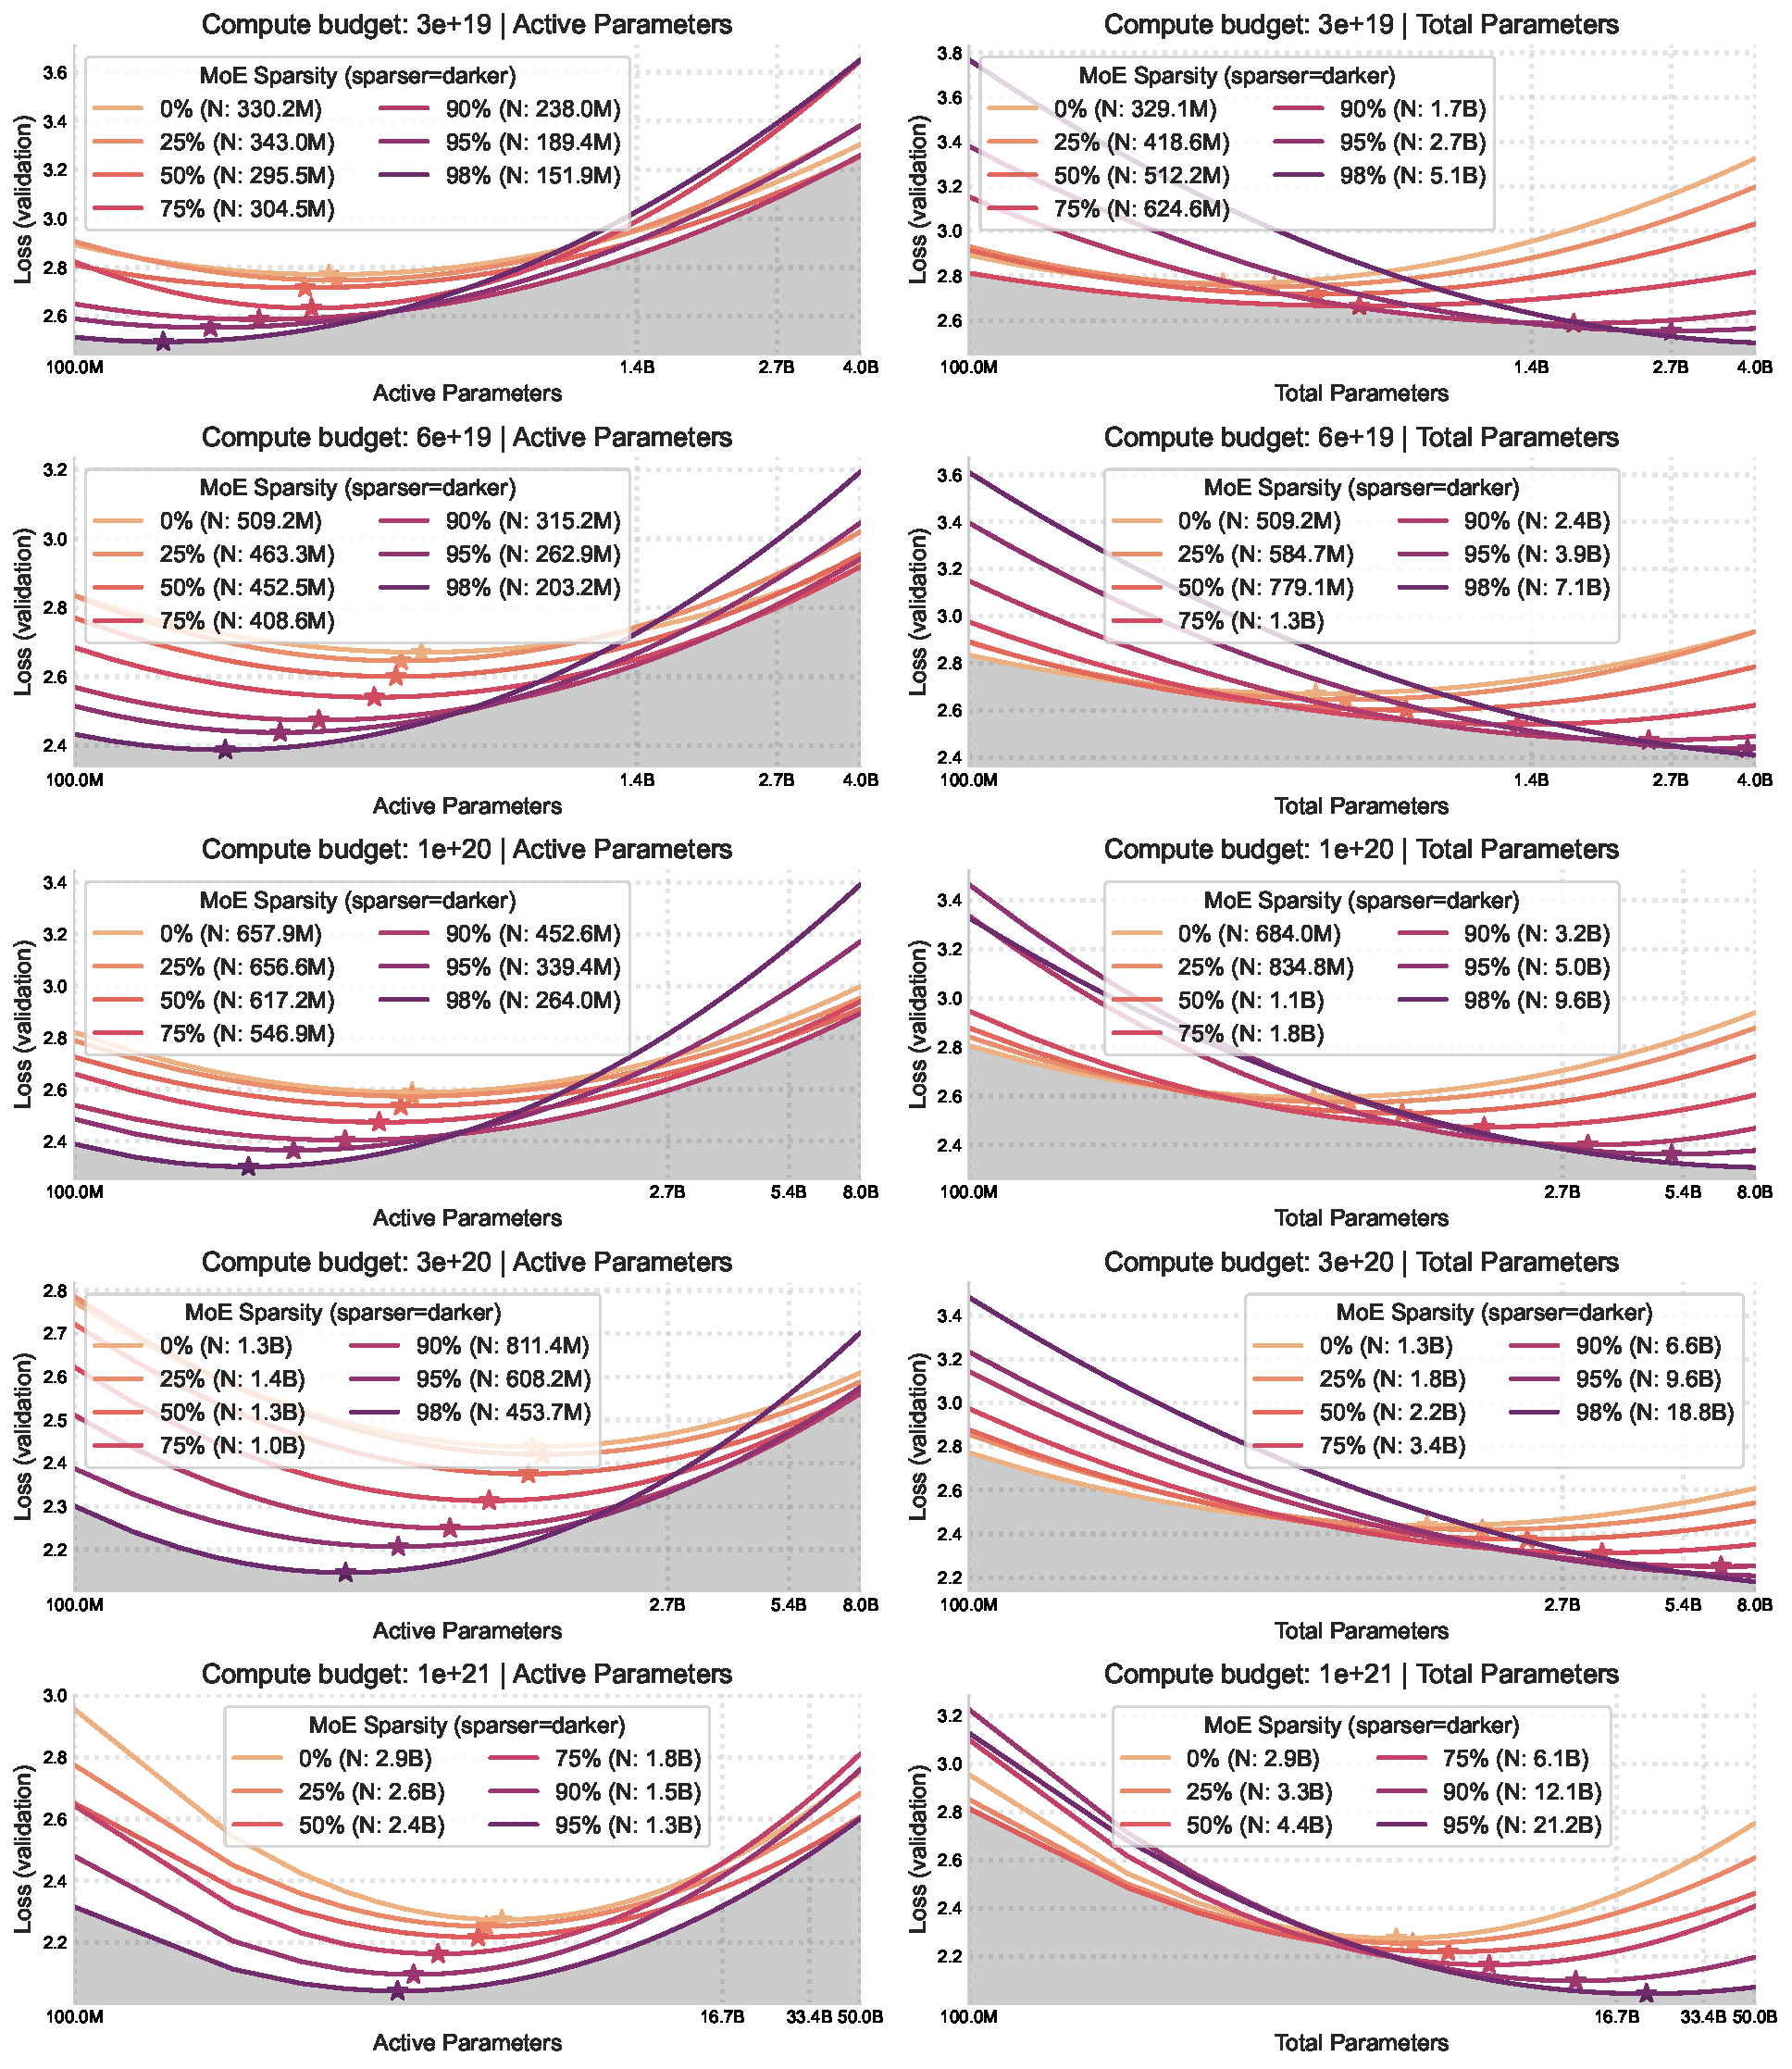
\includegraphics[width=0.8\textwidth]{plots/appendix/approach_2_sparsity_comparison_thresholded.pdf}
    \caption{
    \textbf{Effect of \moe sparsity on optimal total and active parameters across different training compute budgets.} 
    Each row shows the change in total and active parameters as a function of sparsity level for fixed training budgets. 
    Increasing sparsity leads to an increase in the optimal total parameters while reducing the optimal active parameters, consistent with our findings in~\Cref{sec:n_s_d_interaction} (\Cref{fig:iso_surface_sliced}). 
    Larger training compute budgets result in higher optimal (total and active) parameters across all sparsity levels.
    % \Harshay{reminder to update plot if we decide to remove 1e21}
    }
    \label{fig:chinchilla}
\end{figure}


% \input{appendices/effect_of_sparsity_on_scaling_laws}
\section{Does Chain-of-Thought prompting benefit sparse MoEs more than dense models?}
\label{app:cot_expt}

In~\Cref{sec:scaling_law_ds}, we observed that dense models fare marginally better than sparse MoEs on reading comprehension tasks, potentially due to the higher inference-time compute of a dense model than a perplexity-matched sparse MoE. 
Then, in~\Cref{sec:discussion}, we hypothesized that alternative strategies to increase inference-time compute may reduce the gap between sparse MoEs and dense models on such tasks.
In this section, we test this hypothesis by leveraging a ``length-controlled'' variant of few-shot Chain-of-Thought (CoT) prompting to indirectly control inference-time compute. We then use this to study the effect of inference-time compute on downstream task performance of dense and MoE models.  

\paragraph{Experiment setup.}
We evaluate Qwen1.5 models~\citep{qwen} on the GSM8k dataset~\citep{cobbe2021gsm8k} to study the effect of few-shot CoT prompting~\citep{wei2022chain_cot} on downstream task performance. 
We look at the effect of increasing inference-time compute (via CoT prompting) on GSM8k performance of dense models with sizes ranging from 0.5B to 14B and a 5x2.7B sparse MoE. 
We also use $10$ fixed examples from the GSM8k train split as few-shot examples for all runs.

\paragraph{Length-controlled CoT prompting enables control over inference-time compute.}
Given an instruction-tuned model and a problem from the GSM8k dataset, we control the inference-time compute of the model by controlling the number of tokens generated to output the final answer to the given problem. 
To do so, we observe that providing instructions via system prompts (with few-shot CoT prompting) does not effectively control the number of generated tokens and, as a result, inference-time compute. 
We also observe that the average number of tokens in the few-shot GSM8k answers (provided in-context) strongly influences the number of tokens generated by the model to solve the given GSM8k question. 
Therefore, similar to work on designing GSM8k variants to analyze language modeling phenomena~\citep{mirzadeh2024gsm,li2024gsmplus,zhang2024careful}, we prompt an instruction-tuned model---{Llama-3.1-70b}~\citep{dubey2024llama} in our experiment---to rewrite GSM8k answers in approximately $k \in \{5,\dots,100\}$ words.
Then, we use the paraphrased GSM8k examples as few-shot examples to indirectly control the number of generated tokens. 
As shown in \Cref{fig:cot_effect}(a), this approach enables systematic control over the length of paraphrased answers.
The strong correlation ($\rho=0.88$) between few-shot and generated answer lengths in \Cref{fig:cot_effect}(b) validates that our approach effectively modulates inference-time compute.

\begin{figure}[H]
    \centering 
    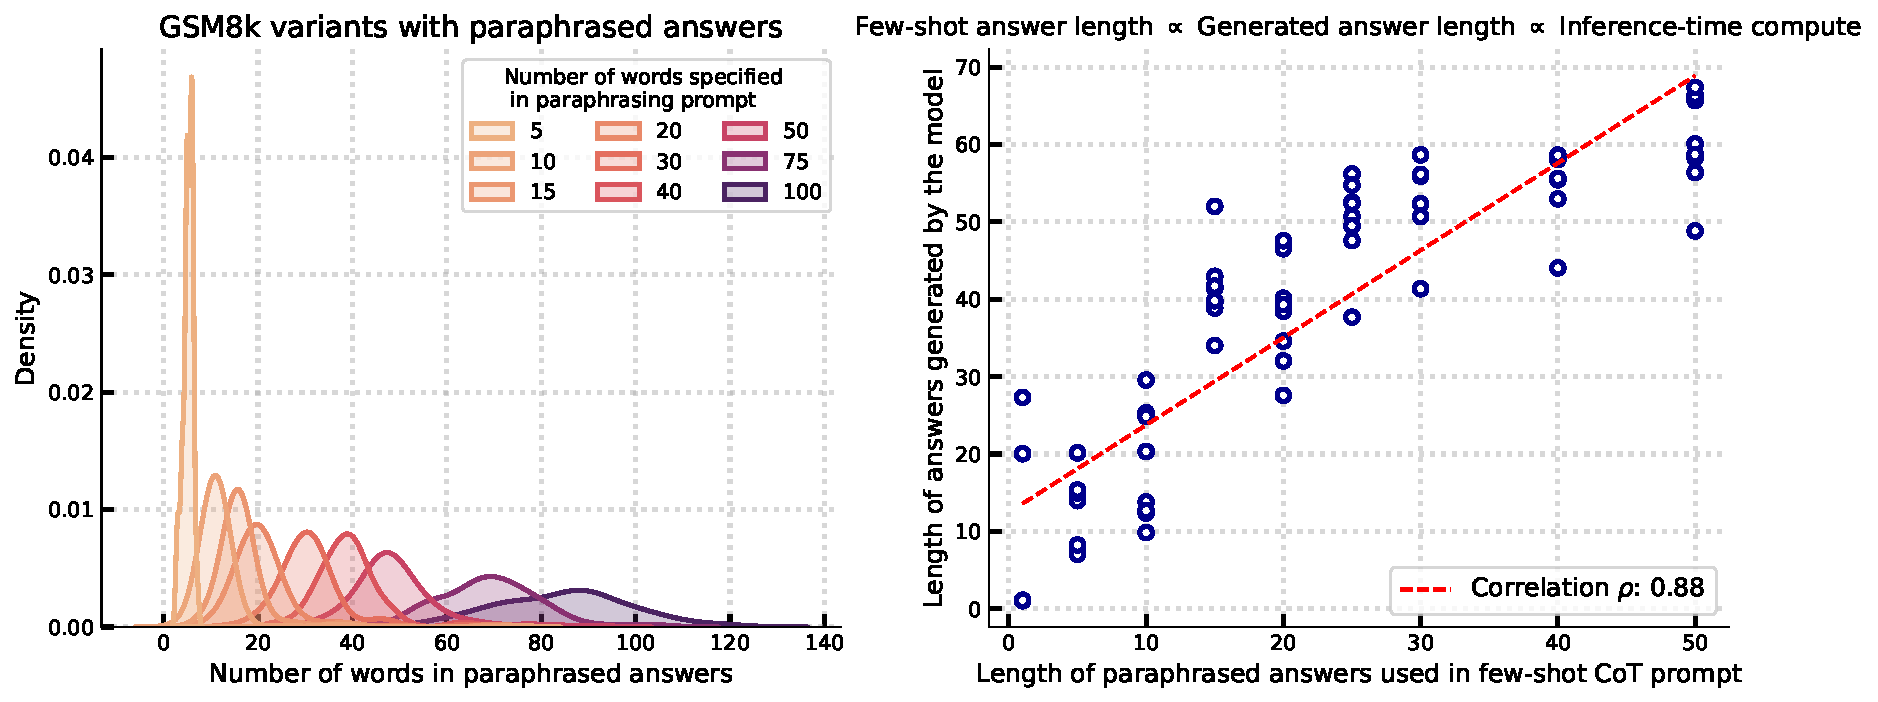
\includegraphics[width=0.8\textwidth]{plots/effect_of_cot.pdf}
    \caption{
        \textbf{Varying inference-time compute via length-controlled Chain-of-Thought prompting.}
        We can control inference-time compute (number of generated tokens) via Chain-of-Thought prompting in two steps: (a) generating paraphrased GSM8k answers of varying lengths (5-100 words) and (b) using paraphrased answers as few-shot examples in CoT prompts to influence the length of generated answers determine the model's output length ($\rho=0.88$ correlation). The systematic shift in answer length distributions in subplot (a) and the linear relationship between few-shot answer length and generated answer lenth ($\rho=0.88$ correlation) in (b) validate that our prompting approach effectively modulates inference-time compute, enabling controlled studies of its impact on model performance.
    }
    \label{fig:cot_effect}
\end{figure}

\paragraph{Effect of length-controlled CoT on downstream task performance.}
We investigate how inference-time compute affects GSM8k performance across Qwen1.5 models using $10$-shot length-controlled CoT prompting, varying target answer lengths $k$ from $1$ to roughly $70$ words on average. As shown in~\Cref{fig:cot_effect_perf}, when we increase inference-time compute indirectly through longer generated answers ($x$-axis), we observe a roughly linear improvement in GSM8k performance ($y$-axis) across all model sizes. The linear fits for each model also indicate a pattern through their slopes $m$: larger dense models benefit more from additional inference-time compute. This effect is particularly striking when comparing models at the extremes (i.e., Qwen1.5-0.5B versus Qwen1.5-14B).
% while increasing inference-time compute only improves Qwen1.5-0.5B's performance from $1\%$ to $5\%$, it boosts Qwen1.5-14B's accuracy from $20\%$ to $70\%$.

To analyze whether inference-time compute affects dense and sparse MoE models differently, we examine how the ``performance'' slope $m$ (i.e., accuracy gain per generated word) varies with model size. While the Qwen1.5-5x2.7B MoE cannot be directly compared to dense models due to different active parameter counts, we can account for this by plotting $m$ against the number of active parameters for both architectures. As shown in~\Cref{fig:cot_effect_slope}, when controlling for active parameter count, the MoE model exhibits a higher slope than would be expected from interpolating between dense models. This suggests that MoE models benefit more from dynamically increased inference-time compute compared to dense models with equivalent active parameters.

\begin{figure}[H]
    \centering 
    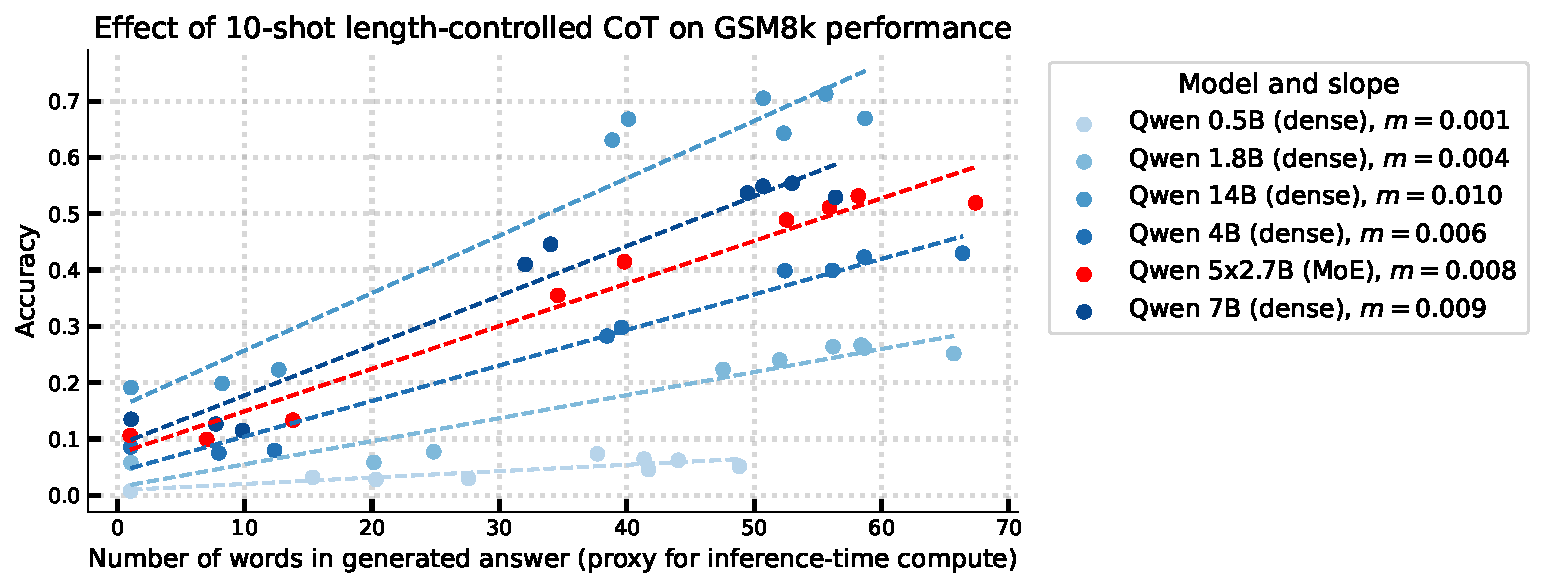
\includegraphics[width=0.92\textwidth]{plots/cot_perf.pdf}
    \caption{
        \textbf{Effect of length-controlled CoT prompting on GSM8k performance across model scales.}
        We evaluate the relationship between inference-time compute (controlled via answer length) and GSM8k accuracy for dense Qwen1.5 models (0.5B-14B parameters) and a 5x2.7B sparse MoE. For all models, increased inference-time compute improves accuracy roughly linearly, with slopes $m$ indicating the marginal effect. Larger dense models show steeper slopes, demonstrating they benefit more from additional inference-time compute—for example, the 14B model's performance improves from 20\% to 70\% as answer length increases, while the 0.5B model improves only from 1\% to 5\%. 
    }
    \label{fig:cot_effect_perf}
\end{figure}

\begin{figure}[H]
    \centering 
    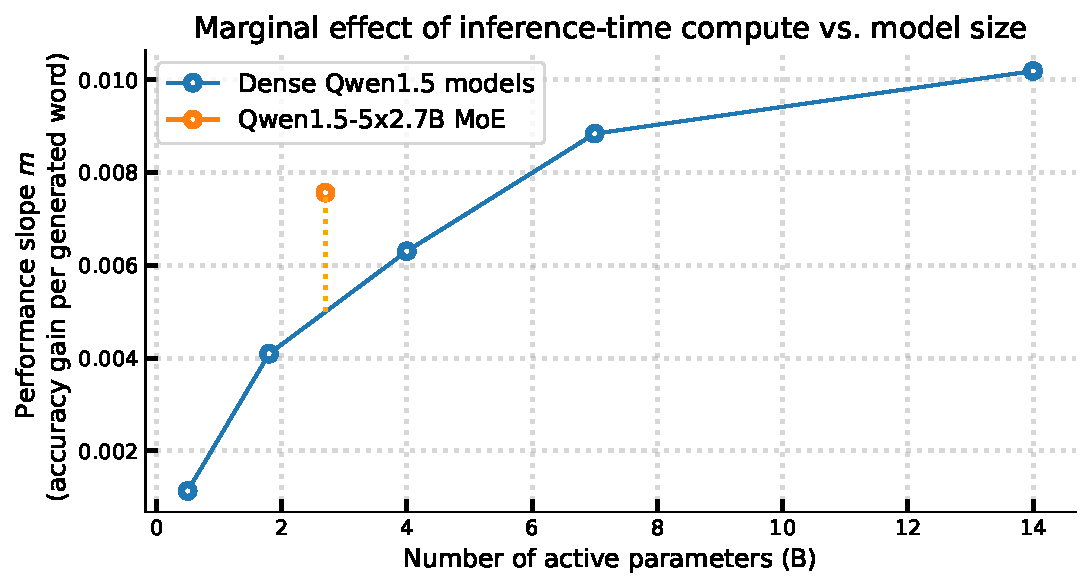
\includegraphics[width=0.55\textwidth]{plots/cot_slope.pdf}
    \caption{
        \textbf{Sparse MoEs benefit more from increased inference-time compute than dense models.}
        We plot the marginal effect of inference-time compute (accuracy gain per generated word) against model size for dense Qwen1.5 models and a 5x2.7B sparse Qwen1.5 MoE. When controlling for the number of active parameters, the MoE model (orange) shows a higher performance slope than would be expected from interpolating between dense models (blue), suggesting that sparse MoEs benefit more from dynamically increased inference-time compute via strategies like CoT prompting.
    }
    \label{fig:cot_effect_slope}
\end{figure}
\newpage
\section{Incorporating Sparsity into Scaling Laws}
\label{appendix:scaling_law_sparsity}

\Cref{tab:lbfgs:hparams} shows the parameters used to initialize L-BFGS used to fit the proposed parametric scaling law given in~\Cref{eq:loss:moe:proposal1}. \Cref{tab:lbfgs:estimate_params} shows the estimated parameters for the parameteric model. We use a held out dataset that consists of data points for models with sparsity value $S = 0.98$ to validate the performance of the estimated model coefficients. The mean squared error and the Huber loss error on the dataset used to fit the model is $0.00056$ and $ 0.0036$ respectively and $0.0058$ and $0.0011$ respectively on the out-of-sample validation set. The quality of the fit measured via the $R^{2}$ metric is $99\%$ on fitting data and $68\%$ on the held out validation dataset.

% \begin{table*}[h]
%     % VT notebook to equation mapping
%     % a, \alpha is C, \lambda
%     \centering
%     \caption{Initial values used to estimate coefficients in \Cref{eq:loss:moe:proposal1}.}
%     \begin{tabular}{c c c c}
%     \toprule
%     $\log(a)$, $\log(b)$, $\log(c)$, $\log(d)$ & $\alpha$, $\beta$, $\gamma$ & $\lambda$, $\delta$ & $\log(e)$ \\
%     \midrule
%     $\left[0, 10, 20 \right]$ & $\left[ 0, 0.25, 0.5, 0.75, 1, 1.25\right]$ & $\left[ -1, -0.5, 0, 0.5, 1\right]$ & $1.5$ \\
%     \bottomrule
%     \end{tabular}
% \label{tab:lbfgs:hparams}
% \end{table*}

% \begin{figure}[ht]
%     \centering
%     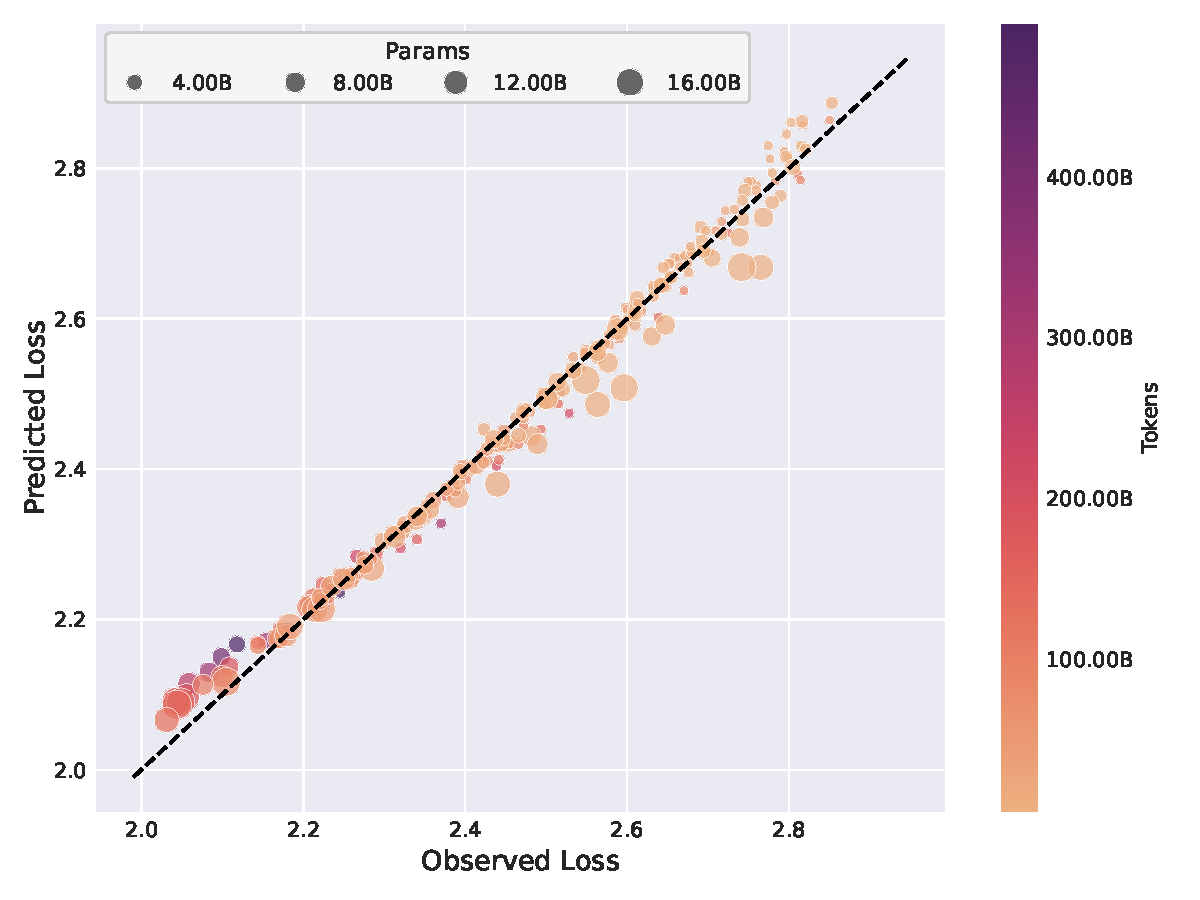
\includegraphics[width=0.48\textwidth]{plots/parameteric_law_interpolation.pdf}
%     \caption{Scaling law fit on data used to estimate coefficients for~\Cref{eq:loss:moe:proposal1}. All $S = 0.98$ data points are excluded from the fitting process to provide an out-of-sample validation show in~\Cref{fig:scaling_law:sparsity98}}.
%     \label{fig:scaling_law:in_sample}
% \end{figure}

\begin{table*}[h]
    % VT notebook to equation mapping
    % a, \alpha is C, \lambda
    \centering
    \caption{Initial values used to estimate coefficients in \Cref{eq:loss:moe:proposal1}.}
    \begin{tabular}{c | c}
    \toprule
    Coefficients & Initial Values \\
    \midrule
    $\log(a)$, $\log(b)$, $\log(c)$, $\log(d)$ & $\left[0, 10, 20 \right]$ \\
    $\alpha$, $\beta$, $\gamma$ & $\left[ 0, 0.25, 0.5, 0.75, 1, 1.25\right]$ \\ 
    $\lambda$, $\delta$ & $\left[ -1, -0.5, 0, 0.5, 1\right]$\\
    $\log(e)$ & $1.5$  \\
    \bottomrule
    \end{tabular}
\label{tab:lbfgs:hparams}
\end{table*}

\begin{table*}[h]
    % VT notebook to equation mapping
    % a, \alpha is C, \lambda
    \centering
    \caption{Estimated values for coefficients in \Cref{eq:loss:moe:proposal1}.}
    \begin{tabular}{c | c}
    \toprule
    Coefficient & Estimate \\
    \midrule
    $\alpha$ & 0.5962 \\
    $\beta$ & 0.3954 \\
    $\lambda$ & -0.1666 \\
    $\delta$ & 0.1603\\
    $\gamma$ & 0.1595 \\
    a & 16612.50 \\
    b & 5455.67 \\
    c & 0.4598 \\
    d & 17.26 \\
    e & 0.94 \\    
    \bottomrule
    \end{tabular}
\label{tab:lbfgs:estimate_params}
\end{table*}

% \clearpage
% \input{appendices/tmp_plots}



\end{document}